% =====================================================================
%  随机信号分析（第5版）  第 3 章  平稳性与功率谱密度
%  由图片型 PDF 扫描件转录重排为 LaTeX 源码
%
%  编译：xelatex   （必须用 XeLaTeX/LuaLaTeX；pdflatex 无法处理中文）
%        xelatex -interaction=nonstopmode -output-directory=<build> <主文件>   （跑四遍）
%
%  本文件是**导言区的唯一权威源**。主文件是 assemble_all 生成物，不要手改。
%  改导言区 → 改这里 → 重跑 `retypeset.py assemble`（或 build/check）。
%
%  ★ 主文件在 \chapter 之前必须有 \setcounter{chapter}{2}
%    否则公式会编成 (1.x)、图会编成 图1.x（原书应为 3.x）。
%    分片单独试编译（harness）时同样要设这个计数器，retypeset.py harness 已代劳。
%
%  ★★ 这个导言区里的每一行几乎都是"踩过坑"换来的，改动前先读
%     .dsh/skills/ssa-textbook/references/pitfalls.md
% =====================================================================
\documentclass[11pt,openany,UTF8]{ctexbook}

% ---------- 页面：还原原书 168mm x 255mm 开本 ----------
\usepackage[%
  paperwidth=168mm,paperheight=255mm,
  top=20mm,bottom=18mm,inner=20mm,outer=16mm,
  headsep=5mm,footskip=8mm]{geometry}

% ---------- 数学 ----------
\usepackage{amsmath,amssymb,amsfonts,mathrsfs}
\usepackage{bm}

% ---------- 图表 ----------
\usepackage{graphicx}          % \resizebox / \scalebox\nobreak：过宽公式压到版心（有先例\nobreak，见 pitfalls\nobreak）
\usepackage{tikz}
\usetikzlibrary{patterns,arrows.meta,positioning,calc}
\usepackage{wrapfig}
\usepackage{booktabs}
\usepackage{array}
\usepackage{multirow}          % 纵向合并单元格（表2.1 的"随机函数集合/随机变量集合"\nobreak）
\usepackage{diagbox}           % 斜线表头
\usepackage{tcolorbox}
\tcbuselibrary{skins,breakable}

% ---------- 其它 ----------
\usepackage{fancyhdr}
\usepackage[hidelinks]{hyperref}
\hypersetup{
  pdftitle={随机信号分析（第5版\nobreak）第3章 平稳性与功率谱密度},
  pdfauthor={李晓峰 等},
  pdfsubject={Stochastic Signal Analysis, Glasgow College UESTC},
  pdfkeywords={随机信号,平稳性与功率谱密度},
}

% 绕排图形会压缩行宽，留一点弹性，避免字间距被拉得过开
\setlength{\emergencystretch}{1.5em}

% 图/表题注：统一用 caption。原书为「图1.1 题注」式，无冒号。
% \captionof{figure}{...} 用于不能放浮动体的场合（灰底例题框内部）。
\usepackage{caption}
\captionsetup{labelsep=quad,skip=3pt,font=small}

% 插图浮动参数：原书图随文走，这里放宽约束，避免图被推到单独一页、
% 或与正文引用处相隔过远。仍漂得远就改非浮动 center+\captionof。
\setcounter{topnumber}{3}
\setcounter{bottomnumber}{2}
\setcounter{totalnumber}{4}
\renewcommand{\topfraction}{0.92}
\renewcommand{\bottomfraction}{0.85}
\renewcommand{\textfraction}{0.06}
\renewcommand{\floatpagefraction}{0.55}
\setlength{\floatsep}{8pt plus 2pt minus 2pt}
\setlength{\textfloatsep}{10pt plus 2pt minus 2pt}
\setlength{\intextsep}{8pt plus 2pt minus 2pt}

% =====================================================================
%  ★ 关键修补：①②③…（U+2460–U+24FF 带圈数字）不在 xeCJK 默认 CJK 区段内。
%  若不声明，xeCJK 会把它们交给 Latin 字体（lmroman）而**静默变成空白**，
%  日志只多一行 Missing character。这一行是第1章拿"缺字"换来的，不要删。
% =====================================================================
\xeCJKDeclareCharClass{CJK}{"2460 -> "24FF, "3000 -> "303F, "FF00 -> "FFEF}

% =====================================================================
%  全书统一符号宏（保证整章公式风格一致，也便于日后统一修改）
% =====================================================================
\newcommand{\dif}{\mathrm{d}}                      % 微分算子 d
\newcommand{\eu}{\mathrm{e}}                       % 自然对数底 e
\newcommand{\ju}{\mathrm{j}}                       % 虚数单位 j
\newcommand{\E}{E}                                 % 数学期望（原书用斜体 E\nobreak）
\DeclareMathOperator{\Var}{Var}                    % 方差
\DeclareMathOperator{\Cov}{Cov}                    % 协方差
\DeclareMathOperator{\sgn}{sgn}
\newcommand{\R}{\mathbb{R}}                        % 实数集
\newcommand{\bX}{\bm{X}}                           % 粗体向量
\newcommand{\bx}{\bm{x}}
\newcommand{\Acal}{\mathcal{A}}                    % 算术平均算子 𝒜[·]（书 p.73\nobreak）
\DeclareMathOperator{\Rre}{Re}                     % 实部（习题 3.28\nobreak）
\DeclareMathOperator{\Iim}{Im}                     % 虚部（习题 3.28\nobreak）

% 原书正文里 1. / 2. / 3. 这类手工小标题（不进入自动编号，独占一行）
\newcommand{\bhead}[1]{\par\medskip\noindent\textbf{#1}\par\smallskip}

% 定理/定义等着重标签。原书为「定义 2.1  设…」——标签与正文同一行，
% 故此处只另起一段，不强制折行（与 \bhead 的区别就在这里）。
\newcommand{\thm}[1]{\par\medskip\noindent\textbf{#1}\quad}

% 原书 ①②③ 式条目列表（保持悬挂缩进）
\newenvironment{citemize}
  {\begin{list}{}{\leftmargin=2.4em\itemindent=-2.4em\itemsep=1pt\topsep=3pt\parsep=0pt}}
  {\end{list}}

% 全角括号里只放数字/短英文时（（1）（2）（SSS）（WSS）…）：xeCJK 会在全角括号与
% 拉丁字符之间插入 CJK 与西文之间的胶，渲染成"（ 1 ）"，与原书不符。
% \fw{} 在本组内把 CKecglue 置空，括号与内容紧贴（原文内容不变，仅去多余胶）。
% 用法：\fw{1} → （1）；\fw{SSS} → （SSS）。
\newcommand{\fw}[1]{{\xeCJKsetup{CJKecglue={}}（#1\nobreak）}}

% ---------- 习题部分 ----------
% 习题标题：原书为居中加粗，并计入目录
\newcommand{\exhead}[1]{%
  \par\addvspace{1.6em}%
  \addcontentsline{toc}{section}{#1}%
  \centerline{\textbf{\zihao{4}#1}}%
  \par\addvspace{0.9em}}
% 单道习题：题号常规字重、另起一段（原书如此）
\newcommand{\exer}[1]{\par\medskip\noindent #1\quad\ignorespaces}
% 子问题两列排（原书：(1)(2) 一行，(3)(4) 一行）
\newenvironment{subq}
  {\par\smallskip\noindent
   \begin{tabular}{@{}p{0.465\linewidth}@{\hspace{0.05\linewidth}}p{0.465\linewidth}@{}}}
  {\end{tabular}\par}
% 子问题三列排（原书习题 3.21 的 (1)(2)(3) 一行，(4)(5)(6) 一行）
\newenvironment{subqthree}
  {\par\smallskip\noindent
   \begin{tabular}{@{}p{0.30\linewidth}@{\hspace{0.035\linewidth}}p{0.30\linewidth}@{\hspace{0.035\linewidth}}p{0.30\linewidth}@{}}}
  {\end{tabular}\par}

% 例题盒子（原书为灰底方框，可跨页断行）。
% ★ 框内**不能**放 figure 浮动体（报 Not in outer par mode），要用
%   \begin{center}\captionof{figure}{…}\label{fig:…}\end{center}
\newtcolorbox{examplebox}[1][]{
  colback=black!6, colframe=black!6, boxrule=0pt,
  left=3mm,right=3mm,top=2.5mm,bottom=2.5mm,
  breakable, #1}

% 页脚：还原原书 “· 页码 ·” 样式
\pagestyle{fancy}
\fancyhf{}
\fancyfoot[C]{\small\textperiodcentered\ \thepage\ \textperiodcentered}
\renewcommand{\headrulewidth}{0pt}

\ctexset{
  chapter/number={\arabic{chapter}},
  chapter/name={第,章},
  chapter/format=\centering\bfseries\zihao{3},
  chapter/beforeskip=12pt,
  chapter/afterskip=20pt,
  section/format=\bfseries\zihao{4},
  subsection/format=\bfseries\zihao{-4},
}

% 原书的"选读"标记：星号紧跟在**编号**后面（3.2*　循环平稳性、3.4.3*　维纳-辛钦定理的证明、
% 3.5.2*　热噪声），而不是跟在标题文字后面。做法：调用 \section 之前临时改写 \thesection，
% 调用后立刻还原，于是小节号（3.2.1 等）不会带星。
\newcommand{\ssection}[1]{%
  \renewcommand{\thesection}{\arabic{chapter}.\arabic{section}*}%
  \section{#1}%
  \renewcommand{\thesection}{\arabic{chapter}.\arabic{section}}}
\newcommand{\ssubsection}[1]{%
  \renewcommand{\thesubsection}{\thesection.\arabic{subsection}*}%
  \subsection{#1}%
  \renewcommand{\thesubsection}{\thesection.\arabic{subsection}}}

\begin{document}

% ====================== 封面 ======================
\begin{titlepage}
  \centering
  \vspace*{2.6cm}
  {\zihao{2}\bfseries 随机信号分析（第5版\nobreak）\par}
  \vspace{1.0cm}
  {\zihao{3}\bfseries 第3章\quad 平稳性与功率谱密度\par}
  \vspace{0.5cm}
  {\zihao{4} 3.1–3.6 节\quad 附\quad 习题\par}
  \vspace{1.1cm}
  \rule{0.5\textwidth}{0.6pt}\par
  \vspace{1.1cm}
  {\zihao{4} 李晓峰　等\par}
  \vfill
  {\zihao{5} Stochastic Signal Analysis\par}
  \vspace{0.25cm}
  {\zihao{5} Glasgow College, UESTC\par}
  \vspace{1.2cm}
  {\zihao{-5} 重排版\quad\textperiodcentered\quad 矢量可搜索 PDF\par}
  \vspace{1.6cm}
\end{titlepage}

% ====================== 目录 ======================
\tableofcontents
\thispagestyle{empty}
\clearpage
\setcounter{page}{1}

\setcounter{chapter}{2}
\chapter{平稳性与功率谱密度}

% =====================================================================
%  frag_A —— 书 p.63–65（PDF p.77–79）
%  内容：章首引言、3.1 平稳性与联合平稳性、3.1.1 严格与广义平稳信号、
%        定理3.1 及其证明、例3.1–例3.3、3.1.2 联合平稳性（标题＋首句）
%  本片编号公式：(3.1)(3.2)(3.3)；图3.1、图3.2
%  灰底框：例3.1（p.64 0.854 起 → p.65 0.179 止）、
%          例3.2 + 例3.3 同框（p.65 0.227–0.618；原书两例共用一个灰底框）
%  接缝：本片正常收尾（p.65 末句"…具有移动不变性。"完整），frag_B 从 p.66
%        的 定义3.3 起笔，**不是**同段接缝。
% =====================================================================

随机信号描述的是随参量推进的随机现象\nobreak，其统计特性也随相应参量呈现出规律性\nobreak。例如\nobreak，$X(t)$ 的一维概率分布函数 $F(x;t)$\nobreak、相关函数 $R(t_1,t_2)$ 等\nobreak，随 $t$ 或 $(t_1,t_2)$ 的位置变化而变化\nobreak。有一类极为重要的随机信号\nobreak，它的主要（或全部\nobreak）统计特性关于参量保持“稳定不变”\nobreak，这种随机信号被称为平稳随机信号\nobreak。本章将介绍这类随机信号\nobreak，讨论它们的相关函数与功率谱密度\nobreak；本章还将介绍循环平稳随机信号\nobreak，它的统计特性呈周期性变化\nobreak。

\section{平稳性与联合平稳性}
随机信号的主要（或全部\nobreak）统计特性对于参量保持不变的特性称为平稳性\fw{Stationarity}\nobreak，它包括严格平稳性与广义平稳性\nobreak。

\subsection{严格与广义平稳信号}
\thm{定义 3.1} 若信号 $\{X(t),t\in T\}$ 的任意 $n$ 维分布函数具有下述的参量移动不变性\nobreak：对于任意的 $t_1,t_2,\cdots,t_n\in T$ 与 $x_1,x_2,\cdots,x_n\in\R$\nobreak，以及满足 $t_1+u,t_2+u,\cdots,t_n+u\in T$ 的任意 $u$ 值\nobreak，恒有
% 原书该式单行排满版心；本文正文字号比原书大，天然宽度超版心，
% 按第1章 式(1.17) 的先例用 \resizebox 等比压到版心内（仍是矢量文字）
\begin{equation}
\resizebox{\dimexpr\linewidth-4em\relax}{!}{$\displaystyle
F(x_1,x_2,\cdots,x_n;t_1,t_2,\cdots,t_n)=F(x_1,x_2,\cdots,x_n;t_1+u,t_2+u,\cdots,t_n+u)$}
\label{eq:3.1}
\end{equation}
则称它为严格平稳\fw{SSS}信号（或强平稳信号\nobreak）\nobreak。

上式也等价于
\[
f(x_1,x_2,\cdots,x_n;t_1,t_2,\cdots,t_n)=f(x_1,x_2,\cdots,x_n;t_1+u,t_2+u,\cdots,t_n+u)
\]

显然\nobreak，严格平稳信号 $X(t)$ 具有如下特性\nobreak：

\fw{1}$X(t)$ 的一阶分布\nobreak、密度函数与均值都与时间 $t$ 无关\nobreak：
\[
\begin{gathered}
F(x;t)=F(x;t+u)=F(x)\\
f(x;t)=f(x;t+u)=f(x)\\
\E[X(t)]=m(t)=m(t+u)=\text{常数}
\end{gathered}
\]
式中\nobreak，$u$ 可以为任意值\nobreak，只要 $t+u\in T$\nobreak。

\fw{2}$X(t)$ 的二维分布与密度函数和两个时刻 $(t_1,t_2)$ 的绝对位置无关\nobreak，只与它们的相对差 $\tau=t_1-t_2$ 有关\nobreak：
\[
\begin{gathered}
F(x_1,x_2;t_1,t_2)=F(x_1,x_2;t_1+u,t_2+u)=F(x_1,x_2;\tau,0)=F(x_1,x_2;\tau)\\
f(x_1,x_2;t_1,t_2)=f(x_1,x_2;t_1+u,t_2+u)=f(x_1,x_2;\tau,0)=f(x_1,x_2;\tau)\\
R(t_1,t_2)=R(t_1+u,t_2+u)=R(\tau,0)=R(\tau)
\end{gathered}
\]
式中\nobreak，$u$ 可以为任意值\nobreak，只要 $t_1+u,t_2+u\in T$\nobreak。

当我们只关注两个参量 $(t_1,t_2)$ 的相对差\nobreak，而它们的绝对位置可随意移动时\nobreak，采用 $(t+\tau,t)$ 的等价形式更为明确\nobreak，其中\nobreak，$\tau=t_1-t_2$ 为相对差\nobreak，是核心变量\nobreak；$t$ 为绝对位置\nobreak，可为任意值\nobreak。后面我们将经常使用这种形式\nobreak。

\thm{定义 3.2} 若信号 $\{X(t),t\in T\}$ 的均值与相关函数存在\nobreak，并且满足\nobreak：
\begin{citemize}
\item ① 均值为常数\nobreak，即 $\E[X(t)]=m=$ 常数\nobreak；
\item ② 相关函数与两时间参量 $(t+\tau,t)$ 的绝对位置无关\nobreak，即
\begin{equation}
R(t+\tau,t)=R(\tau)
\label{eq:3.2}
\end{equation}
\end{citemize}
则称它为广义平稳\fw{WSS}信号（或弱平稳信号\nobreak、或宽平稳信号\nobreak）\nobreak，简称平稳信号\nobreak。

简单地讲\nobreak，平稳性是随机信号的统计特性对参量（组\nobreak）的移动不变性\nobreak，图~\ref{fig:3.1} 与图~\ref{fig:3.2} 形象地表示了这种性质的特点\nobreak。当然\nobreak，信号本身的取值不是“固定不变”的\nobreak，在不同的参量处信号仍然对应于不同的随机变量\nobreak，只不过它们具有同样的统计特性而已\nobreak。

将随机信号划分为平稳的与非平稳的具有十分重要的理论与实际意义\nobreak。因为如果信号是平稳的\nobreak，问题的分析与处理会变得简单\nobreak。显然\nobreak，平稳信号的相应特性的测试不受观察时刻的影响\nobreak，可以在任何方便的时候实施\nobreak。例如\nobreak，测量接收机的噪声功率\nobreak，如果它是平稳的\nobreak，那么在任何时候都能得到相同的结果\nobreak。

\begin{center}
\begin{minipage}[t]{0.47\linewidth}\centering
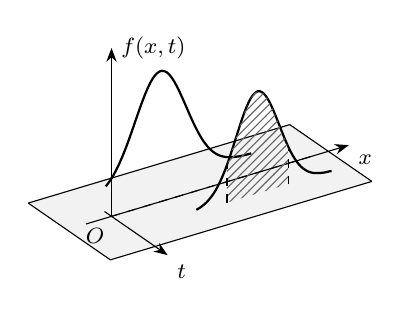
\begin{tikzpicture}[x=1cm,y=1cm,scale=1.62,every node/.style={font=\footnotesize}]
  \fill[black!5] (-0.653,0.104) -- (1.397,0.719) -- (2.041,0.274) -- (-0.009,-0.341) -- cycle;
  \draw[thin] (-0.653,0.104) -- (1.397,0.719);
  \draw[thin] (1.397,0.719) -- (2.041,0.274);
  \draw[thin] (2.041,0.274) -- (-0.009,-0.341);
  \draw[thin] (-0.009,-0.341) -- (-0.653,0.104);
  \draw[-{Stealth[length=5pt]}] (0,0) -- (0,1.32) node[right] {$f(x,t)$};
  \draw[-{Stealth[length=5pt]}] (-0.200,-0.060) -- (1.860,0.558) node[below right] {$x$};
  \draw[-{Stealth[length=5pt]}] (-0.055,0.038) -- (0.440,-0.304) node[below right] {$t$};
  \node[below left] at (0.02,-0.02) {$O$};
  \draw[thick] plot[smooth] coordinates {(-0.045,0.235) (-0.025,0.261) (-0.005,0.290) (0.015,0.323) (0.035,0.360) (0.055,0.400) (0.075,0.445) (0.095,0.493) (0.115,0.544) (0.135,0.598) (0.155,0.654) (0.175,0.712) (0.195,0.770) (0.215,0.827) (0.235,0.883) (0.255,0.936) (0.275,0.985) (0.295,1.029) (0.315,1.067) (0.335,1.098) (0.355,1.120) (0.375,1.135) (0.395,1.141) (0.415,1.138) (0.435,1.128) (0.455,1.109) (0.475,1.083) (0.495,1.051) (0.515,1.014) (0.535,0.973) (0.555,0.929) (0.575,0.884) (0.595,0.838) (0.615,0.792) (0.635,0.748) (0.655,0.706) (0.675,0.667) (0.695,0.631) (0.715,0.598) (0.735,0.570) (0.755,0.545) (0.775,0.524) (0.795,0.507) (0.815,0.493) (0.835,0.482) (0.855,0.474) (0.875,0.469) (0.895,0.465) (0.915,0.464) (0.935,0.464) (0.955,0.465) (0.975,0.467) (0.995,0.470) (1.015,0.474) (1.035,0.478) (1.055,0.483) (1.075,0.488) (1.095,0.494)};
  \draw[thick] plot[smooth] coordinates {(0.665,0.051) (0.685,0.063) (0.705,0.076) (0.725,0.092) (0.745,0.110) (0.765,0.132) (0.785,0.157) (0.805,0.186) (0.825,0.220) (0.845,0.259) (0.865,0.302) (0.885,0.350) (0.905,0.403) (0.925,0.460) (0.945,0.520) (0.965,0.583) (0.985,0.646) (1.005,0.708) (1.025,0.768) (1.045,0.823) (1.065,0.872) (1.085,0.914) (1.105,0.946) (1.125,0.968) (1.145,0.980) (1.165,0.980) (1.185,0.970) (1.205,0.950) (1.225,0.920) (1.245,0.883) (1.265,0.840) (1.285,0.792) (1.305,0.742) (1.325,0.691) (1.345,0.640) (1.365,0.592) (1.385,0.547) (1.405,0.506) (1.425,0.470) (1.445,0.439) (1.465,0.412) (1.485,0.390) (1.505,0.373) (1.525,0.360) (1.545,0.350) (1.565,0.344) (1.585,0.340) (1.605,0.339) (1.625,0.339) (1.645,0.341) (1.665,0.343) (1.685,0.347) (1.705,0.352) (1.725,0.356)};
  \fill[pattern=north east lines,pattern color=black!60] (0.905,0.108) -- (0.905,0.403) -- (0.925,0.460) -- (0.945,0.520) -- (0.965,0.583) -- (0.985,0.646) -- (1.005,0.708) -- (1.025,0.768) -- (1.045,0.823) -- (1.065,0.872) -- (1.085,0.914) -- (1.105,0.946) -- (1.125,0.968) -- (1.145,0.980) -- (1.165,0.980) -- (1.185,0.970) -- (1.205,0.950) -- (1.225,0.920) -- (1.245,0.883) -- (1.265,0.840) -- (1.285,0.792) -- (1.305,0.742) -- (1.325,0.691) -- (1.345,0.640) -- (1.365,0.592) -- (1.385,0.547) -- (1.385,0.252) -- cycle;
  \draw[dashed,thin] (0.905,0.108) -- (0.905,0.403);
  \draw[dashed,thin] (1.385,0.252) -- (1.385,0.547);
  \draw[dashed,thin] (0.000,0.000) -- (1.620,0.486);
\end{tikzpicture}
\captionof{figure}{一阶密度函数的平稳性示例}\label{fig:3.1}
\end{minipage}\hfill
\begin{minipage}[t]{0.50\linewidth}\centering
% 原书是三维示意：横轴 $t+\tau$、纵轴 $R(t+\tau,t)$、另有一条斜的 $t$ 轴；
% 两条曲线分别画在 $t=0$ 与 $t=a$ 两个平面上（后者沿 $t$ 轴抬高），
% 虚线示出两者的峰值等高、以及 $a$ 的平移。
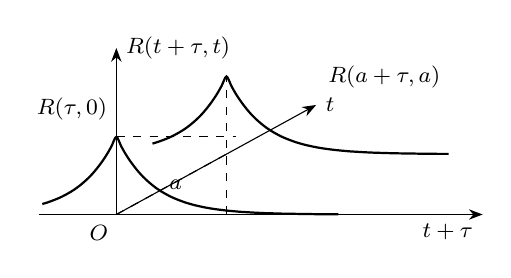
\begin{tikzpicture}[x=1cm,y=1cm,scale=0.94,every node/.style={font=\footnotesize}]
  \draw[-{Stealth[length=5pt]}] (-1.05,0) -- (4.95,0) node[below left] {$t+\tau$};
  \draw[-{Stealth[length=5pt]}] (0,0) -- (0,2.25) node[right] {$R(t+\tau,t)$};
  \draw[-{Stealth[length=5pt]}] (0,0) -- (2.70,1.48) node[right] {$t$};
  \node[below left] at (0.02,-0.02) {$O$};
  \fill[pattern=north east lines,pattern color=black!55] (-1.000,0) -- (-1.000,0.142) (-0.933,0.162) (-0.867,0.186) (-0.800,0.212) (-0.733,0.242) (-0.667,0.277) (-0.600,0.316) (-0.533,0.361) (-0.467,0.413) (-0.400,0.472) (-0.333,0.539) (-0.267,0.616) (-0.200,0.704) (-0.133,0.804) (-0.067,0.919) (0.000,1.050) (0.067,0.919) (0.133,0.804) (0.200,0.704) (0.267,0.616) (0.333,0.539) (0.400,0.472) (0.467,0.413) (0.533,0.361) (0.600,0.316) (0.667,0.277) (0.733,0.242) (0.800,0.212) (0.867,0.186) (0.933,0.162) (1.000,0.142) (1.067,0.124) (1.133,0.109) (1.200,0.095) (1.267,0.083) (1.333,0.073) (1.400,0.064) (1.467,0.056) (1.533,0.049) (1.600,0.043) (1.667,0.037) (1.733,0.033) (1.800,0.029) (1.867,0.025) (1.933,0.022) (2.000,0.019) (2.067,0.017) (2.133,0.015) (2.200,0.013) (2.267,0.011) (2.333,0.010) (2.400,0.009) (2.467,0.008) (2.533,0.007) (2.600,0.006) (2.667,0.005) (2.733,0.004) (2.800,0.004) (2.867,0.003) (2.933,0.003) (3.000,0.003) -- (3.000,0) -- cycle;
  \fill[pattern=north east lines,pattern color=black!55] (0.488,0.816) -- (0.488,0.958) (0.555,0.978) (0.621,1.002) (0.688,1.028) (0.755,1.058) (0.821,1.093) (0.888,1.132) (0.955,1.177) (1.021,1.229) (1.088,1.288) (1.155,1.355) (1.221,1.432) (1.288,1.520) (1.355,1.620) (1.421,1.735) (1.488,1.866) (1.555,1.735) (1.621,1.620) (1.688,1.520) (1.755,1.432) (1.821,1.355) (1.888,1.288) (1.955,1.229) (2.021,1.177) (2.088,1.132) (2.155,1.093) (2.221,1.058) (2.288,1.028) (2.355,1.002) (2.421,0.978) (2.488,0.958) (2.555,0.940) (2.621,0.925) (2.688,0.911) (2.755,0.899) (2.821,0.889) (2.888,0.880) (2.955,0.872) (3.021,0.865) (3.088,0.859) (3.155,0.853) (3.221,0.849) (3.288,0.845) (3.355,0.841) (3.421,0.838) (3.488,0.835) (3.555,0.833) (3.621,0.831) (3.688,0.829) (3.755,0.827) (3.821,0.826) (3.888,0.825) (3.955,0.824) (4.021,0.823) (4.088,0.822) (4.155,0.821) (4.221,0.820) (4.288,0.820) (4.355,0.819) (4.421,0.819) (4.488,0.819) -- (4.488,0.816) -- cycle;
  \draw[thick] plot[smooth] coordinates {(-1.000,0.142) (-0.933,0.162) (-0.867,0.186) (-0.800,0.212) (-0.733,0.242) (-0.667,0.277) (-0.600,0.316) (-0.533,0.361) (-0.467,0.413) (-0.400,0.472) (-0.333,0.539) (-0.267,0.616) (-0.200,0.704) (-0.133,0.804) (-0.067,0.919) (0.000,1.050) (0.067,0.919) (0.133,0.804) (0.200,0.704) (0.267,0.616) (0.333,0.539) (0.400,0.472) (0.467,0.413) (0.533,0.361) (0.600,0.316) (0.667,0.277) (0.733,0.242) (0.800,0.212) (0.867,0.186) (0.933,0.162) (1.000,0.142) (1.067,0.124) (1.133,0.109) (1.200,0.095) (1.267,0.083) (1.333,0.073) (1.400,0.064) (1.467,0.056) (1.533,0.049) (1.600,0.043) (1.667,0.037) (1.733,0.033) (1.800,0.029) (1.867,0.025) (1.933,0.022) (2.000,0.019) (2.067,0.017) (2.133,0.015) (2.200,0.013) (2.267,0.011) (2.333,0.010) (2.400,0.009) (2.467,0.008) (2.533,0.007) (2.600,0.006) (2.667,0.005) (2.733,0.004) (2.800,0.004) (2.867,0.003) (2.933,0.003) (3.000,0.003)};
  \draw[thick] plot[smooth] coordinates {(0.488,0.958) (0.555,0.978) (0.621,1.002) (0.688,1.028) (0.755,1.058) (0.821,1.093) (0.888,1.132) (0.955,1.177) (1.021,1.229) (1.088,1.288) (1.155,1.355) (1.221,1.432) (1.288,1.520) (1.355,1.620) (1.421,1.735) (1.488,1.866) (1.555,1.735) (1.621,1.620) (1.688,1.520) (1.755,1.432) (1.821,1.355) (1.888,1.288) (1.955,1.229) (2.021,1.177) (2.088,1.132) (2.155,1.093) (2.221,1.058) (2.288,1.028) (2.355,1.002) (2.421,0.978) (2.488,0.958) (2.555,0.940) (2.621,0.925) (2.688,0.911) (2.755,0.899) (2.821,0.889) (2.888,0.880) (2.955,0.872) (3.021,0.865) (3.088,0.859) (3.155,0.853) (3.221,0.849) (3.288,0.845) (3.355,0.841) (3.421,0.838) (3.488,0.835) (3.555,0.833) (3.621,0.831) (3.688,0.829) (3.755,0.827) (3.821,0.826) (3.888,0.825) (3.955,0.824) (4.021,0.823) (4.088,0.822) (4.155,0.821) (4.221,0.820) (4.288,0.820) (4.355,0.819) (4.421,0.819) (4.488,0.819)};
  \draw[dashed,thin] (0,0) -- (1.488,0.816);
  \draw[dashed,thin] (0,1.050) -- (1.62,1.050);
  \draw[dashed,thin] (1.488,0) -- (1.488,1.866);
  \node at (0.80,0.40) {$a$};
  \node[above] at (-0.60,1.14) {\footnotesize $R(\tau,0)$};
  \node at (3.62,1.86) {\footnotesize $R(a+\tau,a)$};
\end{tikzpicture}
\captionof{figure}{相关函数的平稳性示例}\label{fig:3.2}
\end{minipage}
\end{center}

严格平稳性要求全部统计特性都具有移动不变性\nobreak；而广义平稳性只要求一\nobreak、二阶矩特性具有移动不变性\nobreak。应用与研究最多的平稳信号是广义平稳信号\nobreak，严格平稳性因要求太“苛刻”\nobreak，而更多地用于理论研究中\nobreak。严格平稳性与广义平稳性之间有关系\nobreak：
\begin{equation}
\begin{tikzpicture}[x=1cm,y=1cm,every node/.style={font=\small},baseline=(current bounding box.center)]
  % 原书画的是两对**大括号/圆括号**里的"严格平稳过程""广义平稳过程"，不画方框
  \node (sss) at (0,0) {$\left(\begin{array}{c}\text{严格平稳}\\[2pt]\text{过程}\end{array}\right)$};
  \node (wss) at (7.2,0) {$\left(\begin{array}{c}\text{广义平稳}\\[2pt]\text{过程}\end{array}\right)$};
  \draw[-{Stealth[length=6pt]}] (1.45,0.30) -- node[above,font=\scriptsize,inner sep=1.5pt]{如果其均值与相关函数存在} (5.75,0.30);
  \draw[-{Stealth[length=6pt]}] (5.75,-0.30) -- node[below,font=\scriptsize,inner sep=1.5pt]{不一定是} (1.45,-0.30);
\end{tikzpicture}
\label{eq:3.3}
\end{equation}
上述关系式指出\nobreak，广义平稳信号通常不一定是严格平稳的\nobreak，但高斯信号是一个例外\nobreak，下面的定理证明了这点\nobreak。

\thm{定理 3.1} 广义平稳的高斯信号必定是严格平稳的\nobreak。

\textbf{证明\nobreak：}如果高斯信号 $X(t)$ 是广义平稳的\nobreak，则其均值为常数 $m$\nobreak，协方差满足平稳不变性\nobreak，即 $C(s,t)=C(s+\tau,t+\tau)$\nobreak。利用前面给出的高斯信号特征函数的展开形式\nobreak：
\[
\phi_{X_1X_2\cdots X_n}(v_1,\cdots,v_n;t_1,\cdots,t_n)=\exp\left\{\ju\sum_{k=1}^{n}mv_k-\frac{1}{2}\sum_{i=1}^{n}\sum_{k=1}^{n}C(t_i,t_k)v_iv_k\right\}
\]
显然\nobreak，对于任何 $\tau$\nobreak，有
\[
\resizebox{\linewidth}{!}{$\displaystyle
\phi_{X_1X_2\cdots X_n}(v_1,v_2,\cdots,v_n;t_1,t_2,\cdots,t_n)=\phi_{X_1X_2\cdots X_n}(v_1,v_2,\cdots,v_n;t_1+\tau,t_2+\tau,\cdots,t_n+\tau)$}
\]
因此\nobreak，该信号是严格平稳的\nobreak。

关于离散随机信号（或随机序列\nobreak）的平稳性问题\nobreak，其讨论是类似的\nobreak。只需要将连续时间变量 $t$ 换为离散时间 $n$ 就行了\nobreak。

\begin{examplebox}
\textbf{例3.1}\quad 假定高斯随机信号 $U(t)$ 的一维密度函数为
\[
f(u;t)=\frac{1}{\sqrt{2\pi}\sigma}\exp\left[-\frac{(u-a)^2}{2\sigma^2}\right]
\]
其中 $a$ 与 $\sigma$ 为常数\nobreak，而且 $U(t)$ 在不同的时刻彼此独立\nobreak。试分析其平稳性\nobreak。

\textbf{解\nobreak：}\quad 根据独立性\nobreak，$U(t)$ 的任意 $n$ 维密度函数为 $n$ 个一维密度函数之积\nobreak，即
\[
f(u_1,u_2,\cdots,u_n;t_1,t_2,\cdots,t_n)=\frac{1}{\left(\sqrt{2\pi}\sigma\right)^n}\exp\left(-\frac{1}{2\sigma^2}\sum_{i=1}^{n}(u_i-a)^2\right)
\]
该结果与各个参量 $t_i$ 本身无关\nobreak，也与这组参量的平移无关\nobreak。于是\nobreak，$U(t)$ 是严格平稳信号\nobreak。
\end{examplebox}

显然\nobreak，同分布的独立信号必定是严格平稳信号\nobreak。例如\nobreak，伯努利序列是严格平稳的\nobreak。

\begin{examplebox}
\textbf{例3.2}\quad 试说明 2.2 节各例的平稳性\nobreak。

\textbf{解\nobreak：}\quad 根据这些例子中各个信号的均值\nobreak、相关函数与概率特性\nobreak，容易得出\nobreak：
\begin{citemize}
\item \fw{1}伯努利信号是严格平稳信号\nobreak，也是广义平稳信号\nobreak；
\item \fw{2}随机正弦信号（该例的特定条件下\nobreak）是广义平稳信号\nobreak；又由于是高斯的\nobreak，因此是严格平稳的\nobreak。
\item \fw{3}半随机二进制传输信号与泊松信号都是非平稳的\nobreak。
\end{citemize}

\textbf{例3.3}\quad 讨论乘法调制输出信号\nobreak：实广义平稳随机信号 $X(t)$ 通过乘法调制器得到随机信号 $Y(t)=X(t)\cos(\omega_0t+\Theta)$\nobreak，其中\nobreak，振荡频率 $\omega_0$ 是确定量\nobreak，相位 $\Theta$ 是 $[-\pi,+\pi)$ 内均匀分布的随机变量\nobreak，$\Theta$ 与 $X(t)$ 统计独立\nobreak。试讨论 $Y(t)$ 的广义平稳性\nobreak。
% 原书此处是半开区间 [−π,+π)，闭合符号排成全角括号

\textbf{解\nobreak：}\quad 简单地讲\nobreak，调制就是将信号附加到某个正弦波上\nobreak，是通信等应用中的重要技术\nobreak。乘法调制器将信号与某个正弦波相乘\nobreak，使信号附加到正弦波的振幅上\nobreak。调制器输出信号的均值为
\[
\E[Y(t)]=\E[X(t)]\E[\cos(\omega_0t+\Theta)]=0
\]
相关函数为
\[
\resizebox{\linewidth}{!}{$\displaystyle
\begin{aligned}
\E[Y(t+\tau)Y(t)]&=\E[X(t+\tau)X(t)\cos(\omega_0t+\omega_0\tau+\Theta)\cos(\omega_0t+\Theta)]\\
&=\E[X(t+\tau)X(t)]\times\frac{1}{2}\E[\cos(\omega_0\tau)+\cos(2\omega_0t+2\Theta+\omega_0\tau)]\\
&=\frac{1}{2}R_X(\tau)\cos(\omega_0\tau)
\end{aligned}$}
\]
由于均值是常数且相关函数仅与 $\tau$ 有关\nobreak，因此 $Y(t)$ 是广义平稳的\nobreak。
\end{examplebox}

对于实际问题\nobreak，利用概率分布与密度函数或通过它们计算各种平均来判断信号的平稳性是困难的\nobreak。如果产生与影响随机信号的主要物理条件不随时间而改变\nobreak，那么通常可以认为此信号是平稳的\nobreak。电子与通信工程中所遇到的随机信号\nobreak，很多都可以认为是平稳随机信号\nobreak。例如\nobreak，考察电子线路的热噪声电压 $U(t)$\nobreak，这里温度是影响 $U(t)$ 特性的主要物理条件\nobreak。刚接通电源时\nobreak，由于温度还在不断上升\nobreak，因此 $U(t)$ 是非平稳的\nobreak；过一段时间后\nobreak，电路的温度将达到稳定状态\nobreak，$U(t)$ 可以认为是平稳的\nobreak。

凡是不满足平稳性定义的随机信号\nobreak，统称为非平稳信号\nobreak。应该说\nobreak，非平稳信号具有更为广泛与实际的意义\nobreak，平稳信号只是一种近似或特殊情况\nobreak。当非平稳信号的统计特性变化比较缓慢时\nobreak，在一个较短的时段内\nobreak，非平稳信号可以近似为平稳信号来处理\nobreak。语音信号是明显的非平稳信号\nobreak，研究表明\nobreak，在 $10\sim30$ ms 的时段上\nobreak，语音信号可以近似为平稳信号对待\nobreak。因此\nobreak，在语音的处理中\nobreak，人们普遍实施 $10\sim30$ ms 的分帧\nobreak，再采用平稳信号的处理技术解决有关问题\nobreak。

\subsection{联合平稳性}
在讨论多个随机信号时\nobreak，联合平稳性指其联合统计特性对参量（组\nobreak）具有移动不变性\nobreak。

% EQNUMBERS: 3.1, 3.2, 3.3
% FIGNUMBERS: 3.1, 3.2
% PAGES: 63-65

% =====================================================================
%  frag_B —— 书 p.66–68（PDF p.80–82）
%  内容：3.1.2 联合平稳性（定义3.3、定义3.4）、例3.4、
%        §3.2* 循环平稳性、§3.2.1 严格循环平稳性（定义3.5、定理3.2 及其证明）、
%        （3.6）循环平稳⇄平稳的并列示意（原书两端用**大圆括号**，不是圆角方框，照原样画）、
%        §3.2.2 广义循环平稳性（定义3.6、定理3.3 及其证明）、
%        例3.5、例3.6 题面（起笔，本片不闭合）
%  本片编号公式：(3.4)(3.5)(3.6)(3.7)(3.8)；图：无
%  灰底框：例3.4（p.66 0.295–0.439，页内闭合）；
%          例3.5（p.68 0.330–0.713，含“事实上…严格循环平稳的”整段）；
%          例3.6（p.68 0.844 起开框，**本片不闭合**，由 frag_C 继续写并在 p.69 闭合）
%  接缝：末尾停在 p.68 末句“…上均匀分布的”半句上（tight_seam B→C，
%        frag_C 从“随机变量，$D$ 与 $X(t)$ 统计独立…”续写）
% =====================================================================

\thm{定义 3.3} 联合严格平稳性定义为随机信号 $X(t)$ 与 $Y(t)$ 的任意 $(n+m)$ 阶联合分布函数满足下面公式\nobreak：
\[
% 原书该式两行、第二行以"="起头并与第一行左端对齐
\resizebox{\linewidth}{!}{$\displaystyle
\begin{aligned}
&F_{XY}(x_1,x_2,\cdots,x_n,y_1,y_2,\cdots,y_m;t_1,t_2,\cdots,t_n,s_1,s_2,\cdots,s_m)\\
&=F_{XY}(x_1,x_2,\cdots,x_n,y_1,y_2,\cdots,y_m;t_1+u,t_2+u,\cdots,t_n+u,s_1+u,s_2+u,\cdots,s_m+u)
\end{aligned}$}
\]
其中\nobreak，各个时间参量与状态的取值（在相应定义域中\nobreak）是任意的\nobreak。

上述定义可以改用 $X(t)$ 与 $Y(t)$ 的密度函数给出\nobreak。相似地\nobreak，联合严格平稳随机信号的分布\nobreak、密度函数与互相关函数只与两时刻的相对差 $\tau=t_1-t_2$ 有关\nobreak。同样\nobreak，联合广义平稳性只要求二阶联合矩对于参量组具有平移不变性\nobreak。

\thm{定义 3.4} 联合广义平稳性定义为 $X(t)$ 与 $Y(t)$ 分别是广义平稳的\nobreak，且满足下面公式\nobreak：
\[
R_{XY}(t_1,t_2)=R_{XY}(t+\tau,t)=R_{XY}(\tau),\qquad \tau=t_1-t_2
\]

\begin{examplebox}
\textbf{例3.4}\quad 讨论例 3.3 中乘法调制器的输入与输出信号的互相关函数与联合平稳性\nobreak。

\textbf{解\nobreak：}\quad 由例 3.3\nobreak，输入与输出信号各自广义平稳\nobreak，又互相关函数为
\[
% 原书如此：本行原书用 ω（不带下标 0），与例3.3 的 ω_0 不一致，照原样保留
\E[X(t+\tau)Y(t)]=\E[X(t+\tau)X(t)\cos(\omega t+\Theta)]=R_X(\tau)\E[\cos(\omega t+\Theta)]=0
\]
显然\nobreak，输入与输出信号是联合广义平稳的\nobreak，并且正交\nobreak。我们应该注意到\nobreak，在有关应用中如果振荡不是随机相位的\nobreak，则输出信号可能不是平稳的\nobreak，输入与输出信号不会正交\nobreak，也不会联合广义平稳\nobreak。
\end{examplebox}

% 原书本节标题为「3.2* 循环平稳性」，星号紧贴节号（表示选读）。
% 用导言区的 \ssection：只在本次调用内给 \thesection 补星号，出组复原，
% 故紧随其后的 \subsection 仍编为 3.2.1、3.2.2。
\ssection{循环平稳性}

随机过程如果不平稳\nobreak，则它的统计量是时变的\nobreak，当这种时变呈周期性时\nobreak，过程中通常蕴含着某种周期特征\nobreak。循环平稳性关注随机过程的统计特性上的周期性\nobreak。它分为严格循环平稳性与广义循环平稳性\nobreak。

\subsection{严格循环平稳性}
\thm{定义 3.5} 严格循环平稳性\fw{SSCS}定义为过程的任意 $n$ 阶概率分布函数具有下述的周期性
\begin{equation}
\resizebox{\dimexpr\linewidth-4em\relax}{!}{$\displaystyle
F(x_1,x_2,\cdots,x_n;t_1,t_2,\cdots,t_n)=F(x_1,x_2,\cdots,x_n;t_1+kT,t_2+kT,\cdots,t_n+kT)$}
\label{eq:3.4}
\end{equation}

式中\nobreak，$k$ 为任意整数\nobreak，$T$ 为正常数\nobreak。称 $T$ 为 $X(t)$ 的循环周期\nobreak。（注意\nobreak：这里的 $T$ 与我们常使用的参数集 $T$ 有不同的含义\nobreak）

严格循环平稳过程 $X(t)$ 具有如下特性\nobreak：
\begin{citemize}
\item ① 严格平稳过程可以看做严格循环平稳过程\nobreak，而其循环周期可以是任意值\nobreak。
\item ② 严格循环平稳过程通过在其循环周期内均匀滑动后\nobreak，变为严格平稳过程\nobreak。表述如下\nobreak。
\end{citemize}

\thm{定理 3.2} 若 $X(t)$ 是周期为 $T$ 的严格循环平稳过程\nobreak，$\Theta$ 是 $[0,T)$ 上均匀分布的独立随机变量\nobreak，则 $Y(t)=X(t-\Theta)$ 是严格平稳的\nobreak，且其任意 $n$ 维分布为
\begin{equation}
\resizebox{\dimexpr\linewidth-4em\relax}{!}{$\displaystyle
F_Y(y_1,y_2,\cdots,y_n;t_1,t_2,\cdots,t_n)=\frac{1}{T}\int_0^T F_X(y_1,y_2,\cdots,y_n;t_1-\theta,t_2-\theta,\cdots,t_n-\theta)\dif\theta$}
\label{eq:3.5}
\end{equation}

\textbf{证明\nobreak：}由定义并利用条件概率与全概率公式有
\[
\resizebox{\linewidth}{!}{$\displaystyle
f_Y(y_1,y_2,\cdots,y_n;t_1,t_2,\cdots,t_n)=\int_{-\infty}^{+\infty}f_{Y\mid\Theta}(y_1,y_2,\cdots,y_n;t_1,t_2,\cdots,t_n\mid\theta)f_\Theta(\theta)\dif\theta$}
\]
可以证明\nobreak，相仿的公式如下
\[
\resizebox{\linewidth}{!}{$\displaystyle
F_Y(y_1,y_2,\cdots,y_n;t_1,t_2,\cdots,t_n)=\int_{-\infty}^{+\infty}F_{Y\mid\Theta}(y_1,y_2,\cdots,y_n;t_1,t_2,\cdots,t_n\mid\theta)f_\Theta(\theta)\dif\theta$}
\]
由于 $\Theta$ 与 $X(t)$ 独立\nobreak，因此
\[
F_{Y\mid\Theta}(y_1,y_2,\cdots,y_n;t_1,t_2,\cdots,t_n\mid\theta)=P[X(t_1-\theta)\leqslant y_1,\cdots,X(t_n-\theta)\leqslant y_n]
\]
所以
\[
\resizebox{\linewidth}{!}{$\displaystyle
\begin{aligned}
F_Y(y_1,y_2,\cdots,y_n;t_1,t_2,\cdots,t_n)&=\int_0^T P[X(t_1-\theta)\leqslant y_1,\cdots,X(t_n-\theta)\leqslant y_n]\frac{1}{T}\dif\theta\\
&=\frac{1}{T}\int_0^T F_X(y_1,y_2,\cdots,y_n;t_1-\theta,t_2-\theta,\cdots,t_n-\theta)\dif\theta
\end{aligned}$}
\]
如果我们令观察时刻移动任意 $\tau$ 值
% 原书三行：第一行是左端，后两行以"="起头、与第一行左端对齐
\[
\begin{aligned}
&F_Y(y_1,y_2,\cdots,y_n;t_1+\tau,t_2+\tau,\cdots,t_n+\tau)\\
&=\frac{1}{T}\int_0^T F_X(y_1,y_2,\cdots,y_n;t_1-(\theta-\tau),t_2-(\theta-\tau),\cdots,t_n-(\theta-\tau))\dif\theta\\
&=\frac{1}{T}\int_{-\tau}^{T-\tau} F_X(y_1,y_2,\cdots,y_n;t_1-u,t_2-u,\cdots,t_n-u)\dif u
\end{aligned}
\]
利用 $F_X(\cdots)$ 关于各个参量是 $T$ 的周期函数有
\[
\resizebox{\linewidth}{!}{$\displaystyle
\begin{aligned}
F_Y(y_1,y_2,\cdots,y_n;t_1+\tau,t_2+\tau,\cdots,t_n+\tau)&=\frac{1}{T}\int_0^T F_X(y_1,y_2,\cdots,y_n;t_1-u,t_2-u,\cdots,t_n-u)\dif u\\
&=F_Y(y_1,y_2,\cdots,y_n;t_1,t_2,\cdots,t_n)
\end{aligned}$}
\]
可见\nobreak，$Y(t)=X(t-\Theta)$ 是严格平稳的\nobreak。

在实际应用中\nobreak，信号 $X(t)$ 经过传送发生时延\nobreak，变成 $Y(t)=X(t-\Theta)$\nobreak，其中时延 $\Theta$ 通常是随机的\nobreak，并可认为它服从 $[0,T)$ 上的均匀分布\nobreak，我们称这样的变化为随机滑动（或抖动\nobreak）\nobreak。循环平稳过程的统计特性以周期 $T$ 循环重复\nobreak，但在一个周期内一般是不一致的\nobreak。$[0,T)$ 上均匀的随机滑动\nobreak，使得周期内的不一致性消失\nobreak，统计特性不再随参数的移动而变化\nobreak，因而变成了平稳过程\nobreak。随机过程的平稳性与循环平稳性之间的关系可简述为
\begin{equation}
\begin{tikzpicture}[x=1cm,y=1cm,every node/.style={font=\small},baseline=(current bounding box.center)]
  \node (cyc) at (0,0) {$\left(\begin{array}{c}\text{循环平稳}\\[1pt]\text{过程}\end{array}\right)$};
  \node (sta) at (7.4,0) {$\left(\begin{array}{c}\text{平稳}\\[1pt]\text{过程}\end{array}\right)$};
  \draw[-{Stealth[length=6pt]}] (1.35,0.32) -- node[above,font=\scriptsize,inner sep=1.5pt]{经周期内独立\nobreak、均匀的随机滑动} (6.05,0.32);
  \draw[-{Stealth[length=6pt]}] (6.05,-0.32) -- node[below,font=\scriptsize,inner sep=1.5pt]{以任意值为周期} (1.35,-0.32);
\end{tikzpicture}
\label{eq:3.6}
\end{equation}
对于后面的广义循环平稳性\nobreak，相似的关系同样成立\nobreak。

\subsection{广义循环平稳性}
类似于广义平稳性\nobreak，随机信号的广义循环平稳性可以表述如下\nobreak。

\thm{定义 3.6} 广义循环平稳\fw{WSCS}性定义为过程的均值与相关函数具有下述的周期性
\begin{equation}
\left\{\begin{array}{l}
\E[X(t)]=\E[X(t+kT)]\text{\nobreak，即}\quad m(t)=m(t+kT)\\
R(t_1,t_2)=R(t_1+kT,t_2+kT)
\end{array}\right.
\label{eq:3.7}
\end{equation}

式中\nobreak，$k$ 为任意整数\nobreak，$T$ 为正常数\nobreak。称 $T$ 为 $X(t)$ 的循环周期\nobreak。

广义循环平稳过程通过在其循环周期内均匀的随机滑动\nobreak，变为广义平稳过程\nobreak。表述如下\nobreak。

\thm{定理 3.3} 若 $X(t)$ 是周期为 $T$ 的广义循环平稳过程\nobreak，$\Theta$ 是 $[0,T)$ 上均匀分布的独立随机变量\nobreak，则 $Y(t)=X(t-\Theta)$ 是广义平稳的\nobreak，且
\begin{equation}
m_Y=\frac{1}{T}\int_0^T m_X(t)\dif t,\quad R_Y(\tau)=\frac{1}{T}\int_0^T R_X(t+\tau,t)\dif t
\label{eq:3.8}
\end{equation}

\textbf{证明\nobreak：}首先计算 $Y(t)$ 的均值\nobreak。可运用条件均值\nobreak，并利用 $X(t)$ 与 $\Theta$ 统计独立\nobreak，有
\[
m_Y=\E[Y(t)]=\E\{\E[X(t-\Theta)\mid\Theta]\}=\E[m_X(t-\Theta)]=\int_0^T m_X(t-\theta)f_\Theta(\theta)\dif\theta
\]
考虑到 $m_X(t)$ 是周期为 $T$ 的函数\nobreak，而积分区间正好是 $T$\nobreak，有
\[
m_Y=\frac{1}{T}\int_0^T m_X(t-\theta)\dif\theta=\frac{1}{T}\int_0^T m_X(t)\dif t=\text{常数}
\]
对于相关函数\nobreak，同理可得
\[
\begin{aligned}
R_Y(t+\tau,t)&=\E\{\E[X(t+\tau-\Theta)X(t-\Theta)\mid\Theta]\}\\
&=\E[R_X(t+\tau-\Theta,t-\Theta)]=\frac{1}{T}\int_0^T R_X(t+\tau,t)\dif t
\end{aligned}
\]
积分对 $t$ 进行\nobreak，因此结果仅与 $\tau$ 有关\nobreak。于是 $Y(t)=X(t-\Theta)$ 是广义平稳的\nobreak。

\begin{examplebox}
\textbf{例3.5}\quad 半随机二进制传输过程 $X(t)$\nobreak，如前面 2.2 节所述\nobreak。讨论它的循环平稳性\nobreak。

\textbf{解\nobreak：}\quad 首先由 2.2 节的结果\nobreak，$X(t)$ 的均值 $m(t)=p-q$ 为常数\nobreak。又
\[
\begin{aligned}
R(t_1+kT,t_2+kT)&=4pq\delta\left(\left[(t_1+kT)/T\right]-\left[(t_2+kT)/T\right]\right)+1-4pq\\
&=4pq\delta\left(\left[t_1/T\right]-\left[t_2/T\right]+(k-k)\right)+1-4pq\\
&=R(t_1,t_2)
\end{aligned}
\]
因此\nobreak，$X(t)$ 是广义循环平稳过程\nobreak，但不是广义平稳过程\nobreak。

事实上\nobreak，半随机二进制传输过程 $X(t)$ 是严格循环平稳的\nobreak。因为\nobreak，对于任意 $n$ 维概率分布函数\nobreak，若取观察时刻组 $t_1,t_2,\cdots,t_n\in(-\infty,+\infty)$\nobreak，有
\[
\resizebox{\dimexpr\linewidth-2em\relax}{!}{$\displaystyle
F(x_1,x_2,\cdots,x_n;t_1,t_2,\cdots,t_n)=P[X(t_1)\leqslant x_1,X(t_2)\leqslant x_2,\cdots,X(t_n)\leqslant x_n]$}
\]
由于不同时隙上的取值彼此统计独立并具有相同的分布\nobreak，该联合事件的概率取决于观察时刻之间的相对关系\nobreak：哪些落在同一个传输时隙内\nobreak，哪些落在不同的传输时隙上\nobreak。如果时刻都移动一个时隙长度 $T$\nobreak，得到新的观察时刻组 $t_1+T,t_2+T,\cdots,t_n+T\in(-\infty,+\infty)$\nobreak，在新的时刻组里\nobreak，各时刻之间的上述关系保持不变\nobreak。于是\nobreak，联合事件的概率不变\nobreak，即
\[
\resizebox{\dimexpr\linewidth-2em\relax}{!}{$\displaystyle
\begin{aligned}
F(x_1,x_2,\cdots,x_n;t_1,t_2,\cdots,t_n)&=P[X(t_1+T)\leqslant x_1,X(t_2+T)\leqslant x_2,\cdots,X(t_n+T)\leqslant x_n]\\
&=F(x_1,x_2,\cdots,x_n;t_1+T,t_2+T,\cdots,t_n+T)
\end{aligned}$}
\]
所以\nobreak，$X(t)$ 是严格循环平稳的\nobreak。
\end{examplebox}

有趣的是\nobreak，由定义与图 2.7 可见\nobreak，半随机二进制传输过程的任何一个样本函数几乎必定不是周期的\nobreak，但这一过程却是循环平稳的\nobreak。这是因为该过程蕴含的周期特征是“潜在”的\nobreak，是统计意义上的\nobreak。周期特征的根源在于信号中时隙的划分\nobreak。在应用中\nobreak，这种“潜在”的周期信息也可以被利用起来进行信号分析\nobreak。循环平稳信号分析与循环统计量理论是现代信号分析理论的一个重要的部分\nobreak。

% ↓ 例3.6 的灰底框在此开框，**本片不闭合**（延续到书 p.69，由 frag_C 结尾闭合）
\begin{examplebox}
\textbf{例3.6}\quad 讨论乘法调制输出信号（续\nobreak）\nobreak。实广义平稳随机信号 $X(t)$ 通过乘法调制器得到随机信号 $Y(t)=X(t)\cos\omega_0t$\nobreak，其中\nobreak，振荡频率 $\omega_0$ 是确定量\nobreak。

\fw{1}试讨论 $Y(t)$ 的循环平稳性\nobreak。

\fw{2}经过 $[0,2\pi/\omega_0)$ 上的随机滑动后得到 $Z(t)=Y(t-D)$\nobreak，$D$ 是 $[0,2\pi/\omega_0)$ 上均匀分布的
% 注：原书两处区间都是半开的 [0,2π/ω_0)，右端是「)」不是「]」，已逐像素放大核对。
% 本行是全片最后一行，**故意的半句**（tight_seam B→C）；frag_C 从「随机变量，$D$ 与…」续写。
% （1）（2）的全角括号照原书写，未包 \fw，留给 fixparen.py 统一处理。
% EQNUMBERS: 3.4, 3.5, 3.6, 3.7, 3.8
% FIGNUMBERS: （无，本片没有插图）
% PAGES: 66-68
% =====================================================================
%  frag_C —— 书 p.69–71（PDF p.83–85）
%  内容：例3.6 框尾（本片第一行在 frag_B 打开的 examplebox 内）、
%        §3.3 平稳信号的相关函数、§3.3.1 基本性质（性质1 及其五点证明）、
%        图3.3（(a)–(e) 五个子图一排）、性质2、性质3、
%        §3.3.2 物理意义、性质4（(3.9)(3.10)(3.11)）
%  本片编号公式：(3.9)(3.10)(3.11)；图3.3
%  灰底框：例3.6 框尾（p.69 的 0.057–0.494，grey 判定），**本片是闭框方**，
%          只写一次 \end{examplebox}（frag_B 是开框方，不得在这里再开框）
%  接缝：B→C 是同段接缝（plan.json tight_seams），本片首行 = 例3.6 题面的后半句，
%        装配时与 frag_B 末行用单个换行接成同一段，**不要重复前半句**
%  末尾：p.71 页末"相关函数中所包含的各种参数如图 3.4 所示。"（图3.4 在 frag_D）
% =====================================================================
随机变量\nobreak，$D$ 与 $X(t)$ 统计独立\nobreak，试讨论 $Z(t)$ 的平稳性\nobreak。

\textbf{解\nobreak：}\quad\fw{1}均值与相关函数为
\[
m_Y(t)=\E[Y(t)]=\E[X(t)]\cos\omega_0t=m_X\cos\omega_0t
\]
\[
\begin{aligned}
R_Y(t+\tau,t)&=\E[X(t+\tau)\cos\omega_0(t+\tau)X(t)\cos\omega_0t]\\
&=R_X(\tau)\cos\omega_0(t+\tau)\cos\omega_0t\\
&=\frac{1}{2}R_X(\tau)\left[\cos\omega_0(2t+\tau)+\cos\omega_0\tau\right]
\end{aligned}
\]
显然\nobreak，$m_Y(t)$ 是周期为 $2\pi/\omega_0$ 的周期函数\nobreak，$R_Y(t+\tau,t)$ 关于 $t$ 是周期为 $\pi/\omega_0$ 的周期函数\nobreak，因此 $Y(t)$ 是循环平稳信号\nobreak，周期为 $2\pi/\omega_0$\nobreak。

\fw{2}经过 $[0,2\pi/\omega_0)$ 上均匀的随机滑动后\nobreak，由定理 3.3 可得
\[
Z(t)=Y(t-D)=X(t-D)\cos\omega_0(t-D)
\]
是广义平稳的\nobreak，并且
\[
m_Z=\frac{\omega_0}{2\pi}\int_0^{2\pi/\omega_0}m_X\cos\omega_0t\dif t=0
\]
\[
\resizebox{\linewidth}{!}{$\displaystyle
\begin{aligned}
R_Z(\tau)&=\frac{\omega_0}{2\pi}\int_0^{2\pi/\omega_0}\frac{1}{2}R_X(\tau)\left[\cos\omega_0(2t+\tau)+\cos\omega_0\tau\right]\dif t\\
&=\frac{1}{2}R_X(\tau)\left[\frac{\omega_0}{2\pi}\int_0^{2\pi/\omega_0}\cos\omega_0(2t+\tau)\dif t+\frac{\omega_0}{2\pi}\int_0^{2\pi/\omega_0}\cos\omega_0\tau\dif t\right]\\
&=\frac{1}{2}R_X(\tau)\cos\omega_0\tau
\end{aligned}$}
\]
\end{examplebox}

本例中考虑乘法调制器的结果信号为 $Y(t)=X(t)\cos\omega_0t$\nobreak，等效于认为正弦信号的参考时间能够与信号 $X(t)$ 对齐\nobreak，使其初相为零\nobreak。实际上\nobreak，正弦信号通常具有随机相位\nobreak，这时的情况如例 3.3\nobreak，正弦信号与 $X(t)$ 之间存在随机时延 $D$\nobreak，而 $D$ 在 $[0,2\pi/\omega_0)$ 上均匀分布\nobreak。

\section{平稳信号的相关函数}
人们最关心随机信号的一\nobreak、二阶矩特征\nobreak。当 $\{X(t),t\in T\}$ 是平稳信号时\nobreak，其均值是常数\nobreak，相关函数只与时间差 $\tau=t_1-t_2$ 有关\nobreak，因此各种性质可以简化\nobreak。本节介绍平稳信号相关函数的性质及其物理意义\nobreak。

\subsection{基本性质}
下面以连续型信号为例说明平稳随机信号相关函数的性质\nobreak，这些结论也同样适用于离散型信号（即随机序列\nobreak）\nobreak。

\thm{性质 1} 若 $\{X(t),t\in T\}$ 是实平稳信号\nobreak，则相关函数满足\nobreak：
\begin{citemize}
\item ① 是实偶函数\nobreak，即 $R(\tau)=R(-\tau)$\nobreak；
\item ② 在原点处非负并达到最大\nobreak，即 $\lvert R(\tau)\rvert\leqslant R(0)$\nobreak，$R(0)=\E[X^2(t)]\geqslant 0$\nobreak；
\item ③ 若 $R(\tau_1)=R(0)$\nobreak，$\tau_1\neq 0$\nobreak，则 $R(\tau)$ 是周期为 $\tau_1$ 的周期函数\nobreak，这时称 $X(t)$ 为周期平稳信号\nobreak；
\item ④ 若 $R(\tau_1)=R(\tau_2)=R(0)$\nobreak，$\tau_1\neq 0$\nobreak，$\tau_2\neq 0$\nobreak，且 $\tau_1$ 与 $\tau_2$ 是不公约的\nobreak，则 $R(\tau)$ 为常数\nobreak；
\item ⑤ 若 $R(\tau)$ 在原点处连续\nobreak，则它处处连续\nobreak。
\end{citemize}

\textbf{证明\nobreak：}
\begin{citemize}
\item ① 直接由定义可得
\[
R(-\tau)=\E\{X(t)X(t+\tau)\}=\E\{X(t+\tau)X(t)\}=R(\tau)
\]
\item ② 利用柯西-施瓦兹不等式\nobreak：$\lvert\E[ZW]\rvert^2\leqslant\E\left[\lvert Z\rvert^2\right]\E\left[\lvert W\rvert^2\right]$\nobreak，令 $Z=X(t_1)$\nobreak，$W=X(t_2)$\nobreak，有
\[
\lvert\E[X(t_1)X(t_2)]\rvert^2\leqslant\E\left[\lvert X(t_1)\rvert^2\right]\E\left[\lvert X(t_2)\rvert^2\right]=R^2(0)
\]
即 $\lvert R(\tau)\rvert\leqslant R(0)$\nobreak。
\item ③ 令 $Z=X(t+\tau+\tau_1)-X(t+\tau)$\nobreak，$W=X(t)$\nobreak，利用柯西-施瓦兹不等式有
\[
\resizebox{\linewidth}{!}{$\displaystyle
\left\{\E\left[\left(X(t+\tau+\tau_1)-X(t+\tau)\right)X(t)\right]\right\}^2\leqslant\E\left[\left(X(t+\tau+\tau_1)-X(t+\tau)\right)^2\right]\E\left[X^2(t)\right]$}
\]
简化后得到
\[
\left[R(\tau+\tau_1)-R(\tau)\right]^2\leqslant 2\left[R(0)-R(\tau_1)\right]R(0)
\]
所以\nobreak，当 $R(\tau_1)=R(0)$ 时\nobreak，上式左端只能等于零\nobreak。于是 $R(\tau+\tau_1)=R(\tau)$\nobreak，即 $R(\tau)$ 以 $\tau_1$ 为周期\nobreak。
\item ④ 根据③的结论\nobreak，$R(\tau)$ 既以 $\tau_1$ 为周期\nobreak，又以 $\tau_2$ 为周期\nobreak，而 $\tau_1$ 与 $\tau_2$ 是不公约的\nobreak，因此 $R(\tau)$ 只能是常数\nobreak。
\item ⑤ 令 $\tau_1=\Delta\tau$ 并利用上面结果得
\[
\left[R(\tau+\Delta\tau)-R(\tau)\right]^2\leqslant 2\left[R(0)-R(\Delta\tau)\right]R(0)
\]
令上式右端为 $B(\Delta\tau)$\nobreak，于是可得
\[
-\sqrt{B(\Delta\tau)}\leqslant R(\tau+\Delta\tau)-R(\tau)\leqslant\sqrt{B(\Delta\tau)}
\]
若 $R(\tau)$ 在原点处连续\nobreak，则 $R(0)$ 有界\nobreak，并且有 $\lim\limits_{\Delta\tau\to 0}\left[R(0)-R(\Delta\tau)\right]=0$\nobreak。于是可得
\[
\lim_{\Delta\tau\to 0}B(\Delta\tau)=0
\]
利用极限的性质有
\[
\lim_{\Delta\tau\to 0}\left[R(\tau+\Delta\tau)-R(\tau)\right]=0
\]
因此在 $\tau$ 的定义域中\nobreak，$R(\tau)$ 处处连续\nobreak。
\end{citemize}

相关函数的性质表明\nobreak，其曲线不能是任意形状的图形\nobreak。图~\ref{fig:3.3} 中列举了几个不可能作为 $R(\tau)$ 的例子\nobreak，其中图(a)\nobreak、(b)\nobreak、(c)分别违背了性质 1 中的③\nobreak、④与①项\nobreak，图(d)\nobreak、(e)分别违背了性质 1 中的②与⑤项\nobreak。

\begin{figure}[htbp]\centering
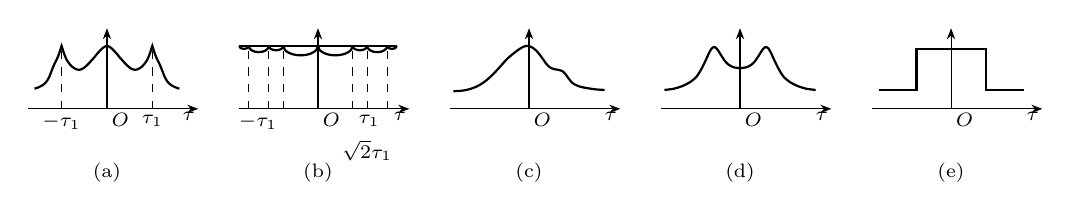
\begin{tikzpicture}[x=0.8cm,y=0.8cm,every node/.style={font=\scriptsize}]
% ---------------- (a) 三个等高的峰（违背性质1的③：R(tau_1)=R(0) 却非周期） ----------------
\begin{scope}
  \draw[-{Stealth[length=4pt]}] (-1.25,0) -- (1.45,0);
  \draw[-{Stealth[length=4pt]}] (0,0) -- (0,1.28);
  \node[below right,inner sep=1.5pt] at (0,0) {$O$};
  \node[below left,inner sep=1pt] at (1.45,0) {$\tau$};
  % 右半支，再镜像出左半支（保证严格对称、三峰等高）
  \draw[thick] plot[smooth] coordinates {
    (0.00,1.00) (0.04,0.985) (0.08,0.955) (0.12,0.915) (0.16,0.87)
    (0.20,0.82) (0.24,0.775) (0.28,0.73) (0.32,0.69) (0.36,0.655)
    (0.40,0.63) (0.44,0.62) (0.48,0.625) (0.52,0.645) (0.56,0.675)
    (0.60,0.72) (0.64,0.78) (0.67,0.85) (0.695,0.92) (0.71,0.97)
    (0.72,1.00) (0.73,0.97) (0.745,0.92) (0.77,0.85) (0.80,0.78)
    (0.84,0.70) (0.88,0.60) (0.92,0.50) (0.97,0.42) (1.03,0.37)
    (1.09,0.34) (1.15,0.32)};
  \draw[thick,xscale=-1] plot[smooth] coordinates {
    (0.00,1.00) (0.04,0.985) (0.08,0.955) (0.12,0.915) (0.16,0.87)
    (0.20,0.82) (0.24,0.775) (0.28,0.73) (0.32,0.69) (0.36,0.655)
    (0.40,0.63) (0.44,0.62) (0.48,0.625) (0.52,0.645) (0.56,0.675)
    (0.60,0.72) (0.64,0.78) (0.67,0.85) (0.695,0.92) (0.71,0.97)
    (0.72,1.00) (0.73,0.97) (0.745,0.92) (0.77,0.85) (0.80,0.78)
    (0.84,0.70) (0.88,0.60) (0.92,0.50) (0.97,0.42) (1.03,0.37)
    (1.09,0.34) (1.15,0.32)};
  \draw[dashed,thin] (-0.72,0) -- (-0.72,1.00);
  \draw[dashed,thin] (0.72,0) -- (0.72,1.00);
  \node[below,inner sep=2pt] at (-0.72,0) {$-\tau_1$};
  \node[below,inner sep=2pt] at (0.72,0) {$\tau_1$};
  \node at (0,-1.02) {(a)};
\end{scope}
% ---------------- (b) 平顶＋扇贝形起伏（违背④：τ1 与 √2τ1 不公约） ----------------
\begin{scope}[shift={(3.35,0)}]
  \draw[-{Stealth[length=4pt]}] (-1.25,0) -- (1.45,0);
  \draw[-{Stealth[length=4pt]}] (0,0) -- (0,1.28);
  \node[below right,inner sep=1.5pt] at (0,0) {$O$};
  \node[below left,inner sep=1pt] at (1.45,0) {$\tau$};
  % 平顶：R(tau) 恒等于 R(0) 的水平线
  \draw[thick] (-1.25,1.00) -- (1.25,1.00);
  % 顶线之下的扇贝形起伏：每两个切点之间一段上开口的弧
  \draw[thick] (-1.25,1.00) arc[start angle=180,end angle=360,x radius=0.075,y radius=0.05];
  \draw[thick] (-1.10,1.00) arc[start angle=180,end angle=360,x radius=0.16,y radius=0.10];
  \draw[thick] (-0.78,1.00) arc[start angle=180,end angle=360,x radius=0.115,y radius=0.07];
  \draw[thick] (-0.55,1.00) arc[start angle=180,end angle=360,x radius=0.275,y radius=0.15];
  \draw[thick] (0.00,1.00) arc[start angle=180,end angle=360,x radius=0.275,y radius=0.15];
  \draw[thick] (0.55,1.00) arc[start angle=180,end angle=360,x radius=0.115,y radius=0.07];
  \draw[thick] (0.78,1.00) arc[start angle=180,end angle=360,x radius=0.16,y radius=0.10];
  \draw[thick] (1.10,1.00) arc[start angle=180,end angle=360,x radius=0.075,y radius=0.05];
  % 自顶线到横轴的虚线
  \foreach \xx in {-1.10,-0.78,-0.55,0.55,0.78,1.10}{
    \draw[dashed,thin] (\xx,0) -- (\xx,1.00);}
  % 与原点标注 O 拉开距离：两个 tau1 标注改为左/右对齐各自的虚线
  \node[below left,inner sep=2pt] at (-0.55,0) {$-\tau_1$};
  \node[below right,inner sep=2pt] at (0.55,0) {$\tau_1$};
  % 原书 τ1 与 √2τ1 两个标注紧邻、会重叠；这里把 √2τ1 下移一行
  \node[below,inner sep=2pt] at (0.78,-0.40) {$\sqrt{2}\tau_1$};
  \node at (0,-1.02) {(b)};
\end{scope}
% ---------------- (c) 单峰但左右不对称（违背①：非实偶函数） ----------------
\begin{scope}[shift={(6.70,0)}]
  \draw[-{Stealth[length=4pt]}] (-1.25,0) -- (1.45,0);
  \draw[-{Stealth[length=4pt]}] (0,0) -- (0,1.28);
  \node[below right,inner sep=1.5pt] at (0,0) {$O$};
  \node[below left,inner sep=1pt] at (1.45,0) {$\tau$};
  \draw[thick] plot[smooth] coordinates {
    (-1.20,0.28) (-1.05,0.29) (-0.92,0.32) (-0.80,0.37) (-0.68,0.45)
    (-0.56,0.56) (-0.45,0.68) (-0.34,0.80) (-0.22,0.90) (-0.12,0.97)
    (-0.04,1.00) (0.04,0.98) (0.12,0.92) (0.20,0.82) (0.27,0.72)
    (0.33,0.66) (0.40,0.63) (0.47,0.62) (0.53,0.60) (0.58,0.55)
    (0.63,0.48) (0.68,0.42) (0.74,0.38) (0.82,0.35) (0.92,0.33)
    (1.05,0.31) (1.20,0.30)};
  \node at (0,-1.02) {(c)};
\end{scope}
% ---------------- (d) τ=0 处为极小（违背②：原点不是最大） ----------------
\begin{scope}[shift={(10.05,0)}]
  \draw[-{Stealth[length=4pt]}] (-1.25,0) -- (1.45,0);
  \draw[-{Stealth[length=4pt]}] (0,0) -- (0,1.28);
  \node[below right,inner sep=1.5pt] at (0,0) {$O$};
  \node[below left,inner sep=1pt] at (1.45,0) {$\tau$};
  \draw[thick] plot[smooth] coordinates {
    (0.00,0.645) (0.10,0.66) (0.18,0.70) (0.24,0.76) (0.30,0.85)
    (0.35,0.93) (0.40,0.98) (0.45,0.96) (0.50,0.87) (0.55,0.76)
    (0.62,0.62) (0.70,0.50) (0.80,0.42) (0.92,0.36) (1.05,0.32)
    (1.20,0.30)};
  \draw[thick,xscale=-1] plot[smooth] coordinates {
    (0.00,0.645) (0.10,0.66) (0.18,0.70) (0.24,0.76) (0.30,0.85)
    (0.35,0.93) (0.40,0.98) (0.45,0.96) (0.50,0.87) (0.55,0.76)
    (0.62,0.62) (0.70,0.50) (0.80,0.42) (0.92,0.36) (1.05,0.32)
    (1.20,0.30)};
  \node at (0,-1.02) {(d)};
\end{scope}
% ---------------- (e) 平顶方波（违背⑤：原点连续而别处不连续） ----------------
\begin{scope}[shift={(13.40,0)}]
  \draw[-{Stealth[length=4pt]}] (-1.25,0) -- (1.45,0);
  \draw[-{Stealth[length=4pt]}] (0,0) -- (0,1.28);
  \node[below right,inner sep=1.5pt] at (0,0) {$O$};
  \node[below left,inner sep=1pt] at (1.45,0) {$\tau$};
  \draw[thick] (-1.15,0.30) -- (-0.55,0.30) -- (-0.55,0.95)
               -- (0.55,0.95) -- (0.55,0.30) -- (1.15,0.30);
  \node at (0,-1.02) {(e)};
\end{scope}
\end{tikzpicture}
\caption{不可能作为 $R(\tau)$ 的函数图形的例子}\label{fig:3.3}
\end{figure}

根据相关函数与协方差函数的定义与性质\nobreak，还容易得到\nobreak：

\thm{性质 2} 若 $\{X(t),t\in T\}$ 是平稳信号\nobreak，则
\[
C(\tau)=R(\tau)-m^2\text{\nobreak，}\quad\sigma^2=R(0)-m^2
\]

\thm{性质 3} 若 $\{X(t),t\in T\}$ 与 $\{Y(t),t\in T\}$ 是联合平稳信号\nobreak，则
\[
R_{XY}(-\tau)=R_{YX}(\tau)\text{\nobreak，}\quad C_{XY}(\tau)=R_{XY}(\tau)-m_Xm_Y
\]

性质 2 和 3 显示出均值 $m_X$ 与自相关函数 $R_X(\tau)$ 在研究单个信号时的核心作用\nobreak，以及均值与互相关函数 $R_{XY}(\tau)$ 在研究两个信号时的核心作用\nobreak。因为有了它们\nobreak，信号的方差\nobreak、标准差\nobreak、均方值\nobreak、协方差\nobreak、相关系数等其他一\nobreak、二阶数字特征就完全确定了\nobreak。其实\nobreak，协方差函数与相关系数分别是原信号经过中心化与归一化以后的自相关函数\nobreak。因此\nobreak，关于相关函数的性质也同样适用于它们\nobreak。

\subsection{物理意义}
下面考察相关函数的物理意义\nobreak。相关函数反映随机信号在统计意义上的关联程度\nobreak。自相关函数度量信号自身在不同时刻之间的内在关联性\nobreak；而互相关函数度量不同信号之间的相互关联性\nobreak。粗略地讲\nobreak，无关与线性相关是这种关联性的两个极端\nobreak。相关的直观概念与它的通俗含义是基本相符的\nobreak，例如\nobreak，“子女的身高与他们父母的身高是相关的”\nobreak，“吸烟与肺癌是相关的”\nobreak，等等\nobreak。这些说法并不意味着每一个高个子的孩子都有高个子的父母\nobreak，每一个吸烟者都必定会患上肺癌\nobreak。相关是一种统计意义上的关联\nobreak，是大量同类事件总的关联趋势\nobreak。

对于平稳信号\nobreak，这种关联性只与被度量的两点间的距离有关\nobreak，而与从什么位置开始度量没有关系\nobreak。实际应用中\nobreak，我们注意到下面几个特点\nobreak：
\begin{citemize}
\item ① 如果信号 $X(t)$ 中含有平均分量（均值\nobreak）\nobreak，那么 $R(\tau)$ 将含有固定分量\nobreak。关系式 $R(\tau)=C(\tau)+m^2$ 就说明了这一点\nobreak。
\item ② 如果信号 $X(t)$ 含有周期分量\nobreak，那么 $R(\tau)$ 将含有同样周期的周期分量\nobreak。这种周期平稳信号的周期特性可说明如下\nobreak：
\[
\resizebox{\linewidth}{!}{$\displaystyle
\begin{aligned}
\E\left\{\left[X(t+nT)-X(t)\right]^2\right\}
&=R(t+nT,t+nT)-R(t+nT,t)-R(t,t+nT)+R(t,t)\\
&=R(0)-R(nT)-R(-nT)+R(0)\\
&=2\left[R(0)-R(nT)\right]
\end{aligned}$}
\]
\end{citemize}

可见\nobreak，$\E\left\{\left[X(t+nT)-X(t)\right]^2\right\}=0$ 等价于 $\left[R(0)-R(nT)\right]=0$\nobreak，即“信号依均方意义（也依概率为 1\nobreak）呈现周期性”的充要条件是“$R(\tau)$ 是周期函数”\nobreak，所以这种信号称为周期平稳信号\nobreak。

正弦随机信号 $X(t)=A\cos(\omega_0t+\Theta)$ 是一个典型的周期平稳信号\nobreak，$R(\tau)=\frac{1}{2}E\left(A^2\right)\cos(\omega_0\tau)$\nobreak，可见\nobreak，信号及其相关函数均是周期函数\nobreak。

\begin{citemize}
\item ③ 如果信号 $X(t)$ 中不含有任何周期分量\nobreak，那么\nobreak，从物理意义上看\nobreak，随机变量 $X(t_1)$ 与 $X(t_2)$ 的关联程度会随着间距的增大而逐渐减小\nobreak，直至无关\nobreak。对于两个不同的信号 $X(t)$ 与 $Y(t)$\nobreak，也有相似的特性\nobreak。虽然从严格的数学理论上讲\nobreak，并非所有的平稳过程都满足这种特性\nobreak，但我们仍然给出下面的性质\nobreak，它适用于大多数的实际信号\nobreak。
\end{citemize}

\thm{性质 4} 实际应用中的非周期平稳信号\nobreak，一般都满足
\begin{equation}
\lim_{\tau\to\infty}C(\tau)=0\text{\nobreak，}\quad\lim_{\tau\to\infty}C_{XY}(\tau)=0
\label{eq:3.9}
\end{equation}
它们等价于
\begin{equation}
\lim_{\tau\to\infty}R(\tau)=m^2\text{\nobreak，}\quad\lim_{\tau\to\infty}R_{XY}(\tau)=m_Xm_Y
\label{eq:3.10}
\end{equation}
可见\nobreak，在平稳信号的应用研究中\nobreak，相关函数 $R(\tau)$ 是最主要的统计表征\nobreak。有了它就获得了信号的其他主要参数\nobreak：
\begin{equation}
m^2=R(\infty)\text{\nobreak，}\quad\E[X^2(t)]=R(0)\text{\nobreak，}\quad\sigma^2=C(0)=R(0)-R(\infty)
\label{eq:3.11}
\end{equation}
相关函数中所包含的各种参数如图 3.4 所示\nobreak。

% EQNUMBERS: 3.9, 3.10, 3.11
% FIGNUMBERS: 3.3
% PAGES: 69-71

% =====================================================================
%  frag_D —— 书 p.72–74（PDF p.86–88）
%  内容：§3.3.2 第④条（相关系数与相关时间）、式(3.12)、例3.7、
%        §3.4 功率谱密度与互功率谱密度、3.4.1 基本概念、定理3.4（维纳-辛钦定理）、
%        3.4.2 定义与性质、1. 功率谱密度、定义3.7、(3.17)(3.18)(3.19)、
%        例3.8、三个无编号傅里叶变换式、图3.6/图3.7
%  本片编号公式：(3.12)(3.13)(3.14)(3.15)(3.16)(3.17)(3.18)(3.19)
%  图：图3.4+图3.5（p72 中部，并排）、图3.6+图3.7（p74 下部，并排）
%  灰底框：例3.7（p72 0.444–0.737，单页内开闭）、例3.8（p74 0.447–0.544，单页内开闭）
%  接缝：
%    · 首行即 p72 首行（④ 起头的段落）。扫描页判读：④ 首行缩进 2 字、
%      续行回到版心左边界（与 p71 的 ①②③ 完全一致，原书这些条目**没有悬挂缩进**）。
%      因 CH3_SPEC §4 规定 ①②③④ 条目用 citemize，且 frag_A 对同类条目亦用 citemize，
%      此处仍用 citemize。⚠ frag_C 必须在 ③ 那段之后就**闭合**它自己的 citemize
%      （性质 4 与 (3.9)(3.10)(3.11) 不能在列表内），④ 由本片另起一个新列表。
%      若主转录者决定 ④ 用普通段落，只需删掉本片 ④ 前后的
%      \begin{citemize} / \item / \end{citemize} 三行。
%    · 末行即 p74 页末"…为其相关函数的傅里叶变换，即"，**停在这里**；
%      D→E 是同段接缝，frag_E 从 p75 的无编号式（与 (3.16) 并行的相关函数—功率谱对）
%      续写。
% =====================================================================

% ---- 以下为 §3.3.2 的第 ④ 条（接 p71 的 ①②③） ----
\begin{citemize}
\item ④ 更为统一与准确地度量关联性可以使用相关系数 $\rho(\tau)$ 与互相关系数 $\rho_{XY}(\tau)$\nobreak，因为它们“排除”了均值与方差的影响\nobreak。由于 $\rho(\tau)$ 是 $X(t)$ 的归一化信号的自相关函数\nobreak，容易知道\nobreak，$\lvert\rho(\tau)\rvert\leqslant\rho(0)=1$\nobreak。$\rho(0)=1$表明在相同时刻处关联性总是达到满值 1\nobreak。
\end{citemize}

在实际工程中\nobreak，当 $\tau$ 大于某个值以后\nobreak，$\rho(\tau)$ 就很小了\nobreak。不妨确定一个粗略的时间值 $\tau_0$\nobreak，以它作为相关与否的简单分界点\nobreak。为此\nobreak，我们定义相关时间\fw{Corre-lation Time}$\tau_0$\nobreak，
% 原书如此：“Corre-lation”带连字符（疑为排版断词残留），照原样保留
使得 $\tau\geqslant\tau_0$ 以后\nobreak，$\lvert\rho(\tau)\rvert\leqslant\rho_0$\nobreak，其中 $\rho_0$ 是相关与否的门限\nobreak，通常定为 0.05\nobreak，如图 3.5 所示\nobreak。

\begin{center}
\begin{minipage}[t]{0.47\linewidth}\centering
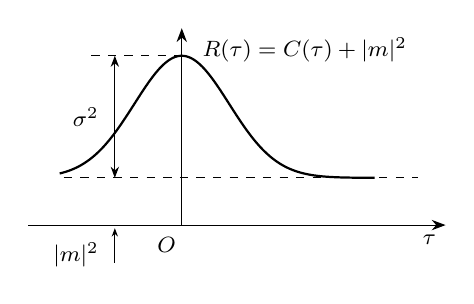
\begin{tikzpicture}[x=1cm,y=1cm,every node/.style={font=\footnotesize}]
  % 坐标轴
  \draw[-{Stealth[length=5pt]}] (-1.95,0) -- (3.35,0) node[below left] {$\tau$};
  \draw[-{Stealth[length=5pt]}] (0,0) -- (0,2.50);
  \node[below left] at (0.05,-0.03) {$O$};
  % 相关函数曲线 R(tau)=C(tau)+|m|^2
  \draw[thick] plot[domain=-1.55:2.45,samples=140] (\x,{0.60+1.55*exp(-(\x/0.85)^2)});
  % 峰值处虚线（上）与 |m|^2 处虚线（下）
  \draw[dashed,thin] (-1.15,2.15) -- (0,2.15);
  \draw[dashed,thin] (-1.50,0.60) -- (3.00,0.60);
  % sigma^2：两条虚线之间的双箭头
  \draw[{Stealth[length=4pt]}-{Stealth[length=4pt]},thin] (-0.85,0.60) -- (-0.85,2.15);
  \node[left] at (-0.93,1.37) {$\sigma^2$};
  % |m|^2：轴下方的小箭头（原书如此，箭头指到 tau 轴）
  \draw[-{Stealth[length=3pt]},thin] (-0.85,-0.48) -- (-0.85,-0.04);
  \node[left] at (-0.93,-0.38) {$\lvert m\rvert^2$};
  % 纵轴标注
  \node[right] at (0.14,2.22) {$R(\tau)=C(\tau)+\lvert m\rvert^2$};
\end{tikzpicture}
\captionof{figure}{相关函数}\label{fig:3.4}
\end{minipage}\hfill
\begin{minipage}[t]{0.50\linewidth}\centering
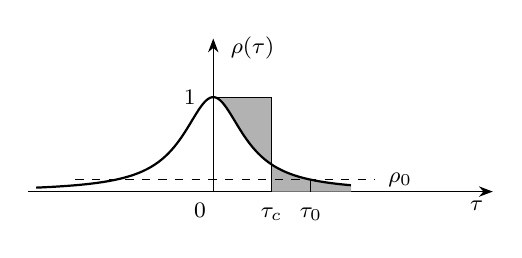
\begin{tikzpicture}[x=1cm,y=1.20cm,every node/.style={font=\footnotesize}]
  % 坐标轴
  \draw[-{Stealth[length=5pt]}] (-2.35,0) -- (3.55,0) node[below left] {$\tau$};
  \draw[-{Stealth[length=5pt]}] (0,0) -- (0,1.62);
  \node[right] at (0.10,1.52) {$\rho(\tau)$};
  \node[below left] at (0.03,-0.02) {$0$};
  % 阴影区一：y=1 与曲线之间，tau 在 [0,tau_c]
  \fill[black!30] (0,1) -- (0.74,1) -- plot[domain=0.74:0,samples=60] (\x,{1/(1+(\x/0.47)^2)}) -- cycle;
  % 阴影区二：tau_c 之后曲线下方的面积
  \fill[black!30] (0.74,0) -- plot[domain=0.74:1.75,samples=60] (\x,{1/(1+(\x/0.47)^2)}) -- (1.75,0) -- cycle;
  % 相关系数曲线
  \draw[thick] plot[domain=-2.25:1.75,samples=160] (\x,{1/(1+(\x/0.47)^2)});
  % 矩形等效：顶部水平边 + tau_c 竖线
  \draw[thin] (0,1) -- (0.74,1);
  \draw[thin] (0.74,0) -- (0.74,1);
  % rho_0 虚线与 tau_0 竖线
  \draw[dashed,thin] (-1.75,0.126) -- (2.05,0.126);
  \node[right] at (2.10,0.126) {$\rho_0$};
  \draw[thin] (1.24,0) -- (1.24,0.126);
  % 刻度标注
  \node[left] at (-0.10,1.00) {$1$};
  \node[below] at (0.74,-0.07) {$\tau_c$};
  \node[below] at (1.24,-0.07) {$\tau_0$};
\end{tikzpicture}
\captionof{figure}{相关系数与相关时间}\label{fig:3.5}
\end{minipage}
\end{center}

有时也用矩形等效形式来定义相关时间\nobreak，即
\begin{equation}
\tau_c=\int_0^{+\infty}\rho(\tau)\dif\tau
\label{eq:3.12}
\end{equation}
$\tau_0$ 与 $\tau_c$ 一般不相等\nobreak，但它们都示出了相关性有无的大致分界处\nobreak。

\begin{examplebox}
\textbf{例3.7}\quad 工程应用中某一平稳信号 $X(t)$ 的自相关函数为
\[
R_X(\tau)=100\eu^{-10\lvert\tau\rvert}+100\cos10\tau+100
\]
试估计其均值\nobreak、均方值和方差\nobreak。

\textbf{解\nobreak：}实际应用中\nobreak，具有这类自相关函数的信号 $X(t)$\nobreak，通常可以被视为两个平稳随机信号 $U(t)$ 与 $V(t)$ 的和\nobreak，而 $U(t)$ 与 $V(t)$ 的自相关函数分别为
\[
R_U(\tau)=100\eu^{-10\lvert\tau\rvert}+100\text{\nobreak，}\ R_V(\tau)=100\cos10\tau
\]
$U(t)$ 是 $X(t)$ 的非周期分量\nobreak，利用性质 4 可得
\[
m_U=\pm\sqrt{R_U(\infty)}=\pm10
\]
$V(t)$ 是周期分量\nobreak，很可能是具有随机相位的正弦信号的相关函数\nobreak，可以认为此分量的均值 $m_V=0$\nobreak。于是可得 $X(t)$ 的均值\nobreak、均方值和方差分别为
% 该式天然宽约 \linewidth+22pt（11pt 字号大于原书），按先例用 \resizebox 压到版心内
\[
\resizebox{\linewidth}{!}{$\displaystyle
m_X=m_U+m_V=\pm10\text{\nobreak，}\ \E\left[X^2(t)\right]=R_X(0)=300\text{\nobreak，}\ \sigma_X^2=R_X(0)-m_X^2=200$}
\]
\end{examplebox}

本例题说明了一种在已知条件不够充分时的工程分析方法\nobreak，尽管从理论上讲\nobreak，其中有的假设是不够严格的\nobreak，但它们合乎大多数的实际场合\nobreak，因此是很有用的\nobreak。

\section{功率谱密度与互功率谱密度}
功率是信号的重要物理量\nobreak，功率谱密度是功率沿频率轴的密度函数\nobreak。本节说明平稳随机信号的功率谱密度正好是它的自相关函数的傅里叶变换\nobreak，而且\nobreak，平稳随机信号的频域分析主要是考察它的功率谱与互功率谱\nobreak。

\subsection{基本概念}
在信号分析中\nobreak，信号的能量与功率分别被定义为
\[
E=\int_{-\infty}^{+\infty}x^2(t)\dif t\text{\nobreak，}\ P=\lim_{T\to\infty}\frac{1}{2T}\int_{-T}^{T}x^2(t)\dif t
\]
它们的物理意义可这样来理解\nobreak：假设 $x(t)$ 是电路中的电流或电压信号\nobreak，那么\nobreak，$E$ 与 $P$ 就分别是消耗在单位\fw{$1\,\Omega$}电阻上的能量或功率\nobreak。显然\nobreak，信号有两种类型\nobreak：能量型信号\nobreak，它的 $E$ 有限\nobreak，而 $P$ 为 0\nobreak；功率型信号\nobreak，它的 $P$ 有限\nobreak，而 $E$ 为无穷\nobreak。对于不同的信号类型我们应该研究不同的量\nobreak。

傅里叶变换的理论指出\nobreak，信号由各种频率成分构成\nobreak。信号 $x(t)$ 的傅里叶变换 $X(\ju\omega)$ 称为频谱密度\nobreak，简称频谱\nobreak，其含义是角频率为 $\omega$ 的成分在信号中所占的比例\nobreak。类似地\nobreak，可以分别为能量型与功率型信号定义能量谱密度或功率谱密度\nobreak，从信号的能量或功率沿 $\omega$ 轴的分布状况考察信号的频域特性\nobreak。

应用于随机信号时\nobreak，我们首先考虑某个样本函数的情形\nobreak，而后\nobreak，对这个结果进行统计平均\nobreak。设随机信号 $X(t)$ 的样本函数为 $X(t,\xi)$\nobreak，其样本功率定义为
\begin{equation}
P_s(\xi)=\lim_{T\to\infty}\frac{1}{2T}\int_{-T}^{T}X^2(t,\xi)\dif t
\label{eq:3.13}
\end{equation}
其中\nobreak，下标 s 表示它们基于样本函数\nobreak，$\xi$ 突出了样本功率的随机特性\nobreak，在不发生混淆时\nobreak，$\xi$ 也常常省略\nobreak。由于书写上时域与频域形式都采用了大写字母\nobreak，请注意根据各自的自变量来区分\nobreak。

随机信号的功率定义为
\begin{equation}
P=\E[P_s]=\lim_{T\to\infty}\frac{1}{2T}\int_{-T}^{T}\E[X^2(t)]\dif t=\lim_{T\to\infty}\frac{1}{2T}\int_{-T}^{T}R(t,t)\dif t
\label{eq:3.14}
\end{equation}
易见\nobreak，随机信号的功率可如下计算
\[
P=\Acal[R(t,t)]
\]
其中\nobreak，记算术平均算子为
\begin{equation}
\Acal[\ ]=\lim_{T\to\infty}\frac{1}{2T}\int_{-T}^{T}[\ ]\dif t
\label{eq:3.15}
\end{equation}
以后的讨论中\nobreak，我们主要关注平稳信号的情况\nobreak。这时 $R(t,t)=R(0)$ 是常量\nobreak，因此\nobreak，平稳信号的功率就是其均方值\nobreak，即 $P=\Acal[R(0)]=R(0)$\nobreak。正常情况下\nobreak，它是大于零的\nobreak，所以\nobreak，平稳信号都是功率型的\nobreak。

相应地\nobreak，我们关注平稳信号的功率谱密度\nobreak，即信号功率沿 $\omega$ 轴的分布函数\nobreak。本节最后将详细说明\nobreak，平稳信号的功率谱密度与其自相关函数有着如下的重要关系\nobreak：

\thm{定理 3.4（维纳-辛钦定理\fw{Wiener-Khintchine}\nobreak）}平稳随机信号的功率谱密度 $S(\omega)$是其自相关函数 $R(\tau)$ 的傅里叶变换\nobreak：
\begin{equation}
R(\tau)\leftrightarrow S(\omega)
\label{eq:3.16}
\end{equation}

\subsection{定义与性质}
\bhead{1.\ 功率谱密度}
根据维纳-辛钦定理的关系式\nobreak，常常直接给出如下定义\nobreak。

\thm{定义 3.7} 平稳信号 $\{X(t),t\in T\}$ 的自相关函数 $R_X(\tau)$ 的傅里叶变换
\begin{equation}
S_X(\omega)=\int_{-\infty}^{+\infty}R_X(\tau)\eu^{-\ju\omega\tau}\dif\tau
\label{eq:3.17}
\end{equation}
称为其功率谱密度\fw{Power Spectral Density}\nobreak，简称功率谱\nobreak。

在分析与计算功率谱密度时\nobreak，可以利用傅里叶变换已有的大量结果与性质\nobreak。根据傅里叶反变换公式\nobreak，有
\begin{equation}
R_X(\tau)=\frac{1}{2\pi}\int_{-\infty}^{+\infty}S_X(\omega)\eu^{\ju\omega\tau}\dif\omega
\label{eq:3.18}
\end{equation}
令 $\tau=0$\nobreak，得到平稳信号的平均功率（即均方值\nobreak）为
\begin{equation}
P_X=\E\left[X^2(t)\right]=R_X(0)=\frac{1}{2\pi}\int_{-\infty}^{+\infty}S_X(\omega)\dif\omega
\label{eq:3.19}
\end{equation}
可见\nobreak，$S_X(\omega)$ 沿 $\omega$ 轴的“总和”是信号的平均功率\nobreak，这符合 $S_X(\omega)$ 作为功率谱密度的物理意义\nobreak。

第 5 章中\nobreak，我们还将更为准确地说明\nobreak：信号 $X(t)$ 在任何频点 $\omega_0$ 的 $\Delta\omega$ 邻域内的平均功率正比于 $S_X(\omega_0)\Delta\omega$\nobreak，因此\nobreak，在 $\omega_0$ 处信号功率的密度正是 $S_X(\omega_0)$\nobreak。功率谱密度的物理含义可以理解为\nobreak：如果在某个 $\omega_0$ 处 $S_X(\omega_0)$ 比较大\nobreak，则信号 $X(t)$ 中含有较多的 $\omega_0$ 频率分量\nobreak；如果在某个 $\omega_0$ 处 $S_X(\omega_0)=0$\nobreak，则信号中（统计意义上\nobreak）不含有 $\omega_0$ 频率分量\nobreak。

\begin{examplebox}
\textbf{例3.8}\quad 设正弦信号 $X(t)=A\cos(\omega_0t+\Theta)$\nobreak，求它的功率谱\nobreak。

\textbf{解\nobreak：}由于该信号的均值为零\nobreak，相关函数 $R_X(\tau)=\sigma^2\cos(\omega_0\tau)$\nobreak，因此是平稳的\nobreak。于是可得
\[
S_X(\omega)=\pi\sigma^2\left[\delta(\omega-\omega_0)+\delta(\omega+\omega_0)\right]
\]
可见它是正的实偶函数\nobreak，信号的功率全部集中在频率 $\omega_0$ 处\nobreak。
\end{examplebox}

考虑上例中随机信号的简单情况 $X(t)=\cos(\omega_0t+\Theta)$ 的几个样本函数\nobreak，如图 3.6 所示\nobreak。它们的傅里叶变换如下
\[
x_1(t)=\cos(\omega_0t+\theta_1)\longleftrightarrow\pi\left[\delta(\omega-\omega_0)\eu^{\ju\theta_1}+\delta(\omega+\omega_0)\eu^{-\ju\theta_1}\right]
\]
\[
x_2(t)=\cos(\omega_0t+\theta_2)\longleftrightarrow\pi\left[\delta(\omega-\omega_0)\eu^{\ju\theta_2}+\delta(\omega+\omega_0)\eu^{-\ju\theta_2}\right]
\]
它们的模相同而相位不确定\nobreak，其实\nobreak，$X(t)$ 的傅里叶变换是随机函数\nobreak，即
\[
X(t)=\cos(\omega_0t+\Theta)\longleftrightarrow\pi\left[\delta(\omega-\omega_0)\eu^{\ju\Theta}+\delta(\omega+\omega_0)\eu^{-\ju\Theta}\right]
\]

\begin{center}
\begin{minipage}[t]{0.53\linewidth}\centering
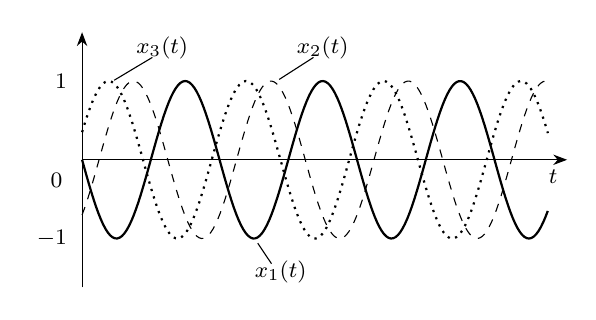
\begin{tikzpicture}[x=0.97cm,y=1cm,every node/.style={font=\footnotesize}]
  % 坐标轴
  \draw[-{Stealth[length=5pt]}] (0,0) -- (6.35,0) node[below left] {$t$};
  \draw[-{Stealth[length=5pt]}] (0,-1.62) -- (0,1.62);
  \node[left] at (-0.07,1.00) {$1$};
  \node[left] at (-0.07,-1.00) {$-1$};
  \node[left] at (-0.13,-0.26) {$0$};
  % 三条不同初相的余弦（周期 1.8）
  \draw[thick] plot[domain=0:6.10,samples=200] (\x,{cos(deg(3.49066*\x+1.57080))});        % x1(t) 实线
  \draw[dashed] plot[domain=0:6.10,samples=200] (\x,{cos(deg(3.49066*\x-2.34600))});        % x2(t) 虚线
  \draw[dotted,thick] plot[domain=0:6.10,samples=220] (\x,{cos(deg(3.49066*\x-1.21300))});  % x3(t) 点线
  % 标注与引线
  \node at (1.05,1.42) {$x_3(t)$};
  \draw[thin] (0.92,1.30) -- (0.42,1.01);
  \node at (3.15,1.42) {$x_2(t)$};
  \draw[thin] (3.03,1.30) -- (2.58,1.02);
  \node at (2.60,-1.42) {$x_1(t)$};
  \draw[thin] (2.48,-1.32) -- (2.30,-1.06);
\end{tikzpicture}
\captionof{figure}{随相信号的样本函数}\label{fig:3.6}
\end{minipage}\hfill
\begin{minipage}[t]{0.43\linewidth}\centering
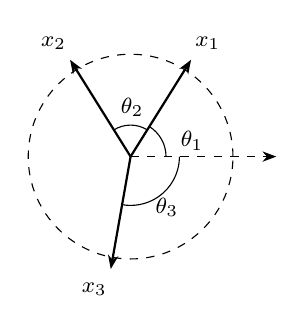
\begin{tikzpicture}[x=1cm,y=1cm,every node/.style={font=\footnotesize}]
  % 极坐标：虚线圆 + 水平参考方向
  \draw[dashed] (0,0) circle (1.30);
  \draw[dashed,-{Stealth[length=5pt]}] (0,0) -- (1.85,0);
  % 三个样本函数的相位箭头
  \draw[-{Stealth[length=5pt]},thick] (0,0) -- (58:1.45);
  \draw[-{Stealth[length=5pt]},thick] (0,0) -- (122:1.45);
  \draw[-{Stealth[length=5pt]},thick] (0,0) -- (260:1.45);
  % 相位角圆弧
  \draw[thin] (0.45,0) arc[start angle=0,end angle=58,radius=0.45];
  \draw[thin] (58:0.40) arc[start angle=58,end angle=122,radius=0.40];
  \draw[thin] (0.62,0) arc[start angle=0,end angle=-100,radius=0.62];
  % 角度与箭头标注
  \node at (0.78,0.20) {$\theta_1$};
  \node at (0.02,0.62) {$\theta_2$};
  \node at (0.46,-0.64) {$\theta_3$};
  \node at (0.98,1.44) {$x_1$};
  \node at (-0.98,1.44) {$x_2$};
  \node at (-0.46,-1.68) {$x_3$};
\end{tikzpicture}
\captionof{figure}{相位的不确定性}\label{fig:3.7}
\end{minipage}
\end{center}

图 3.7 用极坐标形式示意了其样本函数的相位情况\nobreak。由图可见\nobreak，随机谱函数均匀地取各种角度\nobreak，易见\nobreak，它的统计平均为零\nobreak，因而无法有效地描述 $X(t)$ 的频谱特性\nobreak。另一方面\nobreak，$X(t)$ 的功率谱为其相关函数的傅里叶变换\nobreak，即
% EQNUMBERS: 3.12, 3.13, 3.14, 3.15, 3.16, 3.17, 3.18, 3.19
% FIGNUMBERS: 3.4, 3.5, 3.6, 3.7
% PAGES: 72-74
% =====================================================================
%  frag_E —— 书 p.75–77（PDF p.89–91）
%  内容：§3.4.2 续（性质 1 功率谱密度的基本性质）、例3.9、单边功率谱、
%        图3.8、2. 互功率谱密度（定义3.8 = 式(3.23)、性质 2）、例3.10、
%        §3.4.3* 维纳-辛钦定理的证明（①②、截断信号、定理与完整证明）、
%        图3.9、图3.10、式(3.24)(3.25)
%  本片编号公式：(3.20)–(3.25)；图3.8、图3.9、图3.10（(a)(b) 两子图）
%  灰底框：例3.9（p.75 约 0.35–0.55）、例3.10（p.76 约 0.33–0.72），
%          两个框都在本片内开、本片内闭，不跨页。
%  接缝：D→E 是 tight_seam —— 本片首行是 frag_D 末句"…即"之后的**无编号**公式，
%        故本片**不写"即"**，装配时由 retypeset.py 用单个换行接成同一句。
%        本片正常收尾（p.77 页末图3.10 图注），frag_F 从 §3.5 起笔。
% =====================================================================
\[
R(\tau)=\frac{1}{2}\cos(\omega_0\tau)\longleftrightarrow S(\omega)=\frac{\pi}{2}\left[\delta(\omega-\omega_0)+\delta(\omega+\omega_0)\right]
\]
虽然损失了相位特性\nobreak，但功率谱仍能有效地刻画出 $X(t)$ 的信号成分在频域上的分布状况\nobreak。

可见\nobreak，平稳随机信号的功率谱密度是一个确定的谱函数\nobreak；而信号本身的傅里叶变换是随机的谱函数\nobreak。显然\nobreak，通过功率谱可以更为明确地说明随机信号中各频率成分的含量\nobreak。因此\nobreak，与确定信号不同的是\nobreak，随机信号的频域分析主要是考察它的功率谱\nobreak，而非信号谱\nobreak。

\thm{性质 1}（功率谱密度的基本性质\nobreak）平稳信号的功率谱总是正的实偶函数\nobreak，即 $S_X(-\omega)=S_X(\omega)\geqslant 0$\nobreak。

\textbf{证明\nobreak：}由于 $R_X(\tau)$ 是实偶函数\nobreak，由傅里叶变换的性质\nobreak，$S_X(\omega)$ 也一定是实偶函数\nobreak。还可以证明\nobreak：$S_X(\omega)$ 总是正数\nobreak，这符合功率的物理意义\nobreak。

% 原书如此（疑似笔误）：印的是 $1-\eu^{-(\omega-1)^2}$，而该式恒为非负，
% 与下文"可能为负"矛盾；疑应为 $1-\eu^{(\omega-1)^2}$。按保真纪律原样保留。
利用上面的性质\nobreak，可以判别功率谱表达式的正确性\nobreak。例如\nobreak，$\dfrac{\omega^2}{\omega^4+\ju2\omega^2+1}$ 可能为虚数\nobreak；$1-\eu^{-(\omega-1)^2}$ 可能为负\nobreak，而且它也不是偶函数\nobreak。因此\nobreak，它们都不是正确的功率谱表达式\nobreak。

\begin{examplebox}
\textbf{例3.9}\quad 已知随机信号 $X(t)$ 的功率谱 $S(\omega)=\dfrac{\omega^2+4}{\omega^4+10\omega^2+9}$\nobreak，求其自相关函数与均方值\nobreak。

\textbf{解\nobreak：}\quad 首先进行分解\nobreak，有
\[
S(\omega)=\frac{\omega^2+4}{\omega^4+10\omega^2+9}=\frac{\omega^2+4}{(\omega^2+9)(\omega^2+1)}=\frac{5/8}{\omega^2+9}+\frac{3/8}{\omega^2+1}
\]
利用傅里叶变换公式\nobreak：$\eu^{-a\lvert t\rvert}\longleftrightarrow 2a/(\omega^2+a^2)$\nobreak，其中 $a>0$\nobreak，可以求得
\[
R(\tau)=\frac{5}{48}\eu^{-3\lvert\tau\rvert}+\frac{3}{16}\eu^{-\lvert\tau\rvert}
\]
进而\nobreak，均方值 $R(0)=7/24$\nobreak。
\end{examplebox}

由相关函数的实偶特性与功率谱的正实偶特性不难发现在常用的傅里叶变换对关系中\nobreak，只有部分适合于 $R_X(\tau)$ 与 $S_X(\omega)$ 对\nobreak。

由于 $R_X(\tau)$ 与 $S_X(\omega)$ 都是实偶函数\nobreak，这种情况下\nobreak，只需关心 $\eu^{\ju\omega\tau}$ 的实部\nobreak，于是可得
\begin{equation}
S_X(\omega)=\int_{-\infty}^{+\infty}R_X(\tau)\cos\omega\tau\dif\tau=2\int_{0}^{+\infty}R_X(\tau)\cos\omega\tau\dif\tau
\label{eq:3.20}
\end{equation}
\begin{equation}
R_X(\tau)=\frac{1}{2\pi}\int_{-\infty}^{+\infty}S_X(\omega)\cos\omega\tau\dif\omega=\frac{1}{\pi}\int_{0}^{+\infty}S_X(\omega)\cos\omega\tau\dif\omega
\label{eq:3.21}
\end{equation}
鉴于实信号的功率谱固有的偶函数特点\nobreak，应用中经常只使用正频率部分\nobreak，称它为单边功率谱\nobreak。相对地\nobreak，有时称原定义为双边功率谱\nobreak。其实\nobreak，频率的基本物理意义是单位时间内某物理量的反复次数\nobreak，而负频率只有纯粹数学上的意义与分析上的方便\nobreak。显然\nobreak，在实际应用中使用单边功率谱有着更直观的物理意义\nobreak，因此\nobreak，它有时也被称为物理功率谱\nobreak。

如果记单边功率谱为 $G_X(\omega)$\nobreak，为了保持计算出的功率一样\nobreak，有
\begin{equation}
G_X(\omega)=\begin{cases}2S_X(\omega), & \omega>0\\ 0, & \omega<0\end{cases}
\label{eq:3.22}
\end{equation}
如图 3.8 所示\nobreak。

\begin{figure}[htbp]
\centering
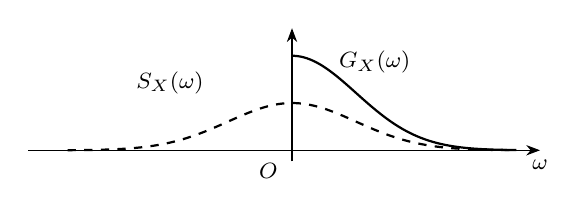
\begin{tikzpicture}[x=1cm,y=1cm,every node/.style={font=\footnotesize}]
  % ω 轴（横轴）与纵轴
  \draw[-{Stealth[length=5pt]}] (-3.35,0) -- (3.15,0) node[below] {$\omega$};
  \draw[-{Stealth[length=5pt]}] (0,-0.14) -- (0,1.55);
  \node[below left] at (-0.06,-0.04) {$O$};
  % S_X(ω)：双边（虚线、偶函数）
  \draw[dashed,thick] plot[domain=-2.85:2.85,samples=120] (\x,{0.60*exp(-(\x/1.15)*(\x/1.15))});
  % G_X(ω)：单边（实线，ω>0，恒为 S_X 的 2 倍）
  \draw[thick] plot[domain=0:2.85,samples=90] (\x,{1.20*exp(-(\x/1.15)*(\x/1.15))});
  \node at (-1.55,0.86) {$S_X(\omega)$};
  \node at (1.05,1.12) {$G_X(\omega)$};
\end{tikzpicture}
\caption{单边与双边功率谱}\label{fig:3.8}
\end{figure}

\bhead{2.\ 互功率谱密度}

\thm{定义 3.8} 联合平稳信号 $X(t)$ 与 $Y(t)$ 的互功率谱密度定义为其互相关函数 $R_{XY}(\tau)$ 与 $R_{YX}(\tau)$ 的傅里叶变换\nobreak，即
\begin{equation}
S_{XY}(\omega)=\int_{-\infty}^{+\infty}R_{XY}(\tau)\eu^{-\ju\omega\tau}\dif\tau,\quad
S_{YX}(\omega)=\int_{-\infty}^{+\infty}R_{YX}(\tau)\eu^{-\ju\omega\tau}\dif\tau
\label{eq:3.23}
\end{equation}
它们简称为互功率谱\fw{Cross Power Spectral Density}\nobreak。

互功率谱常常是复函数\nobreak，它反映了两个信号的关联性沿 $\omega$ 轴的密度状况\nobreak。如果 $S_{XY}(\omega)$ 很大\nobreak，表明两个信号的相应频率分量关联度很高\nobreak；如果 $S_{XY}(\omega)=0$\nobreak，表明它们的相应频率分量是正交的\nobreak。根据定义还容易证明互功率谱的以下性质\nobreak：

% 原书如此：第二式两端都印作 $S_{XY}$（$S_{XY}^{*}(\omega)=S_{XY}(-\omega)$），
% 已 6 倍放大逐字核对；数学上成立（实 $R_{XY}$），但左端易被误读为 $S_{YX}$。
\thm{性质 2}（互功率谱具有对称性\nobreak）$S_{XY}^{*}(\omega)=S_{YX}(\omega)$\nobreak；$S_{XY}^{*}(\omega)=S_{XY}(-\omega)$

可见\nobreak，两种互功率谱的实部相同\nobreak，而虚部反号\nobreak；实信号的互相关函数为实函数\nobreak，因此\nobreak，互功率谱的实部都是偶函数\nobreak，虚部都是奇函数\nobreak。

\begin{examplebox}
\textbf{例3.10}\quad 讨论（加性\nobreak）单频干扰\nobreak。若实平稳随机信号 $X(t)$ 受到加性的独立随机正弦分量 $Z(t)=A\cos(\omega_0t+\Theta)$ 的干扰\nobreak。已知 $A,\omega_0$ 为常数\nobreak，$\Theta$ 是在 $[0,2\pi)$ 上均匀分布的随机变量\nobreak。试求\nobreak：

\fw{1}受扰后的信号 $Y(t)=X(t)+Z(t)$ 的相关函数 $R_Y(t+\tau,t)$\nobreak；

\fw{2}信号 $X(t)$ 与 $Y(t)$ 是否联合平稳\nobreak？如果是\nobreak，进一步求解功率谱 $S_Y(\omega)$ 与互功率谱 $S_{XY}(\omega)$\nobreak。

\textbf{解\nobreak：}\quad\fw{1}\quad $\E[Z(t)]=A\E[\cos(\omega_0t+\Theta)]=0$
\[
R_Z(t+\tau,t)=\E\left[A\cos(\omega_0t+\omega_0\tau+\Theta)A\cos(\omega_0t+\Theta)\right]=\frac{1}{2}A^2\cos\omega_0\tau
\]
由于 $X(t)$ 与 $Z(t)$ 独立\nobreak，且 $Z(t)$ 是零均值的\nobreak，因此它们正交\nobreak。对于 $Y(t)=X(t)+Z(t)$\nobreak，有
\[
\begin{aligned}
R_Y(t+\tau,t)&=\E\left\{[X(t+\tau)+Z(t+\tau)][X(t)+Z(t)]\right\}\\
&=R_X(t+\tau,t)+R_Z(t+\tau,t)=R_X(\tau)+\frac{1}{2}A^2\cos\omega_0\tau
\end{aligned}
\]
$X(t)$ 与 $Z(t)$ 的正交性使得上式推导中的交叉项为零\nobreak。

\fw{2}因此\nobreak，$Y(t)$ 是平稳信号\nobreak。仿上有
\[
R_{XY}(t+\tau,t)=\E\left\{X(t+\tau)[X(t)+Z(t)]\right\}=R_X(\tau)
\]
因此\nobreak，$X(t)$ 与 $Y(t)$ 是联合平稳的\nobreak。通过傅里叶变换可得
\[
S_Y(\omega)=S_X(\omega)+\frac{\pi A^2}{2}\left[\delta(\omega-\omega_0)+\delta(\omega+\omega_0)\right]
\]
\[
S_{XY}(\omega)=S_X(\omega)
\]
另外\nobreak，从 $Y(t)$ 的相关函数与功率谱中可以看到其中包含的周期分量\nobreak，即单频干扰成分 $\omega_0$\nobreak。
\end{examplebox}

\ssubsection{维纳-辛钦定理的证明}
下面首先详细说明确定信号的能量谱密度与功率谱密度\nobreak。

\begin{citemize}
\item ① 对能量型信号\nobreak，定义能量谱密度为 $\left|X(\ju\omega)\right|^2$\nobreak，其中 $X(\ju\omega)$ 为 $x(t)$ 的傅里叶变换\nobreak。利用巴塞伐尔公式可发现\nobreak，其基本物理意义反映在下式中
\[
E=\int_{-\infty}^{+\infty}x^2(t)\dif t=\frac{1}{2\pi}\int_{-\infty}^{+\infty}\left|X(\ju\omega)\right|^2\dif\omega
\]
\item ② 对于功率型信号\nobreak，定义功率谱密度为
\[
S(\omega)=\lim_{T\to\infty}\frac{1}{2T}\left|X_T(\ju\omega)\right|^2
\]
\end{citemize}

% 原书 p.77 首行"式中，…"顶格（是 ② 条正文的续行，无首行缩进），故加 \noindent
\noindent 式中\nobreak，$X_T(\ju\omega)$ 是 $x_T(t)$ 的傅里叶变换\nobreak，而 $x_T(t)$ 称为截断信号\nobreak，它是从 $x(t)$ 上截取的 $[-T,+T]$ 段\nobreak，它在 $[-T,+T]$ 区间以外为零\nobreak，如图 3.9 所示\nobreak。

\begin{figure}[htbp]
\centering
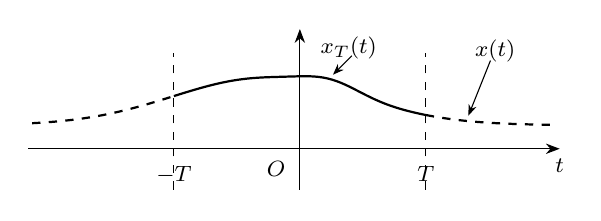
\begin{tikzpicture}[x=1cm,y=1cm,every node/.style={font=\footnotesize}]
  % t 轴与纵轴
  \draw[-{Stealth[length=5pt]}] (-3.45,0) -- (3.30,0) node[below] {$t$};
  \draw[-{Stealth[length=5pt]}] (0,-0.52) -- (0,1.52);
  \node[below left] at (-0.06,-0.04) {$O$};
  % ±T 处的虚线
  \draw[dashed] (-1.60,-0.52) -- (-1.60,1.22);
  \draw[dashed] (1.60,-0.52) -- (1.60,1.22);
  \node[below] at (-1.60,-0.10) {$-T$};
  \node[below] at (1.60,-0.10) {$T$};
  % x(t)：[-T,T] 以外（虚线）
  \draw[dashed,thick] plot[domain=-3.40:-1.60,samples=40] (\x,{0.30+0.60*exp(-((\x+0.45)/1.65)*((\x+0.45)/1.65))+0.12*exp(-((\x-0.40)/0.50)*((\x-0.40)/0.50))});
  \draw[dashed,thick] plot[domain=1.60:3.25,samples=40] (\x,{0.30+0.60*exp(-((\x+0.45)/1.65)*((\x+0.45)/1.65))+0.12*exp(-((\x-0.40)/0.50)*((\x-0.40)/0.50))});
  % x_T(t)：[-T,T] 以内（实线）
  \draw[thick] plot[domain=-1.60:1.60,samples=60] (\x,{0.30+0.60*exp(-((\x+0.45)/1.65)*((\x+0.45)/1.65))+0.12*exp(-((\x-0.40)/0.50)*((\x-0.40)/0.50))});
  % 标注与引线
  \node at (0.62,1.28) {$x_T(t)$};
  \draw[-{Stealth[length=4pt]}] (0.66,1.18) -- (0.42,0.94);
  \node at (2.48,1.24) {$x(t)$};
  \draw[-{Stealth[length=4pt]}] (2.42,1.12) -- (2.14,0.42);
\end{tikzpicture}
\caption{截断信号图示}\label{fig:3.9}
\end{figure}

相仿地\nobreak，其基本物理意义反映在下式中
\[
\begin{aligned}
P&=\lim_{T\to\infty}\frac{1}{2T}\int_{-T}^{T}x^2(t)\dif t=\lim_{T\to\infty}\frac{1}{2T}\left[\int_{-\infty}^{+\infty}x_T^2(t)\dif t\right]\\
&=\lim_{T\to\infty}\frac{1}{2T}\left[\frac{1}{2\pi}\int_{-\infty}^{+\infty}\left|X_T(\ju\omega)\right|^2\dif\omega\right]\\
&=\frac{1}{2\pi}\int_{-\infty}^{+\infty}\left[\lim_{T\to\infty}\frac{1}{2T}\left|X_T(\ju\omega)\right|^2\right]\dif\omega=\frac{1}{2\pi}\int_{-\infty}^{+\infty}S(\omega)\dif\omega
\end{aligned}
\]
可见\nobreak，信号的能量谱密度或功率谱密度沿整个频率轴上的积分正好是信号的能量或功率\nobreak。

对于随机信号 $X(t)$\nobreak，记其样本函数为 $X(t,\xi)$\nobreak，则样本功率谱定义为
\begin{equation}
S_s(\omega,\xi)=\lim_{T\to\infty}\frac{1}{2T}\left|X_T(\ju\omega,\xi)\right|^2
\label{eq:3.24}
\end{equation}
随机信号的功率谱密度定义为
\begin{equation}
S(\omega)=\E\left[S_s(\omega)\right]=\lim_{T\to\infty}\frac{1}{2T}\E\left[\left|X_T(\ju\omega)\right|^2\right]
\label{eq:3.25}
\end{equation}

\thm{维纳-辛钦定理} 平稳随机信号的功率谱密度满足\nobreak：$R(\tau)\longleftrightarrow S(\omega)$\nobreak。

\textbf{证明\nobreak：}
\[
X_T(\ju\omega,\xi)=\int_{-\infty}^{+\infty}X_T(t,\xi)\eu^{-\ju\omega t}\dif t=\int_{-T}^{T}X(t,\xi)\eu^{-\ju\omega t}\dif t
\]
因此
\[
\begin{aligned}
\left|X_T(\ju\omega,\xi)\right|^2&=\left[\int_{-T}^{T}X(u,\xi)\eu^{-\ju\omega u}\dif u\right]\left[\int_{-T}^{T}X(v,\xi)\eu^{-\ju\omega v}\dif v\right]^{*}\\
&=\int_{-T}^{T}\int_{-T}^{T}X(u,\xi)X^{*}(v,\xi)\eu^{-\ju\omega(u-v)}\dif u\dif v
\end{aligned}
\]
进而
\[
S(\omega)=\lim_{T\to\infty}\frac{1}{2T}\E\left[\left|X_T(\ju\omega,\xi)\right|^2\right]=\lim_{T\to\infty}\frac{1}{2T}\int_{-T}^{T}\int_{-T}^{T}R(u-v)\eu^{-\ju\omega(u-v)}\dif u\dif v
\]
作变换 $\begin{cases}t=v\\ \tau=u-v\end{cases}$\nobreak，$\begin{cases}v=t\\ u=t+\tau\end{cases}$\nobreak，于是 $\lvert\bm{J}\rvert=\begin{vmatrix}1&0\\1&1\end{vmatrix}=1$\nobreak。积分区域的变化如图 3.10 所示\nobreak，因此
% 原书该式四行排满版心；本文正文字号比原书大，按第1章式(1.17) 的先例
% 用 \resizebox 等比压到版心内（仍是矢量文字），四行结构与原书一致
\[
\resizebox{\linewidth}{!}{$\displaystyle
\begin{aligned}
S(\omega)&=\lim_{T\to\infty}\frac{1}{2T}\left\{\int_{-2T}^{0}\left[\int_{-T-\tau}^{T}R(\tau)\eu^{-\ju\omega\tau}\dif t\right]\dif\tau+\int_{0}^{2T}\left[\int_{-T}^{T-\tau}R(\tau)\eu^{-\ju\omega\tau}\dif t\right]\dif\tau\right\}\\
&=\lim_{T\to\infty}\frac{1}{2T}\left\{\int_{-2T}^{0}(2T+\tau)R(\tau)\eu^{-\ju\omega\tau}\dif\tau+\int_{0}^{2T}(2T-\tau)R(\tau)\eu^{-\ju\omega\tau}\dif\tau\right\}\\
&=\lim_{T\to\infty}\int_{-2T}^{2T}\left(1-\frac{\lvert\tau\rvert}{2T}\right)R(\tau)\eu^{-\ju\omega\tau}\dif\tau\\
&=\int_{-\infty}^{+\infty}R(\tau)\eu^{-\ju\omega\tau}\dif\tau
\end{aligned}$}
\]
即 $R(\tau)\longleftrightarrow S(\omega)$\nobreak。

\begin{figure}[htbp]
\centering
\begin{minipage}[t]{0.40\linewidth}\centering
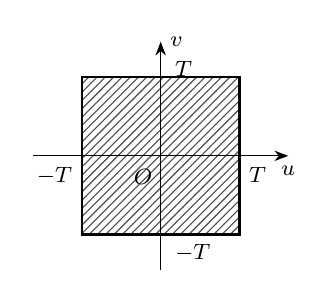
\begin{tikzpicture}[x=1cm,y=1cm,scale=1.00,every node/.style={font=\footnotesize}]
  % 积分区域：u、v 平面上的正方形 [-T,T]×[-T,T]
  \fill[pattern=north east lines,pattern color=black!70] (-1,-1) rectangle (1,1);
  \draw[thick] (-1,-1) rectangle (1,1);
  % 坐标轴
  \draw[-{Stealth[length=5pt]}] (-1.62,0) -- (1.62,0) node[below] {$u$};
  \draw[-{Stealth[length=5pt]}] (0,-1.45) -- (0,1.45) node[right] {$v$};
  \node[below left] at (0.02,-0.05) {$O$};
  \node[below left] at (-1.0,-0.02) {$-T$};
  \node[below right] at (1.0,-0.02) {$T$};
  \node[right] at (0.06,1.10) {$T$};
  \node[below right] at (0.06,-1.0) {$-T$};
\end{tikzpicture}
\par\smallskip
\end{minipage}\hfill
\begin{minipage}[t]{0.56\linewidth}\centering
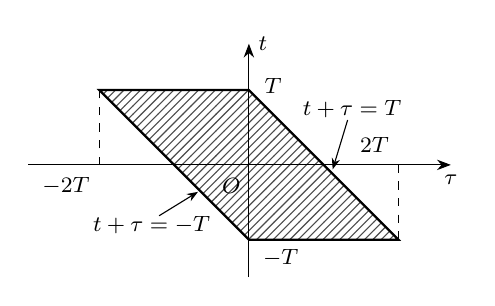
\begin{tikzpicture}[x=1cm,y=1cm,scale=0.95,every node/.style={font=\footnotesize}]
  % 积分区域：τ、t 平面上的平行四边形 (-2T,T)→(0,T)→(2T,-T)→(0,-T)
  \fill[pattern=north east lines,pattern color=black!70] (-2,1) -- (0,1) -- (2,-1) -- (0,-1) -- cycle;
  \draw[thick] (-2,1) -- (0,1) -- (2,-1) -- (0,-1) -- cycle;
  % 坐标轴
  \draw[-{Stealth[length=5pt]}] (-2.95,0) -- (2.70,0) node[below] {$\tau$};
  \draw[-{Stealth[length=5pt]}] (0,-1.50) -- (0,1.62) node[right] {$t$};
  \node[below left] at (0.02,-0.05) {$O$};
  % ±2T 处的虚线
  \draw[dashed] (-2.0,0) -- (-2.0,1.0);
  \draw[dashed] (2.0,0) -- (2.0,-1.0);
  \node[below left] at (-2.0,-0.04) {$-2T$};
  \node[above left] at (2.0,0.04) {$2T$};
  \node[right] at (0.08,1.06) {$T$};
  \node[below right] at (0.06,-1.0) {$-T$};
  % 两条斜边的标注与引线
  \node at (1.38,0.74) {$t+\tau=T$};
  \draw[-{Stealth[length=4pt]}] (1.32,0.60) -- (1.12,-0.06);
  \node at (-1.30,-0.80) {$t+\tau=-T$};
  \draw[-{Stealth[length=4pt]}] (-1.20,-0.68) -- (-0.68,-0.36);
\end{tikzpicture}
\par\smallskip
\end{minipage}
\caption{积分区域的变化}\label{fig:3.10}
\end{figure}

% EQNUMBERS: 3.20, 3.21, 3.22, 3.23, 3.24, 3.25
% FIGNUMBERS: 3.8, 3.9, 3.10
% PAGES: 75-77

% =====================================================================
%  frag_F —— 书 p.78–80（PDF p.92–94）
%  内容：3.5 白噪声与热噪声、3.5.1 白噪声、定义3.9、(3.26)(3.27)、图3.11、
%        高斯白噪声、白噪声序列、例3.11、3.5.2* 热噪声、图3.12、
%        (3.28)(3.29)(3.30)(3.31)、3.6 应用举例、例3.12、例3.13、例3.14 题面
%  本片编号公式：(3.26)–(3.32)；图3.11、图3.12（图3.12 原书右侧绕排，本重排改居中）
%  灰底框：例3.11（p.79，页内闭合）；例3.12（p.80，页内闭合）；
%          例3.13 + 例3.14 是**同一个框**，p.80 起 → 延续到 frag_G，
%          本片**有意不写 \end{examplebox}**（由 frag_G 在 p.82 图3.16 之后闭合）
%  接缝 F→G：本片停在「…$X(t)$」半句上，frag_G 从「为实广义平稳随机信号…」续写
% =====================================================================

\section{白噪声与热噪声}
考虑一种理想与简单的随机信号\nobreak，其功率谱为常数\nobreak，这就引出了白噪声的概念\nobreak，它具有重要的理论价值\nobreak。工程实践中的一些信号在特定的条件下可以近似为这种信号\nobreak，例如\nobreak，（电阻\nobreak）热噪声\nobreak。

\subsection{白噪声}
\thm{定义 3.9} 若广义平稳信号 $\{X(t),t\in T\}$ 对任意 $t+\tau,t\in T$\nobreak，恒有
\begin{equation}
R(\tau)=\frac{N_0}{2}\delta(\tau),\quad S(\omega)=\frac{N_0}{2}
\label{eq:3.26}
\end{equation}
则称它是（平稳\nobreak）白噪声信号\fw{White Noise Signal}\nobreak，简称白噪声或白信号\nobreak。

通常假定白噪声总是零均值的\nobreak，因此\nobreak，$C(\tau)=R(\tau)$\nobreak。白噪声是一种具有无限带宽的理想随机信号\nobreak，如图~\ref{fig:3.11}(a)所示\nobreak。由于功率谱为常数\nobreak，具有与光学中白色光类似的功率分布性质\nobreak，因此它被称为白色的\nobreak。相对地\nobreak，我们定义任意非白色噪声为\textbf{有色噪声}\fw{Colored Noise}\nobreak，简称色噪声\nobreak，如图~\ref{fig:3.11}(b)所示\nobreak。白噪声定义中采用常数 $N_0/2$\nobreak，而它的单边功率谱值正好是 $N_0$\nobreak，后面会看到这样取值便于分析与计算\nobreak。由定义可知\nobreak，白噪声信号的功率（即方差\nobreak）为无穷大\nobreak，而不同时刻上的随机变量彼此不相关\nobreak，有时也通俗地称这种信号是“纯随机的”\nobreak。容易知道\nobreak，白噪声的相关系数为
\begin{equation}
\rho(\tau)=\frac{C(\tau)}{C(0)}=\frac{R(\tau)}{R(0)}=\begin{cases}1, & \tau=0\\ 0, & \tau\neq0\end{cases}
\label{eq:3.27}
\end{equation}

\begin{figure}[htbp]
\centering
\begin{tikzpicture}[x=1cm,y=1cm,every node/.style={font=\footnotesize}]
  % ---------- (a) 白噪声：左 R_N(τ)，右 S_N(ω) ----------
  \draw[-{Stealth[length=4pt]}] (-0.75,0) -- (1.95,0) node[below] {$\tau$};
  \draw[-{Stealth[length=4pt]}] (0,-0.40) -- (0,1.95) node[right] {$R_N(\tau)$};
  % δ 冲激：origin 处的竖直箭头，高度 N_0/2
  \draw[very thick,-{Stealth[length=6pt]}] (0,0) -- (0,1.15);
  \node[right] at (0.06,0.62) {$N_0/2$};
  \node[below left] at (0.02,-0.02) {$O$};
  % 傅里叶变换对：双向箭头
  \draw[{Stealth[length=4pt]}-{Stealth[length=4pt]}] (2.30,0.95) -- (3.10,0.95);
  % S_N(ω)：常数谱
  \draw[-{Stealth[length=4pt]}] (3.30,0) -- (5.75,0) node[below] {$\omega$};
  \draw[-{Stealth[length=4pt]}] (3.95,-0.40) -- (3.95,1.95) node[right] {$S_N(\omega)$};
  \draw[thick] (3.40,1.15) -- (5.45,1.15);
  \node[above right] at (3.97,1.15) {$N_0/2$};
  \node[below left] at (3.97,-0.02) {$O$};
  \node at (2.45,-1.05) {(a) 白噪声};
  % ---------- (b) 色噪声：S_X(ω) 钟形 ----------
  \draw[-{Stealth[length=4pt]}] (7.45,0) -- (8.95,0) node[below] {$\omega$};
  \draw[-{Stealth[length=4pt]}] (8.15,-0.40) -- (8.15,1.95) node[right] {$S_X(\omega)$};
  \draw[thick,domain=7.55:8.75,samples=80] plot (\x,{1.15*exp(-((\x-8.15)^2)/(2*0.23*0.23))});
  \node[below left] at (8.17,-0.02) {$O$};
  \node at (8.15,-1.05) {(b) 色噪声};
\end{tikzpicture}
\caption{白噪声与色噪声}\label{fig:3.11}
\end{figure}

若白噪声的每个随机变量都服从高斯分布\nobreak，则称它为高斯白噪声（信号\nobreak）\fw{WGN, White Gaussian Noise}\nobreak。根据高斯信号的性质容易知道\nobreak，它是无关信号\nobreak，也就是独立信号\nobreak。可见\nobreak，高斯白噪声是极其理想的\nobreak，它代表着信号“随机性”的一种极限\nobreak。尽管知道了该信号的概率特性\nobreak，但由于其方差为无穷大\nobreak，我们无法写出其概率分布函数或密度函数\nobreak。

相仿地\nobreak，如果平稳序列对所有 $m$\nobreak，恒有相关函数 $R[m]=\dfrac{N_0}{2}\delta[m]$\nobreak，功率谱（参见 5.5 节\nobreak）$S(\eu^{\ju\omega})=N_0/2$\nobreak，则称它是白噪声序列\nobreak。注意\nobreak，与连续信号不同\nobreak，离散冲激函数 $\delta[m]$ 在 $m=0$ 是有限的\nobreak，因此\nobreak，白噪声序列的方差（或功率\nobreak）是有限的\nobreak，取值 $N_0/2$\nobreak。另外\nobreak，高斯白噪声序列也是独立序列\nobreak，其独立性使我们很容易写出它的任意阶概率密度函数\nobreak。

\begin{examplebox}
\textbf{例3.11}\quad 若 $N(n)$ 是方差为 $\sigma^2$ 的零均值高斯白序列\nobreak，试求\nobreak：

\fw{1}它的相关函数 $R[n_1,n_2]$ 与协方差函数 $C[n_1,n_2]$\nobreak；\fw{2}它的 $n$ 维概率密度函数\nobreak。

\textbf{解\nobreak：}\quad $R[n_1,n_2]=C[n_1,n_2]=\sigma^2\delta[n_1-n_2]$

作为高斯白噪声\nobreak，$N(n)$ 也是同分布的独立信号\nobreak，于是可得
% 原书该式单行排满版心；本文正文字号比原书大，天然宽度超版心（13pt），
% 按第1章 式(1.17) 的先例用 \resizebox 等比压到版心内（仍是矢量文字）
\[
\resizebox{\linewidth}{!}{$\displaystyle
f(x_1,x_2,\cdots,x_n;n_1,n_2,\cdots,n_n)=\prod_{i=1}^{n}f(x_i)=\frac{1}{(2\pi)^{n/2}\sigma^n}\exp\left(-\frac{1}{2\sigma^2}\sum_{i=1}^{n}x_i^2\right)$}
\]
\end{examplebox}

% 3.5.2* 是带星号的选学小节：原书星号紧跟在编号后面（3.5.2*　热噪声）。
% 用导言区的 \ssubsection：本次调用的作用域内给 \thesubsection 补星号，
% 自动编号（3.5.2*）与目录项都由它生成，作用域外复原。
\ssubsection{热噪声}
工程上的电阻热噪声\fw{Thermal Noise}很接近于理想的白噪声\nobreak。当温度高于绝对零度时\nobreak，实际电阻器中的自由电子呈现出随机骚动\nobreak，在电阻的两端形成噪声电压\nobreak。阻值为 $R$ 的有噪电阻器可表征为如图~\ref{fig:3.12} 所示的两种等效电路\nobreak。其中 $R$ 为理想的无噪电阻\nobreak，$V_n(t)$ 与 $I_n(t)$ 为随机的噪声电压源与电流源\nobreak。

\begin{figure}[htbp]
\centering
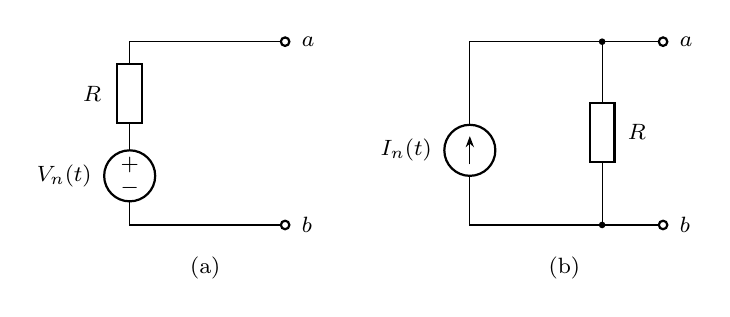
\begin{tikzpicture}[x=1.2cm,y=1.2cm,every node/.style={font=\footnotesize}]
  % ---------- (a) 电压源形式 ----------
  \draw (0,1.86) -- (0,2.10) -- (1.60,2.10);
  \draw[thick] (-0.13,1.24) rectangle (0.13,1.86);
  \node[left] at (-0.20,1.55) {$R$};
  \draw (0,1.24) -- (0,0.95);
  \draw[thick] (0,0.68) circle (0.27);
  \node at (0,0.79) {$+$};
  \node at (0,0.55) {$-$};
  \node[left] at (-0.30,0.68) {$V_n(t)$};
  \draw (0,0.41) -- (0,0.16) -- (1.60,0.16);
  \draw[thick] (1.645,2.10) circle (0.045);
  \node[right] at (1.72,2.10) {$a$};
  \draw[thick] (1.645,0.16) circle (0.045);
  \node[right] at (1.72,0.16) {$b$};
  \node at (0.80,-0.30) {(a)};
  % ---------- (b) 电流源形式 ----------
  \draw (3.60,1.22) -- (3.60,2.10) -- (5.60,2.10);
  \draw (3.60,0.68) -- (3.60,0.16) -- (5.60,0.16);
  \draw[thick] (3.60,0.95) circle (0.27);
  \draw[-{Stealth[length=4pt]}] (3.60,0.80) -- (3.60,1.10);
  \node[left] at (3.30,0.95) {$I_n(t)$};
  \draw (5.00,2.10) -- (5.00,1.45);
  \draw (5.00,0.83) -- (5.00,0.16);
  \draw[thick] (4.87,0.83) rectangle (5.13,1.45);
  \node[right] at (5.17,1.14) {$R$};
  \fill (5.00,2.10) circle (0.035);
  \fill (5.00,0.16) circle (0.035);
  \draw[thick] (5.645,2.10) circle (0.045);
  \node[right] at (5.72,2.10) {$a$};
  \draw[thick] (5.645,0.16) circle (0.045);
  \node[right] at (5.72,0.16) {$b$};
  \node at (4.60,-0.30) {(b)};
\end{tikzpicture}
\caption{有噪声电阻器的等效电路}\label{fig:3.12}
\end{figure}

考虑电压源的等效形式\nobreak，物理学家通过大量的实验与理论分析发现\nobreak，随机电压源 $V_n(t)$ 是零均值的\nobreak，它的单边功率谱可以表示为
\begin{equation}
G_V(\omega)=\frac{2R}{\pi}\left(\frac{\omega h}{2}+\frac{\omega h}{\eu^{\omega h/(2\pi kT)}-1}\right),\quad \omega\geqslant0
\label{eq:3.28}
\end{equation}
式中\nobreak，$h=6.63\times10^{-34}\ \mathrm{J}\cdot\mathrm{s}$（普朗克常数\nobreak）\nobreak，$k=1.38\times10^{-23}\ \mathrm{J}/\mathrm{K}$（玻耳兹曼常数\nobreak）\nobreak，$T=(273+C)\ \mathrm{K}$（绝对温度\nobreak）\nobreak，$C$ 为摄氏温度\nobreak。由于 $V_n(t)$ 的具体物理含义为电压（单位\nobreak：V\nobreak）\nobreak，因而\nobreak，$G_V(\omega)$ 的物理本质为单位带宽的均方电压（$\mathrm{V}^2/\mathrm{Hz}$\nobreak）\nobreak。

在常温下\nobreak，对于高达 1000 GHz 的频率\nobreak，$\omega h/(2\pi kT)<0.2$\nobreak，因此\nobreak，可利用近似公式 $\eu^{x}\approx1+x$ 得到
\begin{equation}
G_V(\omega)\approx4kTR\quad \mathrm{V}^2/\mathrm{Hz},\quad \omega\geqslant0
\label{eq:3.29}
\end{equation}
或者\nobreak，对于电流源形式\nobreak，可令电导 $G=1/R$\nobreak，则随机电流源 $I_n(t)$ 的单边功率谱为
\begin{equation}
G_I(\omega)\approx4kTG\quad \mathrm{A}^2/\mathrm{Hz},\quad \omega\geqslant0
\label{eq:3.30}
\end{equation}
1000 GHz 包含了几乎所有的实用频率\nobreak，因此\nobreak，电阻的热噪声被视为理想的白噪声信号\nobreak。

根据电路分析的知识\nobreak，当图~\ref{fig:3.12} 中的等效电路接上阻值为 $R$ 的负载时\nobreak，有噪电阻器将送出最大功率\nobreak，该最大值也称为电阻的可用（噪声\nobreak）功率\nobreak。由 $G_V(\omega)$ 的物理含义可知\nobreak，电阻器单位带宽的均方噪声电压为 $E(V_0^2)=4kTR$ $\mathrm{V}^2/\mathrm{Hz}$\nobreak。由于负载电阻上分到一半的噪声电压\nobreak，因此\nobreak，它在单位带宽上的可用（噪声\nobreak）功率为
\[
\frac{E(V_0^2)}{2^2}\div R=kT\quad \mathrm{W}/\mathrm{Hz}
\]
有时也称其为电阻热噪声的（单边\nobreak）可用功率谱\nobreak。注意\nobreak，它与电阻器的具体阻值无关\nobreak。

理论分析中时常使用双边功率谱形式\nobreak，则可令 $N_0=4kTR$\nobreak，于是\nobreak，阻值为 $R$ 的有噪电阻器的噪声电压信号的（双边\nobreak）功率谱为
\begin{equation}
S_V(\omega)=N_0/2=2kTR
\label{eq:3.31}
\end{equation}
电子热骚动的物理特性还使得这种噪声的统计特性具有平稳性并呈高斯分布\nobreak，因此分析中总是以平稳高斯白噪声作为其基本模型\nobreak，它的（双边\nobreak）功率谱为 $N_0/2=2kTR$（或 $N_0/2=2kTG$\nobreak）\nobreak。

% 3.6 起为 p.80 内容
\section{应用举例}
本节通过举例进一步说明随机信号平稳性的分析过程\nobreak，演示相关函数与功率谱的计算方法\nobreak；同时\nobreak，介绍随机二元传输信号与随机电报信号\nobreak，探讨它们的基本特性\nobreak。

\begin{examplebox}
\textbf{例3.12}\quad 若在 $27^{\circ}\mathrm{C}$ 使用带宽为 $B$Hz 的电压表测量 $R=1\ \mathrm{M}\Omega$ 电阻器两端的开路噪声电压\nobreak。求当带宽为 1 MHz 时\nobreak，理论上测得的有效（均方根\nobreak）电压值是多少\nobreak？

\textbf{解\nobreak：}\quad 任何实际的测量都只能获得一定带宽的信号成分\nobreak，本例中电压表测到的噪声电压部分只有 $B$Hz\nobreak，其均方值为 $E(V_0^2)=4kTRB$ $\mathrm{V}^2$\nobreak，因此\nobreak，测得的有效电压值为
% 该式超版心 28pt，按先例用 \resizebox 压到版心内
\[
\resizebox{\linewidth}{!}{$\displaystyle
V_{\mathrm{rms}}=\sqrt{4kTRB}=\sqrt{4\times1.38\times10^{-23}\times(273+27)\times10^6\times10^6}\approx1.29\times10^{-4}\ \mathrm{V}$}
\]
虽然 $V_{\mathrm{rms}}$ 只有 0.129 mV\nobreak，但当电路中具有高增益放大器时\nobreak，例如\nobreak，在高灵敏接收机的前端电路中\nobreak，这种噪声也是不可忽视的\nobreak。
\end{examplebox}

% 例3.13 + 例3.14 同处一个灰底框，本片只开框、不闭合（frag_G 在 p.82 图3.16 之后闭合）
\begin{examplebox}
\textbf{例3.13}\quad 讨论随机相位正弦信号的广义平稳条件\nobreak。

正弦随机信号 $X(t)=A\cos(\omega_0t+\Theta)$\nobreak，其中\nobreak，随机变量 $A$ 的均值为 $m_A$\nobreak，方差为 $\sigma_A^2$\nobreak，$\Theta$ 服从特征函数为 $\phi_{\Theta}(v)$ 的某种分布\nobreak，$\Theta$ 与 $A$ 统计独立\nobreak。讨论 $X(t)$ 的广义平稳性\nobreak。

\textbf{解\nobreak：}\quad 为了分析平稳性\nobreak，需要计算 $X(t)$ 的均值与自相关函数\nobreak。
\[
\E[X(t)]=m_A\E[\cos(\omega_0t+\Theta)]
\]
利用欧拉公式\nobreak：$\cos(\omega_0t+\Theta)=\dfrac{\eu^{\ju(\omega_0t+\Theta)}+\eu^{-\ju(\omega_0t+\Theta)}}{2}$\nobreak，有
% 该式（含编号）超版心 39pt，按先例用 \resizebox 压到版心内（编号仍在行右侧）
\begin{equation}
\resizebox{\dimexpr\linewidth-4em\relax}{!}{$\displaystyle
\E[X(t)]=\frac{m_A}{2}\left\{\E[\eu^{\ju(\omega_0t+\Theta)}]+\E[\eu^{-\ju(\omega_0t+\Theta)}]\right\}=\frac{m_A}{2}\left\{\eu^{\ju\omega_0t}\E[\eu^{\ju\Theta}]+\eu^{-\ju\omega_0t}\E[\eu^{-\ju\Theta}]\right\}$}
\label{eq:3.32}
\end{equation}
又根据特征函数的定义\nobreak，$\E[\eu^{\ju\Theta}]=\phi_{\Theta}(1)$\nobreak，$\E[\eu^{-\ju\Theta}]=\left\{\E[\eu^{\ju\Theta}]\right\}^{*}=\phi_{\Theta}^{*}(1)$\nobreak，因此\nobreak，当且仅当 $\phi_{\Theta}(1)=0$ 时\nobreak，$\E[X(t)]=0$（常数\nobreak）\nobreak。

\[
\begin{aligned}
\text{又}\qquad \E[X(t_1)X(t_2)]&=\E(A^2)\E[\cos(\omega_0t_1+\Theta)\cos(\omega_0t_2+\Theta)]\\
&=\frac{\E(A^2)}{2}\E[\cos\omega_0(t_1-t_2)+\cos(\omega_0t_1+\omega_0t_2+2\Theta)]
\end{aligned}
\]
对于上式中的第二项\nobreak，仿上利用欧拉公式\nobreak，并参照式\fw{3.32}的结果\nobreak，得到
\[
\E[\cos(\omega_0t_1+\omega_0t_2+2\Theta)]=\frac{1}{2}\left\{\eu^{\ju(\omega_0t_1+\omega_0t_2)}\E[\eu^{\ju2\Theta}]+\eu^{-\ju(\omega_0t_1+\omega_0t_2)}\E[\eu^{-\ju2\Theta}]\right\}
\]
因此\nobreak，当且仅当 $\phi_{\Theta}(2)=0$ 时\nobreak，上式为零\nobreak，使得
\[
\E[X(t_1)X(t_2)]=\frac{\E(A^2)}{2}\cos\omega_0(t_1-t_2)=\frac{\sigma_A^2+m_A^2}{2}\cos\omega_0(t_1-t_2)
\]
可见\nobreak，这类随机相位正弦信号广义平稳的充要条件是\nobreak：$\phi_{\Theta}(1)=\phi_{\Theta}(2)=0$\nobreak。此时
\[
\E[X(t)]=0,\quad R(t_1,t_2)=\frac{\E(A^2)}{2}\cos\omega_0(t_1-t_2)
\]
例如\nobreak，当 $\Theta$ 服从均匀分布 $U(-\pi,\pi)$ 时\nobreak，$\phi_{\Theta}(v)=\dfrac{\sin\pi v}{\pi v}$\nobreak，符合上述条件\nobreak，因而是广义平稳的\nobreak。

\textbf{例3.14}\quad 讨论乘法调制输出信号的功率谱\nobreak。

乘法调制输出信号 $Y(t)=X(t)\cos(\omega_0t+\Theta)$\nobreak，其中\nobreak，相位 $\Theta$ 服从均匀分布 $U(-\pi,\pi)$\nobreak，$X(t)$
% EQNUMBERS: 3.26, 3.27, 3.28, 3.29, 3.30, 3.31, 3.32
% FIGNUMBERS: 3.11, 3.12
% PAGES: 78-80
% NOTE: 本片末尾例3.13+例3.14 的灰底框**未闭合**，由 frag_G 收尾；F→G 为同段接缝。
% NOTE: 例3.11 的「解」后公式在原书中与「解：」同处一行（中间留宽空），此处按同一行转写。
% =====================================================================
%  frag_G —— 书 p.81–82（PDF p.95–96）
%  内容：例3.14 解（乘法调制输出的功率谱 + 图3.13）、例3.15 题面、
%        图3.14、数字传输信号定义 (3.33)、图3.15、随机二进制传输信号
%        (3.34)(3.35)、图3.16、灰底框闭合、数字电路的二进制传输信号、
%        定理3.5 与 (3.36)(3.37)(3.38)、r_g(tau) 定义、证明(1) 开头
%  本片编号公式：(3.33)–(3.38)，共 6 个，连续
%  本片编号插图：图3.13、图3.14、图3.15、图3.16（四幅**全在灰底框内**，
%        故一律用 center + \captionof，不能用 figure 浮动体）
%  灰底框：本片首行仍在 frag_F 打开的 examplebox 里
%        （例3.13 + 例3.14 + 例3.15 是**同一个**灰底框，跨 p80–p82）；
%        本片在 图3.16 的图注**之后**写一次 \end{examplebox} 闭合。
%        `retypeset.py grey 82` 佐证：灰底 y=130–950（0.065–0.472），
%        图3.16 图注在其上、下一行"数字电路中也常常遇到…"已在白纸上。
%  接缝：F→G 是 tight_seam（p80→p81 把一句话切成两半）。首行从
%        "为实广义平稳随机信号…" 起笔，**不要**重复 frag_F 末行的 "$X(t)$"。
%  原书跨例引用「例 3.3 中已说明」照原样保留。
% =====================================================================
为实广义平稳随机信号\nobreak，其功率谱 $S_X(\omega)$ 如图~\ref{fig:3.13}(a)所示\nobreak，$\Theta$ 与 $X(t)$统计独立\nobreak。

\textbf{解\nobreak：}\quad 例 3.3 中已说明 $Y(t)=X(t)\cos(\omega_0t+\Theta)$ 是广义平稳的\nobreak，并且\nobreak，自相关函数为
\[
R_Y(\tau)=\frac{1}{2}R_X(\tau)\cos(\omega_0\tau)
\]
因此
\[
\begin{aligned}
S_Y(\omega)&=\frac{1}{2}\times\frac{1}{2\pi}S_X(\omega)*\Bigl\{\pi\bigl[\delta(\omega+\omega_0)+\delta(\omega-\omega_0)\bigr]\Bigr\}\\
&=\frac{1}{4}\bigl[S_X(\omega+\omega_0)+S_X(\omega-\omega_0)\bigr]
\end{aligned}
\]
如图~\ref{fig:3.13}(b)所示\nobreak。调制使得信号的功率谱平移到 $\pm\omega_0$ 处\nobreak，其基本原理与信号与系统等课程中所介绍的类似\nobreak。

% ---- 图3.13（框内：center + \captionof，两个子图 (a)(b) 共用一个图号）----
\begin{center}
\begin{tikzpicture}[x=1cm,y=1cm,every node/.style={font=\footnotesize}]
  % ================= (a) 输入信号的功率谱 =================
  \draw[-{Stealth[length=5pt]}] (-2.00,0) -- (2.35,0);
  \node[below] at (2.30,-0.10) {$\omega$};
  \draw[-{Stealth[length=5pt]}] (0,-0.16) -- (0,1.28);
  \node[right,inner sep=2pt] at (0.04,1.14) {$S_X(\omega)$};
  \node[below left,inner sep=1pt] at (-0.06,-0.02) {$O$};
  \draw[thick] plot[samples=160,domain=-1.80:1.80] (\x,{0.95*exp(-(\x/0.55)^2)});
  \node at (0.10,-0.72) {\small (a) 输入信号的功率谱};
  % ================= (b) 调制信号的功率谱 =================
  \draw[-{Stealth[length=5pt]}] (4.20,0) -- (8.60,0);
  \node[below] at (8.55,-0.10) {$\omega$};
  \draw[-{Stealth[length=5pt]}] (6.30,-0.16) -- (6.30,1.28);
  \node[right,inner sep=2pt] at (6.34,1.14) {$S_Y(\omega)$};
  \node[below left,inner sep=1pt] at (6.24,-0.02) {$O$};
  \node[below] at (4.95,-0.04) {$-\omega_0$};
  \node[below] at (7.65,-0.04) {$\omega_0$};
  \draw[thick] plot[samples=160,domain=-0.95:0.95] (\x+4.95,{0.55*exp(-(\x/0.42)^2)});
  \draw[thick] plot[samples=160,domain=-0.95:0.95] (\x+7.65,{0.55*exp(-(\x/0.42)^2)});
  \node at (6.40,-0.72) {\small (b) 调制信号的功率谱};
\end{tikzpicture}
\captionof{figure}{乘法调制信号的功率谱}\label{fig:3.13}
\end{center}

\textbf{例3.15}\quad 讨论随机二元（二进制\nobreak）传输信号的平稳性与功率谱\nobreak。

前面 2.2 节中介绍了半随机二元（二进制\nobreak）传输信号 $X(t)$\nobreak，这种信号常用于传输二进制数据信息\nobreak，如图~\ref{fig:3.14} 所示\nobreak。在实际通信中\nobreak，由于收\nobreak、发两端分离造成信号传递的时延\nobreak，接收器无法确切知道其信号准确的开始时刻\nobreak。于是\nobreak，接收器获得的信号为初始时刻“随机滑动”的二元传输信号\nobreak，记为 $Y(t)=X(t-D)$\nobreak，其中随机变量 $D$ 用以表示这种不确定的时延滑动\nobreak，一般可认为\nobreak，$D$ 与 $X(t)$ 统计独立\nobreak，并服从均匀分布 $U(0,T)$\nobreak。$Y(t)$ 称为随机二元传输信号\nobreak，是一种极重要的信号形式\nobreak。

% ---- 图3.14（框内：center + \captionof）----
\begin{center}
\begin{tikzpicture}[x=1cm,y=1cm,every node/.style={font=\footnotesize}]
  % ---------- 计算机（简化的剪贴画图标）----------
  \draw[thick,rounded corners=1.5pt] (0.22,0.14) rectangle (1.00,0.78);
  \fill (0.29,0.21) rectangle (0.93,0.71);
  \draw[thick] (0.53,0.14) -- (0.53,0.05);
  \draw[thick] (0.69,0.14) -- (0.69,0.05);
  \draw[thick] (0.40,0.05) rectangle (0.82,0.00);
  \draw[fill=white] (0.10,-0.26) -- (1.18,-0.26) -- (1.04,-0.06) -- (0.24,-0.06) -- cycle;
  \foreach \i in {0,...,7} {\fill (0.28+\i*0.105,-0.215) rectangle ++(0.055,0.032);}
  \foreach \i in {0,...,6} {\fill (0.32+\i*0.105,-0.155) rectangle ++(0.055,0.032);}
  \foreach \i in {0,...,5} {\fill (0.38+\i*0.105,-0.095) rectangle ++(0.055,0.028);}
  % ---------- 计算机 → 发送器：空芯粗箭头，内写 101 100 ----------
  \draw (1.20,0.22) -- (2.55,0.22) -- (2.55,0.42) -- (2.90,0) -- (2.55,-0.42)
        -- (2.55,-0.22) -- (1.20,-0.22) -- cycle;
  \node at (1.86,0) {101\ 100};
  % ---------- 发送器 ----------
  \draw (2.95,-0.42) rectangle (4.20,0.42);
  \node at (3.575,0) {发送器};
  % ---------- 发送器 → 传输网络，标 X(t) ----------
  \draw[-{Stealth[length=5pt]}] (4.20,0) -- (5.50,0);
  \node[above,inner sep=2pt] at (4.85,0.00) {$X(t)$};
  % ---------- 传输网络（云）----------
  \draw[thick] (7.4244,-0.3445)
    arc[start angle=-73.1,end angle=73.1,radius=0.36]
    arc[start angle=16.8,end angle=135.1,radius=0.36]
    arc[start angle=25.5,end angle=154.5,radius=0.36]
    arc[start angle=44.9,end angle=163.2,radius=0.36]
    arc[start angle=106.9,end angle=253.1,radius=0.36]
    arc[start angle=-163.2,end angle=-44.9,radius=0.36]
    arc[start angle=-154.5,end angle=-25.5,radius=0.36]
    arc[start angle=-135.1,end angle=-16.8,radius=0.36]
    -- cycle;
  \node at (6.50,0) {传输网络};
  % ---------- 传输网络 → 接收器，标 X(t-D) ----------
  \draw[-{Stealth[length=5pt]}] (7.50,0) -- (9.00,0);
  \node[above,inner sep=2pt] at (8.25,0.00) {$X(t-D)$};
  % ---------- 接收器 ----------
  \draw[thick] (9.00,-0.42) rectangle (10.30,0.42);
  \node at (9.65,0) {接收器};
  % ---------- 接收器 → 右：空芯粗箭头，内写 101 100 ----------
  \draw (10.30,0.22) -- (11.65,0.22) -- (11.65,0.42) -- (12.00,0) -- (11.65,-0.42)
        -- (11.65,-0.22) -- (10.30,-0.22) -- cycle;
  \node at (10.95,0) {101\ 100};
\end{tikzpicture}
\captionof{figure}{信号传输与随机时延}\label{fig:3.14}
\end{center}

更为一般的形式称为数字传输信号\nobreak，如下式
\begin{equation}
X(t)=\sum_{n=-\infty}^{+\infty}a_ng(t-nT)
\label{eq:3.33}
\end{equation}
其中\nobreak，$\{a_n\}$ 为数字随机序列\nobreak，是要传输的数据序列\nobreak；$g(t)$ 为某个确知的短时连续信号\nobreak，$T$ 为每个数据占用的时隙宽度\nobreak。$Y(t)=X(t-D)$ 是经随机滑动后的信号\nobreak，$g(t)$ 与 $Y(t)$ 的一个典型例子如图~\ref{fig:3.15} 所示\nobreak。在实际应用中\nobreak，我们常常需要研究数字传输信号的基本特性\nobreak，尤其是其功率谱特性\nobreak。

% ---- 图3.15（框内：center + \captionof；子图号只有 (a)(b)，无说明文字）----
\begin{center}
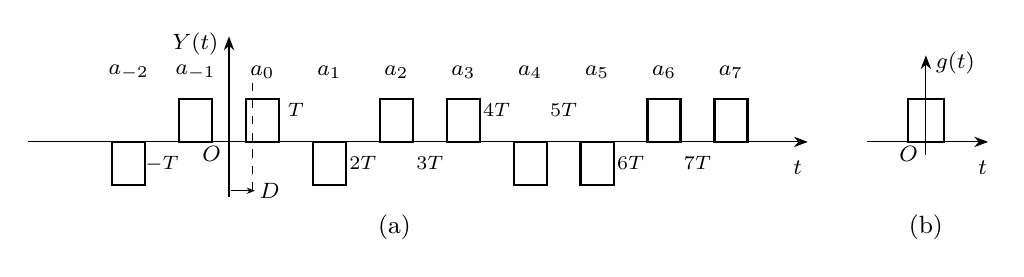
\begin{tikzpicture}[x=1cm,y=1cm,every node/.style={font=\footnotesize}]
  % ================= (a) Y(t) 方波序列 =================
  \draw[-{Stealth[length=5pt]}] (-2.55,0) -- (7.35,0);
  \node[below] at (7.22,-0.12) {$t$};
  \draw[-{Stealth[length=5pt]}] (0,-0.70) -- (0,1.34);
  \node[left,inner sep=2pt] at (-0.06,1.24) {$Y(t)$};
  \node[below left,inner sep=1pt] at (-0.06,-0.02) {$O$};
  % 各时隙内的方波脉冲（宽 0.42cm ≈ 0.5T；原书脉冲也明显窄于时隙，正负号与原书一致）
  \draw[thick] (-1.485,-0.55) -- (-1.485,0) -- (-1.065,0) -- (-1.065,-0.55) -- cycle;
  \draw[thick] (-0.635,0) -- (-0.635,0.55) -- (-0.215,0.55) -- (-0.215,0) -- cycle;
  \draw[thick] (0.215,0) -- (0.215,0.55) -- (0.635,0.55) -- (0.635,0) -- cycle;
  \draw[thick] (1.065,0) -- (1.065,-0.55) -- (1.485,-0.55) -- (1.485,0) -- cycle;
  \draw[thick] (1.915,0) -- (1.915,0.55) -- (2.335,0.55) -- (2.335,0) -- cycle;
  \draw[thick] (2.765,0) -- (2.765,0.55) -- (3.185,0.55) -- (3.185,0) -- cycle;
  \draw[thick] (3.615,0) -- (3.615,-0.55) -- (4.035,-0.55) -- (4.035,0) -- cycle;
  \draw[thick] (4.465,0) -- (4.465,-0.55) -- (4.885,-0.55) -- (4.885,0) -- cycle;
  \draw[thick] (5.315,0) -- (5.315,0.55) -- (5.735,0.55) -- (5.735,0) -- cycle;
  \draw[thick] (6.165,0) -- (6.165,0.55) -- (6.585,0.55) -- (6.585,0) -- cycle;
  % 时隙标号
  \node at (-1.275,0.88) {$a_{-2}$};
  \node at (-0.425,0.88) {$a_{-1}$};
  \node at (0.425,0.88) {$a_0$};
  \node at (1.275,0.88) {$a_1$};
  \node at (2.125,0.88) {$a_2$};
  \node at (2.975,0.88) {$a_3$};
  \node at (3.825,0.88) {$a_4$};
  \node at (4.675,0.88) {$a_5$};
  \node at (5.525,0.88) {$a_6$};
  \node at (6.375,0.88) {$a_7$};
  % 横轴上的时隙分界标号（4T、5T 在原书中标在轴上方）
  \node[below,font=\scriptsize] at (-0.85,-0.06) {$-T$};
  \node[above,font=\scriptsize] at (0.85,0.20) {$T$};
  \node[below,font=\scriptsize] at (1.70,-0.06) {$2T$};
  \node[below,font=\scriptsize] at (2.55,-0.06) {$3T$};
  \node[above,font=\scriptsize] at (3.40,0.20) {$4T$};
  \node[above,font=\scriptsize] at (4.25,0.20) {$5T$};
  \node[below,font=\scriptsize] at (5.10,-0.06) {$6T$};
  \node[below,font=\scriptsize] at (5.95,-0.06) {$7T$};
  % 随机滑动量 D：竖直虚线与双箭头标注
  \draw[dashed] (0.30,-0.62) -- (0.30,0.92);
  % 原书是"两段式"尺寸标注：左箭头指纵轴、右箭头指 D 的竖直虚线，D 标在右侧
  \draw[-{Stealth[length=3pt]}] (0.02,-0.62) -- (0.33,-0.62);
  \node[right,inner sep=1.5pt] at (0.33,-0.62) {$D$};
  \node at (2.10,-1.08) {\small (a)};
  % ================= (b) 单个脉冲 g(t) =================
  \draw[-{Stealth[length=5pt]}] (8.10,0) -- (9.64,0);
  \node[below] at (9.57,-0.12) {$t$};
  \draw[-{Stealth[length=5pt]}] (8.85,-0.16) -- (8.85,1.10);
  \node[right,inner sep=2pt] at (8.90,1.00) {$g(t)$};
  \node[below left,inner sep=1pt] at (8.79,-0.02) {$O$};
  \draw[thick] (8.62,0) -- (8.62,0.55) -- (9.08,0.55) -- (9.08,0) -- cycle;
  \node at (8.85,-1.08) {\small (b)};
\end{tikzpicture}
\captionof{figure}{随机数字传输信号与传输脉冲}\label{fig:3.15}
\end{center}

一种典型的随机二进制传输信号\nobreak：考虑 $\{a_n\}$ 为二进制无关序列\nobreak，等概地取值 $+1$ 与 $-1$\nobreak；$g(t)$ 为中心在原点\nobreak、宽度为 $T$\nobreak、高度为 $1$ 的方波脉冲\nobreak。易知\nobreak，$m_a=0$\nobreak，$R_a[k]=\delta[k]$\nobreak，$G(\ju\omega)=\dfrac{2\sin(\omega T/2)}{\omega}$\nobreak。于是\nobreak，随机二进制传输信号的特性为\nobreak：$\E Y(t)=0$\nobreak，且由随后的定理 3.5 可得
\begin{equation}
\resizebox{\dimexpr\linewidth-4em\relax}{!}{$\displaystyle
R_Y(\tau)=\frac{1}{T}r_g(\tau)=\frac{1}{T}g(\tau)*g(\tau)=
\begin{cases}
1-\lvert\tau\rvert/T, & \lvert\tau\rvert\leqslant T\\
0, & \lvert\tau\rvert>T
\end{cases}$}
\label{eq:3.34}
\end{equation}
\begin{equation}
\resizebox{\dimexpr\linewidth-4em\relax}{!}{$\displaystyle
S_Y(\omega)=\frac{1}{T}\times\frac{2\sin(\omega T/2)}{\omega}\times\frac{2\sin(\omega T/2)}{\omega}
=\frac{4\sin^2(\omega T/2)}{\omega^2T}$}
\label{eq:3.35}
\end{equation}
自相关函数与功率谱如图~\ref{fig:3.16} 所示\nobreak。可见\nobreak，信号的主要部分集中在主瓣上\nobreak，可粗略认为其带宽 $F=1/T$ Hz\nobreak。$F$ 是二元数据时隙宽度的倒数\nobreak，通常称为数据率\nobreak。

% ---- 图3.16（框内：center + \captionof）----
\begin{center}
\begin{tikzpicture}[x=1cm,y=1cm,every node/.style={font=\footnotesize}]
  % ================= (a) 自相关函数 =================
  \draw[-{Stealth[length=5pt]}] (-2.75,0) -- (3.15,0);
  \node[below] at (3.09,-0.12) {$\tau$};
  \draw[-{Stealth[length=5pt]}] (0,-0.32) -- (0,1.28);
  \node[right,inner sep=2pt] at (0.04,1.14) {$R(\tau)$};
  \node[left,inner sep=1pt] at (-0.10,0.94) {$1$};
  \draw[thick] (-1.65,0) -- (0,1.00) -- (1.65,0);
  \node[below] at (-1.65,-0.06) {$-T$};
  \node[below] at (1.65,-0.06) {$+T$};
  \node at (0.20,-1.12) {\small (a) 自相关函数};
  % ================= (b) 功率谱 =================
  \draw[-{Stealth[length=5pt]}] (3.70,0) -- (8.50,0);
  \node[below] at (8.44,-0.12) {$\omega$};
  \draw[-{Stealth[length=5pt]}] (6.10,-0.12) -- (6.10,1.28);
  \node[right,inner sep=2pt] at (6.14,1.14) {$S_Y(\omega)$};
  % 主瓣与旁瓣：sin^2(.)/(.)^2，第一零点在 omega = ±2π/T（图中 ±0.95cm）。
  % 原书把旁瓣画得明显可见（示意）；真实 sinc^2 的第一旁瓣只有主瓣的 4.7%，
  % 照实画几乎看不见，故按原书示意把 |omega|>2π/T 的旁瓣幅度放大约 2.5 倍
  %（振幅在零点处切换，函数连续，不会出现跳变）。
  \draw[thick] plot[samples=160,domain=-2.40:-0.004]
     (\x+6.10,{(abs(\x)>0.95 ? 2.5 : 1)*(sin(deg(pi*(\x)/0.95))/(pi*(\x)/0.95))^2});
  \draw[thick] plot[samples=160,domain=0.004:2.40]
     (\x+6.10,{(abs(\x)>0.95 ? 2.5 : 1)*(sin(deg(pi*(\x)/0.95))/(pi*(\x)/0.95))^2});
  \node[below] at (5.15,-0.06) {$-\dfrac{2\pi}{T}$};
  \node[below=1pt] at (6.10,-0.02) {$O$};
  \node[below] at (7.05,-0.06) {$\dfrac{2\pi}{T}$};
  \node at (6.20,-1.12) {\small (b) 功率谱};
\end{tikzpicture}
\captionof{figure}{随机二元（二进制\nobreak）传输信号的自相关函数与功率谱}\label{fig:3.16}
\end{center}

\end{examplebox}

数字电路中也常常遇到二进制传输信号\nobreak。比如同步电路中\nobreak，D 型触发器的 Q 输出端上的信号在时钟控制下逐时隙（时钟周期\nobreak）地送出\nobreak。当触发器的输入信号无法预知时\nobreak，我们常用随机二进制传输信号来描述 Q 端的输出信号\nobreak，并借助图~\ref{fig:3.16}\fw{b}分析信号的功率谱与带宽\nobreak。功率谱中只考虑主瓣一般是不够的\nobreak，还需要考虑几个明显非零的旁瓣\nobreak。假设时钟频率为 $F_{\text{clk}}=1/T$\nobreak，为了保持信号波形基本完整\nobreak，实际工程中通常需要至少 $3\sim5$ 倍的 $F_{\text{clk}}$ 的带宽\nobreak。

\thm{定理 3.5} 假定 $\{a_n\}$ 为平稳序列\nobreak，均值为 $m_a$\nobreak，自相关函数为 $R_a[k]$\nobreak。记 $g(t)$ 的傅里叶变换为 $G(\ju\omega)$\nobreak，则 $Y(t)$ 是平稳信号\nobreak，并且
\begin{citemize}
\item \fw{1}均值
\begin{equation}
\E Y(t)=\frac{m_a}{T}G(\ju 0)
\label{eq:3.36}
\end{equation}
\item \fw{2}自相关函数
\begin{equation}
R_Y(\tau)=\frac{1}{T}\sum_{k=-\infty}^{+\infty}R_a[k]r_g(\tau-kT)
\label{eq:3.37}
\end{equation}
\item \fw{3}功率谱
\begin{equation}
S_Y(\omega)=\frac{1}{T}\bigl\lvert G(\ju\omega)\bigr\rvert^{2}\sum_{k=-\infty}^{+\infty}R_a[k]\eu^{-\ju k\omega T}
\label{eq:3.38}
\end{equation}
\end{citemize}
其中
\[
r_g(\tau)=\int_{-\infty}^{+\infty}g(t+\tau)g(t)\dif t=g(\tau)*g(-\tau)
\]
\textbf{证明\nobreak：}\fw{1}由于 $X(t-D)$ 由随机序列 $\{a_n\}$ 与随机变量 $D$ 复合构成\nobreak，直接计算其均值不容易\nobreak。下面借助条件平均方法\nobreak，先考虑
\[
\E[X(t-D)\,|\,D=x]=\sum_{n=-\infty}^{+\infty}\E(a_n)g(t-nT-x)=m_a\sum_{n=-\infty}^{+\infty}g(t-nT-x)
\]

% EQNUMBERS: 3.33, 3.34, 3.35, 3.36, 3.37, 3.38
% FIGNUMBERS: 3.13, 3.14, 3.15, 3.16
% PAGES: 81-82

% =====================================================================
%  frag_H —— 书 p.83–84（PDF p.97–98）
%  内容：定理3.5 的证明（续）——(1) 均值收尾、(2) 自相关函数、(3) 功率谱；
%        例3.16（随机电报信号）题面（p.83 页末起，灰底框开在本片）、
%        图3.17、(3.39)、(3.40)、(3.41) 及全解（整页 p.84 都在框内，框在本片末闭合）
%  本片编号公式：(3.39)(3.40)(3.41)；图3.17（在灰底框内，用 center + \captionof）
%  灰底框：例3.16 —— \begin{examplebox} 与 \end{examplebox} 各一次，两端都在本片内
%  接缝：frag_G 停在 p.82 页末，本片从 p.83 的"于是…"起笔，**是新的段落**，不是同段接缝。
%        本片正常收尾（p.84 末句"…则信号的带宽也越宽。"完整），frag_I 从 p.85 习题起笔。
%  原书笔误：p.84 解里写"利用式（3.40）与全概率公式可计算出"，而此处刚给出的是 (3.39)
%            —— 原样保留，见下方该行注释。
% =====================================================================

\[
\begin{aligned}
\text{于是}\quad EY(t)&=\E\left[m_a\sum_{n=-\infty}^{+\infty}g(t-nT-D)\right]
      =\frac{m_a}{T}\sum_{n=-\infty}^{+\infty}\int_0^T g(t-nT-x)\dif x\\
&=\frac{m_a}{T}\int_{-\infty}^{+\infty}g(u)\dif u=\frac{m_a}{T}G(\ju 0)
\end{aligned}
\]

\fw{2}仿上\nobreak，借助条件平均方法计算自相关函数\nobreak。先考虑\nobreak，
% 本式逐行对齐、天然宽于版心，按第1章式(1.17) 先例等比压到版心内（仍是矢量文字）
\[
\resizebox{\linewidth}{!}{$\displaystyle
\begin{aligned}
\E\bigl[Y(t+\tau)Y(t)\big|D=x\bigr]&=\E\left[\sum_{n=-\infty}^{+\infty}a_ng(t+\tau-nT-x)\sum_{m=-\infty}^{+\infty}a_mg(t-mT-x)\right]\\
&=\sum_{n=-\infty}^{+\infty}\sum_{m=-\infty}^{+\infty}\left\{\E[a_na_m]g(t+\tau-nT-x)g(t-mT-x)\right\}\\
&=\sum_{k=-\infty}^{+\infty}\left\{R_a[k]\sum_{m=-\infty}^{+\infty}g(t+\tau-mT-kT-x)g(t-mT-x)\right\}
\end{aligned}$}
\]

其中令 $k=n-m$\nobreak，并更换了求和变量\nobreak。于是
% 本式逐行对齐、天然宽于版心，按第1章式(1.17) 先例等比压到版心内
\[
\resizebox{\linewidth}{!}{$\displaystyle
\begin{aligned}
R_Y(t+\tau,t)&=\E\left\{\sum_{k=-\infty}^{+\infty}\left\{R_a[k]\sum_{m=-\infty}^{+\infty}g(t+\tau-mT-kT-D)g(t-mT-D)\right\}\right\}\\
&=\frac{1}{T}\sum_{k=-\infty}^{+\infty}\left\{R_a[k]\sum_{m=-\infty}^{+\infty}
  \left[\int_{-T/2}^{T/2}g(t+\tau-mT-kT-x)g(t-mT-x)\dif x\right]\right\}
\end{aligned}$}
\]

对于上式中的和式部分\nobreak，令 $u=t-mT-x$\nobreak，有
\[
\begin{aligned}
\sum_{m=-\infty}^{+\infty}\int_{-T/2-mT+t}^{T/2-mT+t}g(u+\tau-kT)g(u)\dif u
  &=\int_{-\infty}^{+\infty}g(u+\tau-kT)g(u)\dif u\\
&=r_g(\tau-kT)
\end{aligned}
\]

% 原书"于是"在左边距、与公式同行
\[
\text{于是}\quad R_Y(t+\tau,t)=R_Y(\tau)=\frac{1}{T}\sum_{k=-\infty}^{+\infty}R_a[k]r_g(\tau-kT)
\]

可见\nobreak，$Y(t)$是平稳信号\nobreak。

\fw{3}下面计算功率谱\nobreak。容易看出
\[
R_Y(\tau)=\frac{1}{T}\left\{\sum_{k=-\infty}^{+\infty}R_a[k]\delta(\tau-kT)\right\}*r_g(\tau)
\]
其中\nobreak，卷积的前一项是冲激串形式\nobreak，而 $r_g(\tau)\longleftrightarrow\lvert G(\ju\omega)\rvert^2$\nobreak，于是\nobreak，根据傅里叶变换的基本性质易知
\[
S_Y(\omega)=\lvert G(\ju\omega)\rvert^2\cdot\frac{1}{T}\sum_{k=-\infty}^{+\infty}R_a[k]\eu^{-\ju k\omega T}
\]
其实\nobreak，从例 3.5 中我们看到半随机二进制传输信号 $X(t)$ 是严格循环平稳的\nobreak，因此\nobreak，经过随机抖动后\nobreak，$Y(t)=X(t-D)$ 是严格平稳的\nobreak。利用有关定理也可以计算出其自相关函数与功率谱\nobreak。

\begin{examplebox}
\textbf{例3.16}\quad 讨论（取值$\pm1$的\nobreak）随机电报信号的平稳性与功率谱\nobreak。

随机电报信号\fw{Random Telegraph Signal}$X(t)$是一种随机的两电平信号\nobreak，定义如下\nobreak：

①在 $t=0$ 的初始时刻\nobreak，$X(0)$ 取值可为 $+1$ 或 $-1$\nobreak，概率分别为 $1/2$\nobreak；②而后\nobreak，在任何 $[0,t)$ 上\nobreak，$X(t)$ 在 0 与 1 之间以“泊松特性”发生随机翻转\nobreak，翻转与初值独立\nobreak，翻转次数 $N(t)$ 服从泊松分布 $P(\lambda t)$\nobreak。它的典型样本如图~\ref{fig:3.17} 所示\nobreak。

\begin{center}
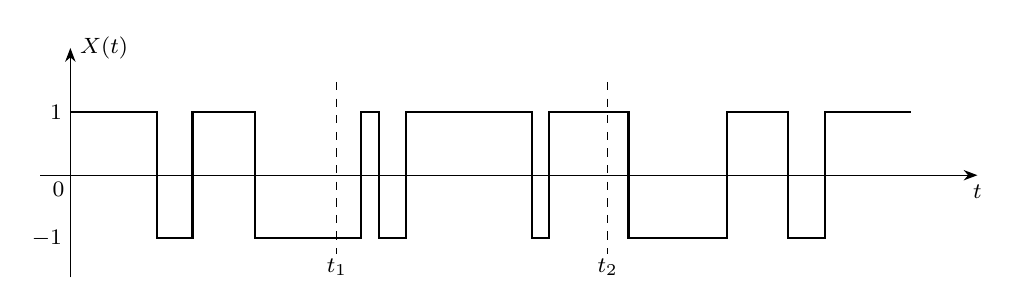
\begin{tikzpicture}[x=0.80cm,y=0.80cm,every node/.style={font=\footnotesize}]
  % ---- 坐标轴 ----
  \draw[-{Stealth[length=5pt]}] (0,-1.62) -- (0,2.02) node[right] {$X(t)$};
  \draw[-{Stealth[length=5pt]}] (-0.48,0) -- (14.40,0) node[below] {$t$};
  % ---- 电平标注 1 / 0 / -1 ----
  \node[left,inner sep=1.5pt] at (-0.06,1) {$1$};
  \node[below left,inner sep=1.5pt] at (-0.02,-0.04) {$0$};
  \node[left,inner sep=1.5pt] at (-0.06,-1) {$-1$};
  % ---- t1、t2 处的竖直虚线 ----
  \draw[dashed,thin] (4.23,1.48) -- (4.23,-1.25);
  \draw[dashed,thin] (8.53,1.48) -- (8.53,-1.25);
  \node[below,inner sep=1.5pt] at (4.23,-1.25) {$t_1$};
  \node[below,inner sep=1.5pt] at (8.53,-1.25) {$t_2$};
  % ---- 取值 ±1 的随机方波（X(0)=1，翻转时刻随机）----
  \draw[thick] (0,1) -- (1.37,1) -- (1.37,-1) -- (1.94,-1) -- (1.94,1)
    -- (2.93,1) -- (2.93,-1) -- (4.61,-1) -- (4.61,1) -- (4.90,1)
    -- (4.90,-1) -- (5.33,-1) -- (5.33,1) -- (7.33,1) -- (7.33,-1)
    -- (7.60,-1) -- (7.60,1) -- (8.86,1) -- (8.86,-1) -- (10.42,-1)
    -- (10.42,1) -- (11.39,1) -- (11.39,-1) -- (11.98,-1) -- (11.98,1)
    -- (13.35,1);
\end{tikzpicture}
\captionof{figure}{随机电报信号样本函数示例（$X(0)$ 为 1 的情形\nobreak）}\label{fig:3.17}
\end{center}

考虑在 $\pm1$（伏特\nobreak）的电平间进行随机选择的试验\nobreak：初始时刻的电平是随机的\nobreak，而后又发生随机翻转\nobreak，每单位时间平均翻转 $\lambda$ 次\nobreak，位置不定\nobreak，但服从泊松信号的特性\nobreak。显然有
\begin{equation}
\begin{cases}
X(t)=+X(0), & \text{若 $N(t)$ 为偶数}\\
X(t)=-X(0), & \text{若 $N(t)$ 为奇数}
\end{cases}
\label{eq:3.39}
\end{equation}

有时\nobreak，随机电报信号也可以表示为 $\{X(t)=A(-1)^{N(t)},t\geqslant0\}$\nobreak，其中 $\{N(t),t\geqslant0\}$ 是常数为 $\lambda$ 的泊松计数信号\nobreak，$A$ 为等概的（$+1$\nobreak，$-1$\nobreak）二元随机变量\nobreak。

\textbf{解\nobreak：}\quad 利用式\fw{3.40}与全概率公式可计算出  % 原书如此（疑似笔误\nobreak：此处应为 (3.39)\nobreak）
\[
\resizebox{\linewidth}{!}{$\displaystyle
\begin{aligned}
P[X(t)=1]&=P[X(t)=1|X(0)=1]\times P[X(0)=1]+P[X(t)=1|X(0)=-1]\times P[X(0)=-1]\\
&=P[N(t)\text{为偶数}|X(0)=1]\times\frac{1}{2}+P[N(t)\text{为奇数}|X(0)=-1]\times\frac{1}{2}\\
&=P[N(t)\text{为偶数}]\times\frac{1}{2}+P[N(t)\text{为奇数}]\times\frac{1}{2}\\
&=1/2
\end{aligned}$}
\]
\[
P[X(t)=-1]=1-P[X(t)=1]=1/2
\]
可见\nobreak，该信号在任何时刻的取值都是二元等概的\nobreak。所以
\[
m(t)=\E[X(t)]=1/2-1/2=0
\]
计算其自相关函数时\nobreak，不妨先考虑 $t_2\geqslant t_1$\nobreak，有
\[
\resizebox{\linewidth}{!}{$\displaystyle
\begin{aligned}
R(t_1,t_2)&=\E[X(t_1)X(t_2)]=1\times P[X(t_1)X(t_2)\text{同号}]+(-1)\times P[X(t_1)X(t_2)\text{反号}]\\
&=P[N(t_2-t_1)\text{为偶数}]-P[N(t_2-t_1)\text{为奇数}]\\
&=2P[N(t_2-t_1)\text{为偶数}]-1
\end{aligned}$}
\]
式中\nobreak，$N(t_2-t_1)$ 是在 $t_1$ 至 $t_2$ 期间发生的翻转次数\nobreak。于是\nobreak，令 $\tau=t_2-t_1$\nobreak，有
\[
\begin{aligned}
P[N(\tau)\text{为偶数}]&=\sum_{\substack{k=0\\ k\text{为偶数}}}^{\infty}
  \frac{(\lambda\tau)^k\eu^{-\lambda\tau}}{k!}
  =\frac{\eu^{-\lambda\tau}}{2}\sum_{n=0}^{\infty}
  \left[\frac{(\lambda\tau)^n}{n!}+\frac{(-\lambda\tau)^n}{n!}\right]\\
&=\frac{\eu^{-\lambda\tau}}{2}\left(\eu^{\lambda\tau}+\eu^{-\lambda\tau}\right)
  =\left(1+\eu^{-2\lambda\tau}\right)/2
\end{aligned}
\]
\[
\text{因此}\quad R(\tau)=2\times\left(1+\eu^{-2\lambda\tau}\right)/2-1=\eu^{-2\lambda\tau}
\]
考虑到 $t_2,t_1$ 的一般情况\nobreak，利用对称性\nobreak，最后有
\begin{equation}
R(\tau)=\eu^{-2\lambda\lvert\tau\rvert}
\label{eq:3.40}
\end{equation}

可见\nobreak，随机电报信号是广义平稳的\nobreak。利用傅里叶变换对\nobreak：$\eu^{-a\lvert t\rvert}\leftrightarrow\frac{2a}{\omega^2+a^2}$\nobreak，得到功率谱为
\begin{equation}
S(\omega)=\frac{4\lambda}{\omega^2+4\lambda^2}
\label{eq:3.41}
\end{equation}
它说明该信号主要由低频成分构成\nobreak。容易看出\nobreak，其 3 dB 带宽为 $B=2\pi\times2\lambda$ Hz\nobreak，因此\nobreak，翻转的平均率 $\lambda$ 越大\nobreak，则信号的带宽也越宽\nobreak。
\end{examplebox}

% EQNUMBERS: 3.39, 3.40, 3.41
% FIGNUMBERS: 3.17
% PAGES: 83-84

% =====================================================================
%  frag_I —— 《随机信号分析（第5版）》书 p.85–86（PDF p.99–100）
%  内容：① 3.6 节正文收尾段（随机电报信号，p.85 页首整段）
%        ②  + \exhead{习题}（原书 p.85 居中加粗「习题」两字）
%        ③ 习题 3.1 – 3.11（p.85）、3.12 – 3.21（p.86）
%  本片编号公式：无（习题区原书一律不给公式号，全部用 \[ \] 或行内 $...$）
%  本片题图：无（题图 图题3.33、图题3.34 都在 p.88，属 frag_J）
%  ★ 接缝：本片从 p.85 页首那段正文起笔（不是从句中接）；
%    尾行 = p.86 页末 3.21 的 (3) 项；3.21 的 (4)(5)(6) 在 frag_J 续写，
%    两边各用一个 subqthree，**不要**重复 3.21 的题面。
%  排版注记（子问题布局——以扫描页印刷为准）：
%    · 3.1 / 3.2 / 3.7 的子问题在原书中**竖排**（各自单独成行、带缩进）→ citemize；
%    · 3.3 / 3.8 / 3.13 / 3.14 / 3.17 / 3.18 / 3.19 / 3.20 的子问题在原书中
%      排成**两栏**（同一行左右各一项）→ subq（每格加 \sqr = \rightskip 0pt plus 1fil，
%      避免 p 栏里因 \emergencystretch 拉出大空隙；不用 \raggedright，它会重定义 \\）；
%    · 3.5 的 (1)(2)(3) 与 3.21 的 (1)(2)(3) 每行 3 项：3.21 用 subqthree；
%      3.5 三项总宽 ≈ 版心宽（375.8pt vs 375.6pt），用 subqthree 会把第三项挤成
%      两行，故照原书"左右铺开"的样子写成一行 + \hfill（装配时 \fw 化后总宽 343pt 可容纳）；
%    · 3.9 的 (1)(2)(3) 在原书中是**连排的一段**（跨行流动，不是分栏）→ 普通段落。
% =====================================================================

% 子问题两栏排版里把 \rightskip 设为 ragged（不用 \raggedright：它会重定义 \\，
% 把 tabular 的行分隔符改坏）。
\providecommand{\sqr}{\rightskip=0pt plus 1fil\relax}

随机电报信号在异步数字电路中可能遇到\nobreak。比如\nobreak，某 T 型触发器的输出信号受触发电平控制\nobreak，在高低电平之间来回翻转\nobreak。我们无法预知下一次触发何时到来\nobreak，认为触发边沿之间的间距是随机的\nobreak，并常常简单地认为这种间距服从均值为某 $\lambda$ 的指数分布\nobreak。可以证明\nobreak，这时的翻转特性正是参数为 $\lambda$ 的泊松分布\nobreak，因此\nobreak，触发器的输出信号就可以用随机电报信号来描述\nobreak。

\exhead{习题}

\exer{3.1}随机电压信号 $U(t)$ 在各不同时刻上是统计独立的\nobreak，而且\nobreak，其一阶概率密度函数是高斯的\nobreak，均值为 0\nobreak，方差为 2\nobreak。试求\nobreak：

\begin{citemize}
\item \fw{1}密度函数 $f(u;t)$\nobreak，$f(u_1,u_2;t_1,t_2)$ 和 $f(u_1,u_2,\cdots,u_k;t_1,t_2,\cdots,t_k)$\nobreak，$k$ 为任意整数\nobreak；
\item \fw{2}$U(t)$ 的平稳性\nobreak。
\end{citemize}

\exer{3.2}若随机信号 $X(t)$ 的二阶概率密度函数有如下关系
\[
f_X(x_1,x_2;t_1,t_2)=f_X(x_1,x_2;t_1+\Delta,t_2+\Delta)
\]
式中\nobreak，$\Delta$ 为任意值\nobreak。试证明\nobreak：

\begin{citemize}
\item \fw{1}$X(t)$ 的一阶概率密度函数 $f_X(x_1;t_1)=f_X(x_1;t_1+\Delta)$\nobreak；
\item \fw{2}$X(t)$ 的均值 $m_X(t)=m_X(t+\Delta)$\nobreak；
\item \fw{3}$X(t)$ 的相关函数 $E[X(t+\tau)X(t)]=R_X(\tau)$\nobreak。
\end{citemize}

\exer{3.3}随机过程由下述三个样本函数组成\nobreak，且等概率发生\nobreak：
\[
X(t,\xi_1)=1,\quad X(t,\xi_2)=\sin t,\quad X(t,\xi_3)=\cos t
\]
\begin{subq}\setlength{\parindent}{0pt}
\sqr\fw{1}计算均值 $m_X(t)$ 和自相关函数 $R_X(t_1,t_2)$\nobreak； & \sqr\fw{2}该随机过程 $X(t)$ 是否平稳\nobreak？
\end{subq}

\exer{3.4}已知随机信号 $X(t)$ 和 $Y(t)$ 相互独立且各自平稳\nobreak，证明随机信号 $Z(t)=X(t)Y(t)$ 也是平稳的\nobreak。

\exer{3.5}随机信号 $X(t)=10\sin(\omega_0t+\Theta)$\nobreak，$\omega_0$ 为确定常数\nobreak，$\Theta$ 为在 $[-\pi,\pi]$ 上均匀分布的随机变量\nobreak。若 $X(t)$ 通过平方律器件\nobreak，得到 $Y(t)=X^2(t)$\nobreak，试求\nobreak：

% 3.5 的 (1)(2)(3) 在原书中排成一行、左右铺开；三项连排总宽 ≈ 版心宽（装配 \fw 化后 343pt），
% 用 subqthree 会把第三项挤成两行，故写成一行 + \hfill。
\noindent \fw{1}$Y(t)$ 的均值\nobreak；\hfill\fw{2}$Y(t)$ 的相关函数\nobreak；\hfill\fw{3}$Y(t)$ 的广义平稳性\nobreak。

\exer{3.6}给定随机过程 $X(t)=A\cos(\omega_0t)+B\sin(\omega_0t)$\nobreak，其中 $\omega_0$ 是常数\nobreak，$A$ 和 $B$ 是两个任意的不相关随机变量\nobreak，它们的均值为零\nobreak，方差同为 $\sigma^2$\nobreak。证明 $X(t)$ 是广义平稳而不是严格平稳的\nobreak。

\exer{3.7}$Y(t)$ 是广义循环平稳的实随机信号\nobreak，循环周期为 100\nobreak，均值 $m(10)=20$\nobreak，相关函数 $R(5,1)=10$\nobreak。求\nobreak：

\begin{citemize}
\item \fw{1}$E[5Y(110)]$\nobreak，$E[10Y(310)+50]$\nobreak；
\item \fw{2}$E[Y(105)Y(101)]$\nobreak，$E[30Y(205)Y(201)+200]$\nobreak；
\item \fw{3}$E[10Y(305)Y(301)+6Y(210)+80]$\nobreak。
\end{citemize}

\exer{3.8}给定过程 $X(t)=A\cos t-B\sin t$ 和 $Y(t)=B\cos t+A\sin t$\nobreak，其中随机变量 $A,B$ 独立\nobreak，均值都为 0\nobreak，方差都为 5\nobreak。

\begin{subq}\setlength{\parindent}{0pt}
\sqr\fw{1}证明 $X(t)$ 和 $Y(t)$ 各自平稳且联合平稳\nobreak； & \sqr\fw{2}求两个过程的互相关函数\nobreak。
\end{subq}

\exer{3.9}两个统计独立的平稳随机过程 $X(t)$ 和 $Y(t)$\nobreak，其均值都为 0\nobreak，自相关函数分别为
\[
R_X(\tau)=\eu^{-\lvert\tau\rvert},\quad R_Y(\tau)=\cos 2\pi\tau
\]
\fw{1}求 $Z(t)=X(t)+Y(t)$ 的自相关函数\nobreak；\fw{2}求 $W(t)=X(t)-Y(t)$ 的自相关函数\nobreak；\fw{3}互相关函数 $R_{ZW}(\tau)$\nobreak。

\exer{3.10}已知平稳高斯信号 $X(t)$ 的均值为 0\nobreak，令 $Y(t)=X^2(t)$\nobreak。证明\nobreak：$R_Y(\tau)=[R_X(0)]^2+2[R_X(\tau)]^2$\nobreak。

\exer{3.11}设平稳高斯信号 $X(t)$ 的均值为零\nobreak，自相关函数为 $R_X(\tau)=\sin(\pi\tau)/\pi\tau$\nobreak，求 $t_1=0$\nobreak，$t_2=0.5$ 与 $t_3=1$ 时的三维概率密度\nobreak。

\exer{3.12}广义平稳随机过程 $Y(t)$ 的自相关函数矩阵如下\nobreak，试确定矩阵中带下画线的空白处元素的值\nobreak。
\[
\begin{bmatrix}
2 & 1.3 & 0.4 & \underline{\hspace{1.2em}}\\
\underline{\hspace{1.2em}} & 2 & 1.2 & 0.8\\
0.4 & 1.2 & \underline{\hspace{1.2em}} & 1.1\\
0.9 & \underline{\hspace{1.2em}} & \underline{\hspace{1.2em}} & 2
\end{bmatrix}
\]
% 上矩阵照原书逐格抄录。空白处（下画线）为待填元素，共 5 处：
% (1,4) (2,1) (3,3) (4,2) (4,3)。原书 (3,3) 这个对角元素也留空，原样保留。

\exer{3.13}已知平稳信号 $X(t)$ 的自相关函数为

\begin{subq}\setlength{\parindent}{0pt}
\sqr\fw{1}$R_X(\tau)=6\exp(-\lvert\tau\rvert/2)$\nobreak； & \sqr\fw{2}$R_X(\tau)=6\dfrac{\sin\pi\tau}{\pi\tau}$
\end{subq}
对于任意给定的 $t$\nobreak，求信号四个状态 $X(t),X(t+1),X(t+2),X(t+3)$ 的协方差矩阵\nobreak。

\exer{3.14}对于两个零均值广义平稳随机过程 $X(t)$ 和 $Y(t)$\nobreak，已知 $\sigma_X^2=5$\nobreak，$\sigma_Y^2=10$\nobreak，问下述函数可否作为自相关函数\nobreak？为什么\nobreak？

\begin{subq}\setlength{\parindent}{0pt}
\sqr\fw{1}$R_X(\tau)=5u(\tau)\exp(-3\tau)$\nobreak； & \sqr\fw{2}$R_X(\tau)=5\sin(5\tau)$\nobreak；\\
\sqr\fw{3}$R_Y(\tau)=9(1+2\tau^2)^{-1}$\nobreak； & \sqr\mbox{\fw{4}$R_Y(\tau)=-\cos(6\tau)\exp(-\lvert\tau\rvert)$\nobreak；}\\
\sqr\fw{5}$R_X(\tau)=5\left[\dfrac{\sin 3\tau}{3\tau}\right]^2$\nobreak； & \sqr\fw{6}$R_Y(\tau)=6+4\left[\dfrac{\sin 10\tau}{10\tau}\right]$\nobreak；\\
\sqr\fw{7}$R_X(\tau)=5\exp(-\lvert\tau\rvert)$\nobreak； & \sqr\fw{8}$R_Y(\tau)=6+4\exp(-3\tau^2)$\nobreak。
\end{subq}

\exer{3.15}已知平稳过程 $X(t)$ 的自相关函数为 $R_X(\tau)=4\eu^{-\lvert\tau\rvert}\cos\pi\tau+\cos 3\pi\tau$\nobreak，求过程 $X(t)$ 的均方值和方差\nobreak。

\exer{3.16}已知随机过程 $X(t)$ 和 $Y(t)$ 独立且各自平稳\nobreak，自相关函数为 $R_X(\tau)=2\eu^{-\lvert\tau\rvert}\cos\omega_0\tau$\nobreak，$R_Y(\tau)=9+\exp(-3\tau^2)$\nobreak。令随机过程 $Z(t)=AX(t)Y(t)$\nobreak，其中 $A$ 是均值为 2\nobreak、方差为 9 的随机变量\nobreak，且与 $X(t)$ 和 $Y(t)$ 相互独立\nobreak。求过程 $Z(t)$ 的均值\nobreak、方差和自相关函数\nobreak。

\exer{3.17}设 $X(t)$ 与 $Y(t)$ 是联合平稳的\nobreak，试证明\nobreak：

\begin{subq}\setlength{\parindent}{0pt}
\sqr\fw{1}$\lvert R_{XY}(\tau)\rvert\leqslant\sqrt{R_X(0)R_Y(0)}$ & \sqr\mbox{\fw{2}$\lvert R_{XY}(\tau)\rvert\leqslant[R_X(0)+R_Y(0)]/2$}
\end{subq}
（提示\nobreak：利用 $E[\lvert X(t+\tau)-\alpha Y(t)\rvert^2]\geqslant0$\nobreak）

\exer{3.18}已知平稳随机过程的相关函数为\nobreak：

\begin{subq}\setlength{\parindent}{0pt}
\sqr\fw{1}$R_X(\tau)=\sigma_X^2\eu^{-a\lvert\tau\rvert}$ & \sqr\fw{2}$R_X(\tau)=\sigma_X^2(1-a\lvert\tau\rvert)$\nobreak，$\lvert\tau\rvert\leqslant1/a$
\end{subq}
试求它们的相关时间 $\tau_0$\nobreak。

\exer{3.19}平稳信号 $X(t)$ 的功率谱密度为\nobreak：

\begin{subq}\setlength{\parindent}{0pt}
\sqr\fw{1}$S_X(\omega)=\dfrac{\omega^2}{\omega^4+3\omega^2+2}$ & \sqr\fw{2}$S_X(\omega)=\begin{cases}8\delta(\omega)+20(1-\lvert\omega\rvert/10), & \lvert\omega\rvert\leqslant10\\ 0, & \lvert\omega\rvert>10\end{cases}$
\end{subq}
\fw{3}$S_X(\omega)=p\cos^4\omega\tau_0$\nobreak，$p$ 为常数

求它们的自相关函数和均方值\nobreak。

\exer{3.20}已知平稳信号 $X(t)$ 的自相关函数为\nobreak：

\begin{subq}\setlength{\parindent}{0pt}
\sqr\fw{1}$R(\tau)=\eu^{-3\lvert\tau\rvert}$ & \sqr\fw{2}$R(\tau)=5\eu^{-\tau^2/8}$\\
\sqr\mbox{\fw{3}$R(\tau)=4\eu^{-\lvert\tau\rvert}\cos\pi\tau+\cos 3\pi\tau$} & \sqr\fw{4}$R(\tau)=\begin{cases}1-\lvert\tau\rvert, & \tau\leqslant1\\ 0, & \tau>1\end{cases}$
\end{subq}
求它们的功率谱密度\nobreak。

\exer{3.21}下述函数哪些是实随机信号功率谱的正确表达式\nobreak？为什么\nobreak？

% ↓ 本行 (1)(2)(3) 在原书 p.86 页末；其 (4)(5)(6) 在 p.87 页首，由 frag_J 续写
\begin{subqthree}\setlength{\parindent}{0pt}
\sqr\fw{1}$\left(\dfrac{\sin\omega}{\omega}\right)^2$ & \sqr\fw{2}$\dfrac{\omega^2}{\omega^6+3\omega^2+3}$ & \sqr\fw{3}$\dfrac{\omega^2}{\omega^4-1}-\delta(\omega)$
\end{subqthree}

% EQNUMBERS: （无）
% FIGNUMBERS: （无）
% PAGES: 85-86
% EXERCISES: 3.1 3.2 3.3 3.4 3.5 3.6 3.7 3.8 3.9 3.10 3.11
%            3.12 3.13 3.14 3.15 3.16 3.17 3.18 3.19 3.20 3.21
%            （连续无跳号；3.21 的 (1)(2)(3) 为 p.86 末行，(4)(5)(6) 续于 frag_J）

% =====================================================================
%  frag_J —— 《随机信号分析（第5版）》书 p.87–88（PDF p.101–102）
%  内容：① 3.21 的 (4)(5)(6)（p.87 页首；题面与 (1)(2)(3) 已在 frag_I，**不重复**）
%        ② 习题 3.22 – 3.33（p.87）、3.34（p.88）
%        ③ 两张题图：图题3.33（矩形脉冲串）、图题3.34（锯齿波脉冲串），p.88
%  本片编号公式：无（习题区一律 \[ \] 或行内 $...$）
%  ★ 题图**独立编号**，不占正文 figure 计数器：用非浮动 center + TikZ + 手写图注
%    "图题3.33"/"图题3.34"（字面量，中间不插空格），不用 \caption、不用
%    \refstepcounter（否则正文 图3.x 全乱）。
%  ★ 接缝：本片第一行就是 3.21 的 (4)(5)(6) 行；**不要**再写 3.21 题面、不要 \exhead。
%  排版注记：3.21 (4)(5)(6) 用 subqthree（与 frag_I 里的 (1)(2)(3) 同一环境、同一栏宽）；
%    3.29 的 (1)(2) 原书竖排 → citemize；3.30 的 (1)(2) 同一行两栏 → subq。
% =====================================================================

% 子问题两栏/三栏里把 \rightskip 设为 ragged（不用 \raggedright：它会重定义 \\，
% 把 tabular 的行分隔符改坏）。frag_I 里已定义则此处不重复定义。
\providecommand{\sqr}{\rightskip=0pt plus 1fil\relax}

% ↓ 3.21 的 (4)(5)(6)（书 p.87 第一行；题面见 frag_I，不重复）
\begin{subqthree}\setlength{\parindent}{0pt}
\sqr\fw{4}$\dfrac{\omega^4}{j\omega^6+\omega^2+1}$ & \sqr\fw{5}$\dfrac{\lvert\omega\rvert}{\omega^4+2\omega^2+1}$ & \sqr\fw{6}$\eu^{-(\omega-1)^2}$
\end{subqthree}

\exer{3.22}在附录 A“傅里叶变换性质与常用变换对”表格中\nobreak，从序号 13$\sim$34\nobreak，哪些变换对可作为平稳信号的一对自相关函数与功率谱\nobreak？

\exer{3.23}$X(t)$ 是平稳随机过程\nobreak，证明\nobreak：过程 $Y(t)=X(t+T)+X(t)$ 的功率谱为
\[
S_Y(\omega)=2S_X(\omega)(1+\cos\omega T)
\]

\exer{3.24}设 $X(t)$ 和 $Y(t)$ 是两个独立的平稳随机过程\nobreak，均值分别为常量 $m_X$ 和 $m_Y$\nobreak，且 $X(t)$ 的功率谱为 $G_X(\omega)$\nobreak，定义 $Z(t)=X(t)+Y(t)$\nobreak，试计算 $S_{XY}(\omega)$\nobreak，$S_{XZ}(\omega)$\nobreak。

\exer{3.25}设两个随机过程 $X(t)$ 和 $Y(t)$ 联合平稳\nobreak，其互相关函数为
\[
R_{XY}(\tau)=\begin{cases}
9\eu^{-3\tau}, & \tau\geqslant0\\
0, & \tau<0
\end{cases}
\]
求互谱密度 $S_{XY}(\omega)$ 与 $S_{YX}(\omega)$\nobreak。

\exer{3.26}设随机过程 $X(t)=\sum\limits_{i=1}^{n}a_iX_i(t)$\nobreak，式中 $a_i$ 是一组实常数\nobreak。而随机过程 $X_i(t)$ 为平稳的和彼此正交的\nobreak。

试证明\nobreak：$S_X(\omega)=\sum\limits_{i=1}^{n}a_i^2S_{X_i}(\omega)$\nobreak。

\exer{3.27}设 $S_X(\omega)$ 是一个随机过程的功率谱密度函数\nobreak，证明 $\dif^2S_X(\omega)/\dif\omega^2$ 不可能是功率谱密度函数\nobreak。

\exer{3.28}设 $X(t)$ 和 $Y(t)$ 联合平稳\nobreak。试证明\nobreak：
\[
\Rre\{S_{XY}(\omega)\}=\Rre\{S_{YX}(\omega)\},\quad \Iim\{S_{XY}(\omega)\}=-\Iim\{S_{YX}(\omega)\}
\]

\exer{3.29}设 $X(t)$ 与 $Y(t)$ 是广义平稳信号\nobreak。试证明\nobreak：

\begin{citemize}
\item \fw{1}如果它们正交\nobreak，则 $S_{XY}(\omega)=0$\nobreak；
\item \fw{2}如果它们无关且均值都不为零\nobreak，则 $S_{XY}(\omega)=2\pi m_Xm_Y\delta(\omega)$\nobreak。
\end{citemize}

\exer{3.30}设 $U(t)$ 是网络产生的热噪声电压\nobreak，它具有平稳高斯分布\nobreak。假定 $RC=10^{-3}\ \mathrm{s}$\nobreak，$C=3\times1.38\times10^{-9}\ \mathrm{F}$\nobreak，$T=300\ \mathrm{K}$（电阻的绝对温度\nobreak）\nobreak，并知热噪声电压的自相关函数为
% 原书如此（疑似笔误）：$C=3\times1.38\times10^{-9}$ F，疑为 $3\times10^{-9}$ F 之误，照原书保留。
\[
R_U(\tau)=\frac{kT}{C}\eu^{-\frac{\lvert\tau\rvert}{RC}}
\]
式中\nobreak，$k=1.38\times10^{-23}\ \mathrm{J}/\mathrm{K}$\nobreak，为玻耳兹曼常数\nobreak。试求\nobreak：

\begin{subq}\setlength{\parindent}{0pt}
\sqr\fw{1}热噪声电压的均值\nobreak、方差\nobreak； & \sqr\fw{2}在时刻 $t_1$ 处\nobreak，热噪声电压超过 $10^{-6}\ \mathrm{V}$ 的概率\nobreak。
\end{subq}

\exer{3.31}考虑取值 1 与 0 的（单极性\nobreak）随机二进制传输信号\nobreak，\allowbreak$Y(t)=\sum\limits_{n=-\infty}^{+\infty}a_ng_T(t-nT-D)$\nobreak。其中\nobreak，$\{a_n\}$ 为二进制无关序列\nobreak，等概地取值 1 与 0\nobreak；$D$ 在 $[0,T)$ 上均匀分布\nobreak，且与 $\{a_n\}$ 独立\nobreak；$g_T(t)$ 为中心在原点\nobreak、宽度为 $T$\nobreak、高度为 1 的方波脉冲\nobreak。求信号的功率谱\nobreak。

\exer{3.32}考虑取值 $+1$ 与 $-1$ 的随机二进制传输信号\nobreak，\allowbreak$Y(t)=\sum\limits_{n=-\infty}^{+\infty}a_ng_T(t-nT-D)$\nobreak。其中\nobreak，$\{a_n\}$ 为二进制无关序列\nobreak，取值 1 与 0 的概率分别是 $p$ 与 $q$（$p+q=1$\nobreak）\nobreak；$D$ 在 $[0,T)$ 上均匀分布\nobreak，且与 $\{a_n\}$ 独立\nobreak；$g_T(t)$ 为中心在原点\nobreak、宽度为 $T$\nobreak、高度为 1 的方波脉冲\nobreak。求信号的功率谱\nobreak。
% 原书如此（疑似笔误）：前句「取值 +1 与 -1」，后句「取值 1 与 0 的概率」，前后不一致，照原书保留。

\exer{3.33}随机过程 $X(t)$ 的样本函数如图题 3.33 所示\nobreak，它在 $t_0+nT$ 时刻是宽度为 $b$ 的矩形脉冲\nobreak，脉冲幅度以等概率取 $\pm a$\nobreak，$t_0$ 是在 $[0,T)$ 上均匀分布的随机变量\nobreak，而且 $t_0$ 与所有脉冲都统计独立\nobreak。求 $R_X(\tau)$ 及均方值 $E[X^2(t)]$\nobreak。

\exer{3.34}假定周期为 $T$\nobreak、高为 $A$ 的锯齿波脉冲串具有随机相位\nobreak，如图题 3.34 所示\nobreak，它在 $t=0$ 时刻以后出现的第一个零值时刻是在 $[0,T)$ 内均匀分布的随机变量\nobreak。试证明 $X(t)$ 的一阶密度函数为
\[
f(x;t)=\begin{cases}
1/A, & x\in[0,A]\\
0, & x\notin[0,A]
\end{cases}
\]

% =====================================================================
%  两张题图（p.88）：图题3.33 在左、图题3.34 在右，并排；非浮动、不占 figure 计数器
% =====================================================================
\begin{center}
\begin{minipage}[t]{0.47\linewidth}\centering
% 图题3.33：宽度 b、幅度 ±a 的矩形脉冲串；脉冲起点依次为 -T+t0、t0、T+t0、2T+t0，
% 图示例的幅度依次为 -a、+a、+a、-a（原书手绘示意图，按扫描页读数重画）
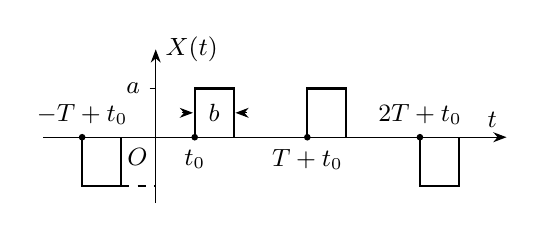
\begin{tikzpicture}[x=0.55cm,y=0.62cm,every node/.style={font=\small},>=Stealth]
  % 坐标轴
  \draw[->] (-2.60,0) -- (8.10,0);
  \node[above left] at (8.10,0) {$t$};
  \draw[->] (0,-1.35) -- (0,1.80);
  \node[right] at (0,1.80) {$X(t)$};
  % 幅度 a 的刻度
  \draw (-0.14,1.00) -- (0,1.00);
  \node[left] at (-0.14,1.00) {$a$};
  % 四个脉冲（宽度 b、幅度 ±a）
  \draw[thick] (-1.70,0) -- (-1.70,-1.00) -- (-0.80,-1.00) -- (-0.80,0);
  \draw[thick] (0.90,0) -- (0.90,1.00) -- (1.80,1.00) -- (1.80,0);
  \draw[thick] (3.50,0) -- (3.50,1.00) -- (4.40,1.00) -- (4.40,0);
  \draw[thick] (6.10,0) -- (6.10,-1.00) -- (7.00,-1.00) -- (7.00,0);
  % 各脉冲起点（时间轴上的圆点）
  \foreach \x in {-1.70,0.90,3.50,6.10}{\fill (\x,0) circle (1.2pt);}
  % -a 的水平虚线（引到纵轴）
  \draw[dashed] (-0.80,-1.00) -- (0,-1.00);
  % 宽度 b 的标注（两个向内箭头 + b）
  \draw[->] (0.60,0.50) -- (0.86,0.50);
  \draw[->] (2.10,0.50) -- (1.84,0.50);
  \node at (1.35,0.50) {$b$};
  % 时间标注
  \node[above] at (-1.70,0.06) {$-T+t_0$};
  \node[anchor=center] at (-0.42,-0.40) {$O$};
  \node[below] at (0.90,-0.06) {$t_0$};
  \node[below] at (3.50,-0.06) {$T+t_0$};
  \node[above] at (6.10,0.06) {$2T+t_0$};
\end{tikzpicture}

\smallskip
{\small 图题3.33}
\end{minipage}\hfill
\begin{minipage}[t]{0.47\linewidth}\centering
% 图题3.34：锯齿波脉冲串；每一周期在 t0+kT 处落到零值，纵轴左侧用虚线画出
% 上一周期的上升段（在 t0-T 处过零）
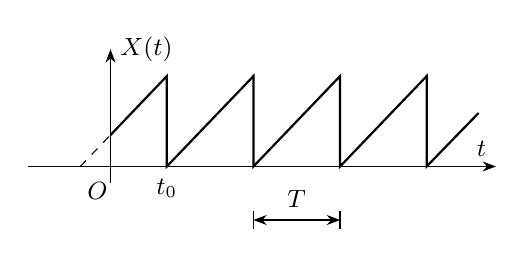
\begin{tikzpicture}[x=0.55cm,y=0.85cm,every node/.style={font=\small},>=Stealth]
  % 坐标轴
  \draw[->] (-1.90,0) -- (8.90,0);
  \node[above left] at (8.90,0) {$t$};
  \draw[->] (0,-0.25) -- (0,1.75);
  \node[right] at (0,1.75) {$X(t)$};
  % 上一周期的上升段（t0-T 处过零，画到纵轴为止，用虚线）
  \draw[dashed] (-0.70,0) -- (0,0.47);
  % 锯齿波：自纵轴起，依次在 t0、t0+T、t0+2T、t0+3T 落到零
  \draw[thick] (0,0.47) -- (1.30,1.35) -- (1.30,0) -- (3.30,1.35) -- (3.30,0)
               -- (5.30,1.35) -- (5.30,0) -- (7.30,1.35) -- (7.30,0) -- (8.50,0.80);
  % 周期 T 的标注（两个相邻的零值时刻之间）
  \draw[<->] (3.30,-0.80) -- (5.30,-0.80);
  \draw (3.30,-0.66) -- (3.30,-0.94);
  \draw (5.30,-0.66) -- (5.30,-0.94);
  \node[above] at (4.30,-0.76) {$T$};
  % 时间标注
  \node[anchor=north] at (-0.30,-0.10) {$O$};
  \node[below] at (1.30,-0.04) {$t_0$};
\end{tikzpicture}

\smallskip
{\small 图题3.34}
\end{minipage}
\end{center}

% EQNUMBERS: （无）
% FIGNUMBERS: 图题3.33, 图题3.34（独立编号，不占 figure 计数器）
% PAGES: 87-88
% EXERCISES: 3.21（仅 (4)(5)(6)） 3.22 3.23 3.24 3.25 3.26 3.27 3.28 3.29 3.30
%            3.31 3.32 3.33 3.34（3.22–3.34 连续无跳号；末题 3.34 后即为书 p.88 页码）

\end{document}
